%!TEX root = ../report.tex
\documentclass[report.tex]{subfiles}
\begin{document}
    \chapter{Evaluation and Results}

    \section{Experiment Description}

    % Describe the experiments/evaluation you are performing to analyse your method.
    \paragraph*{Objective}

    % The primary objective of these experiments is to evaluate the efficacy of three multimodal sensor fusion deep neural network models on two diverse public datasets for object detection in a range of adverse weather conditions. This study aims to understand how tightly-coupled, data-driven multimodal sensor fusion can enhance object detection capabilities in environments where traditional methods may falter due to poor visibility and unpredictable weather elements.

    % This study aims to understand how tightly-coupled, data-driven multimodal sensor fusion can enhance object detection capabilities in environments where traditional methods may falter due to poor visibility and unpredictable weather elements.

    % This study aims to 
    % - Understand how tightly-coupled multimodal sensor fusion can enhance object detection capabilities in environments where conventional methods may falter due to poor visibility and unpredictable weather elements.
    % - Highlight the importance of complementary sensors suit for robust object detection in adverse weather conditions.

    % The primary objective of these experiments is to critically evaluate the efficacy of three multimodal sensor fusion deep neural network models on two diverse public datasets, specifically designed for object detection under a range of adverse weather conditions. This study is conducted with a dual aim. Firstly, it seeks to understand how tightly-coupled multimodal sensor fusion can significantly enhance object detection capabilities, particularly in environments where conventional methods may falter. This faltering is often due to poor visibility and the unpredictability of weather elements, which pose substantial challenges to standard detection techniques. Secondly, the study highlights the importance of employing a complementary suite of sensors. This approach is crucial for ensuring robust object detection in adverse weather conditions, suggesting that the integration of diverse sensor modalities can offer a more comprehensive and reliable solution in challenging environmental contexts.

    The primary objective of these experiments is to critically evaluate the efficacy of three multimodal sensor fusion deep neural network models on two diverse public datasets, specifically designed for object detection under a range of adverse weather conditions. Conducted with a dual aim, this study focuses on:

    \begin{itemize}
        \item \textbf{Understanding Tightly-Coupled Multimodal Sensor Fusion}: Investigating how the integration of multiple sensor types can significantly enhance object detection capabilities in environments where traditional methods are less effective. This is particularly relevant in scenarios with poor visibility and unpredictable weather elements, where standard detection techniques may struggle.
        \item \textbf{Highlighting the Importance of Complementary Sensors}: Emphasizing the necessity of employing a suite of complementary sensors for robust object detection in challenging weather conditions. This approach underlines the value of diverse sensor modalities working in concert to provide a more reliable and comprehensive solution for object detection in adverse environmental contexts.
    \end{itemize}

    \paragraph*{Relevance to Adverse Weather Conditions}

    This research tackles the significant challenges posed by adverse weather conditions such as heavy rain, fog, and snow, which greatly affect the accuracy of object detection systems essential in autonomous navigation and outdoor surveillance. Acknowledging the limitations of commonly used sensors like cameras and LiDAR in inclement weather, contrasted with the robustness of Radar, the study emphasizes integrating multimodal sensor data to bolster the robustness and reliability of object detection in these environments. This study provides a comprehensive overview and detailed analysis of existing top methods, elucidating their efficacy and limitations in diverse weather scenarios, thereby informing best practices in the field.

    \paragraph*{Experiment Overview}

    % TODO: if it is verbose, then shorten it
    \begin{itemize}
        \item \textbf{Objective of the Experiments:} The main aim of these experiments is to explore the strengths and weaknesses of using camera-only systems compared to systems that incorporate multiple sensor modalities, especially in challenging weather conditions.

        \item \textbf{Comparative Analysis of Fusion Architectures:} A key focus of the experiments is to compare the performance of tightly-coupled fusion architectures with conventional fusion architectures. This comparison is intended to provide insights into how different fusion methodologies impact the accuracy and reliability of object detection in adverse weather conditions.

        \item \textbf{Datasets Used for Evaluation:} The experiments utilize two major public datasets, namely nuScenes and DENSE, to provide a broad and comprehensive evaluation of the models. These datasets are particularly relevant as they include a variety of adverse weather conditions that pose challenges to object detection systems.

        \item \textbf{Performance Metrics and Evaluation:} The results of the experiments are quantified and presented using COCO style metrics. This choice of metric allows for a standardized comparison of model performance.

        \item \textbf{Weather-Specific Analysis:} Where possible, results are presented in the context of specific weather conditions. This approach helps to highlight how each model performs under various types of adverse weather, providing a more nuanced understanding of their capabilities and limitations.

        \item \textbf{Experiment Setup and Methodology:} Detailed descriptions of the experimental setup, including the specifics of the sensor arrays used, the configuration of the neural network models, and the criteria for evaluating their performance.

        \item \textbf{Interpretation of Results:} A thorough analysis of the experimental results, focusing on the efficacy of multimodal sensor fusion in improving object detection in adverse weather, and discussing the implications of these findings for the field of autonomous vehicles.
    \end{itemize}

    \section{Experimental Setup}

        \subsection{Hardware and Software Configuration}
        \begin{itemize}
            \item \textbf{Sensor Array Configuration:} The experiments utilized two multimodal datasets, which primarily comprise the following sensors:
                \begin{itemize}
                    \item RGB camera
                    \item LiDAR
                    \item Radar
                \end{itemize}
                These sensors were selected due to their varied capabilities in capturing environmental data under different weather conditions, as detailed in the respective dataset descriptions.

            \item \textbf{Computational Resources:} The experiments were conducted using HBRS University's High Performance Scientific Computing (HPC) \cite{hbrs_scientificComputing2023}, equipped multiple GPU devices, such as:
                \begin{itemize}
                    \item NVIDIA V100 GPU with 16GB memory
                    \item NVIDIA A100 GPU with 80GB memory
                \end{itemize}
                Additionally, for debugging purposes, lab computing resources featuring an NVIDIA RTX 3090 GPU with 24GB memory were utilized. For more details, please refer to the appendix \ref{appendix:gpu_details}. 

            \item \textbf{Software Environment:} The experiments employed the PyTorch framework for training and evaluation of the three methods. Specifically, two methods were implemented using the MMDetection framework, built on top of PyTorch, to facilitate the development of object detection models. Below Table \ref{tab:pytorch_versions} shows the PyTorch versions used for each method.
            
            \begin{table}[h]
                \centering
                \caption{PyTorch and CUDA versions}
                \begin{tabular}{|l|l|l|}
                \hline
                \textbf{Methods} & \textbf{PyTorch} & \textbf{CUDA} \\ \hline
                SAF-FCOS & 1.12 & 11.6 \\ \hline
                HRFuser & 1.10 & 10.2 / 11.1 \\ \hline
                MT-DETR & 1.10 & 11.1 \\ \hline
                \end{tabular}
                \label{tab:pytorch_versions}
            \end{table}
        \end{itemize}

        \subsection{Datasets}
        \begin{itemize}
            \item \textbf{Dataset Description:} A detailed description of the datasets used in the experiments is provided in Section~\ref{sec:available_datasets}. It is important to note that, although both datasets offer 360-degree perception coverage, the methods employed in this study utilized only the front-view sensors for training.

            \item \textbf{Data Preprocessing:} In addition to the projection methods outlined in Section~\ref{sec:selected_methods}, the experiments incorporated basic data augmentation techniques: RandomFlip, RandomCrop, and RandomDrop. Note that `RandomDrop' is an augmentation method where sensor streams in multimodal architectures are randomly omitted with a specified probability. The table below outlines the specific augmentation techniques employed for each method in the experiments:
                \begin{table}[h]
                    \centering
                    \caption{Methods and augmentation techniques}
                    \begin{tabular}{|l|l|}
                    \hline
                    \textbf{Methods} & \textbf{Augmentation Techniques} \\ \hline
                    SAF-FCOS & RandomFlip, Crop, Resize \\ \hline
                    HRFuser & RandomFlip, Crop, Resize, RandomDrop \\ \hline
                    MT-DETR & RandomFlip, RandomCrop, Resize \\ \hline
                    \end{tabular}
                    \label{tab:methods_augmentation}
                \end{table}

            \item \textbf{Dataset Split:} 
            
            \paragraph*{SAF-FCOS}

            The method limits its focus on detecting vehicular obstacles such as — bicycles, cars, motorcycles, buses, trailer, and trucks—collectively categorized as 'vehicles' for simplified classification. Pedestrians are excluded due to Radar detection limitations in the nuScenes dataset. Emphasis is placed on front camera data from nuScenes, with the dataset split detailed in Figure \ref{fig:saffcos_data_split}.

            \begin{figure}[h!]
                \centering
                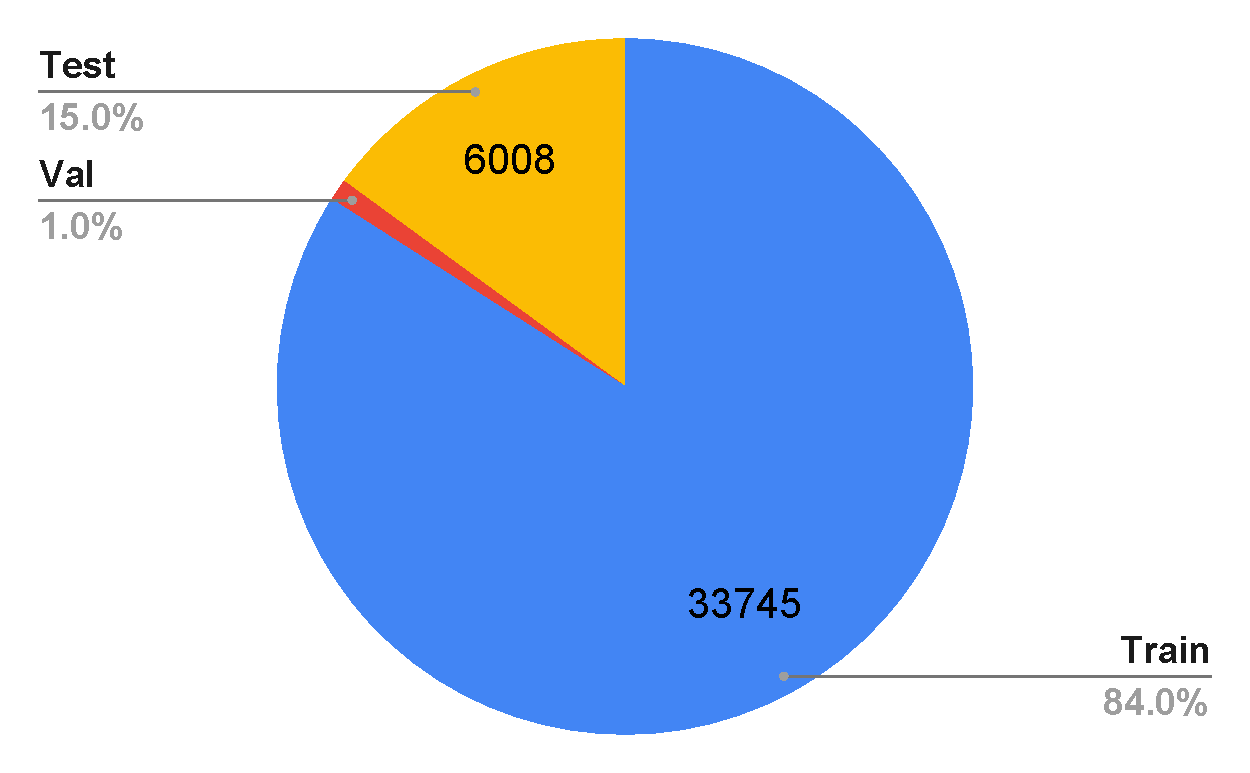
\includegraphics[width=0.6\textwidth]{images/methods/saf_fcos/data_split.pdf}
                \caption{Data split of nuScenes dataset. Total samples: 40157. Note: this is a custom dataset split chosen by the authors.}
                \label{fig:saffcos_data_split}
            \end{figure}

            \paragraph*{HRFuser}

            The original HRFuser approach employs ten superclasses derived from the nuScenes dataset for its training and evaluation protocols. Table \ref{tab:hrfuser_classes_nuscenes} delineates the correspondence between nuScenes and HRFuser class categorizations. To facilitate a direct comparison with SAF-FCOS, we adopted identical class designations and data partitions as delineated in SAF-FCOS. This alignment extends to the annotation process. As detailed in Section \ref{subsec:nuscenes_dataset}, the nuScenes dataset omits 2D annotations for its test set. Consequently, the SAF-FCOS framework generated proprietary annotations for this subset by leveraging an augmented version of FCOS supplemented with manual adjustments. To synchronize our performance metrics, we have created a custom annotation conversion script that reformats SAF-FCOS annotations into the HRFuser schema. This utility underscores the variance in annotation formats within multimodal datasets, despite both methodologies utilizing COCO-style annotations. The conversion script is accessible in our code repository for replication and further research endeavors.

            \begin{table}[h]
                \centering
                \caption{Mapping from nuScenes classes to HRFuser classes \cite{caesar2020nuscenes}}
                \begin{tabular}{|l|l|}
                \hline
                \textbf{NuScenes Class} & \textbf{Mapped Class} \\ \hline
                vehicle.car & car \\ \hline
                vehicle.truck & truck \\ \hline
                vehicle.trailer & trailer \\ \hline
                vehicle.bus.bendy & bus \\ \hline
                vehicle.bus.rigid & bus \\ \hline
                vehicle.construction & construction\_vehicle \\ \hline
                vehicle.bicycle & bicycle \\ \hline
                vehicle.motorcycle & motorcycle \\ \hline
                human.pedestrian.child & pedestrian \\ \hline
                human.pedestrian.adult & pedestrian \\ \hline
                human.pedestrian.construction\_worker & pedestrian \\ \hline
                human.pedestrian.police\_officer & pedestrian \\ \hline
                movable\_object.trafficcone & traffic\_cone \\ \hline
                movable\_object.barrier & barrier \\ \hline
                \end{tabular}
                \label{tab:hrfuser_classes_nuscenes}
            \end{table}
                

            For DENSE dataset, the method uses 3 classes for training and evaluation, namely Car, Pedestrian, and Cyclist, Table \ref{tab:hrfuser_classes_dense} shows the mapping from DENSE classes to HRFuser classes. The dataset split is shown in Figure \ref{fig:hrfuser_data_split_dense}.

            \begin{table}[h]
                \centering
                \caption{Mapping from DENSE classes to HRFuser classes \cite{broedermann2022hrfuser}}
                \begin{tabular}{|l|l|}
                \hline
                \textbf{DENSE Class} & \textbf{Mapped Class} \\ \hline
                PassengerCar         & Car                   \\ \hline
                Pedestrian           & Pedestrian            \\ \hline
                RidableVehicle       & Cyclist               \\ \hline
                Large Vehicle        & Car                   \\ \hline
                DontCare             & DontCare              \\ \hline
                \end{tabular}
                
                \label{tab:hrfuser_classes_dense}
            \end{table}

            \begin{figure}[h!]
                \centering
                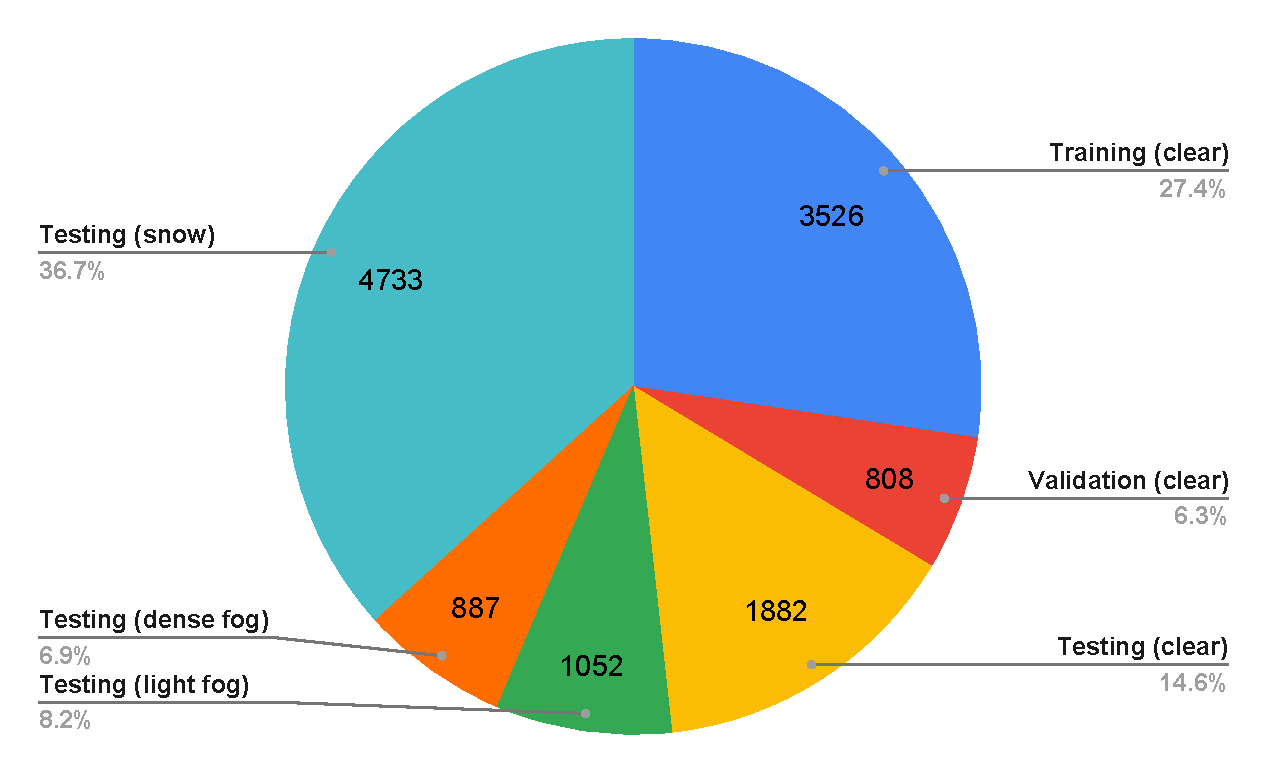
\includegraphics[width=0.7\textwidth]{images/datasets/dense/dataset_split.pdf}
                \caption{Data split for DENSE dataset. Total samples: 12888. Note: all methods use clear weather data for training and validation, and use adverse weather data for testing.}
                \label{fig:hrfuser_data_split_dense}
            \end{figure}

            \paragraph*{MT-DETR}

            The MT-DETR model adopts a distinct class categorization for training and evaluation purposes, on the DENSE dataset. Specifically, it combines the 'Car' and 'Cyclist' classes into a unified 'Vehicle' category while maintaining 'Pedestrian' as a standalone class. Consequently, the MT-DETR conducts its training and evaluation processes on these two distinct classes. It is important to note that MT-DETR follows the same dataset partitioning as utilized in the HRFuser framework, which is delineated in Figure \ref{fig:hrfuser_data_split_dense}.

            It is important to emphasize that the methods employing the DENSE dataset are trained exclusively on data from clear weather conditions. However, their testing is conducted on a set that encompasses a variety of extremely challenging weather scenarios. This approach serves to assess the methods' robustness, particularly in situations where one sensor may fail due to adverse conditions. The focus is on how effectively these methods utilize the remaining operational sensors to maintain accurate object detection. Such testing is crucial in understanding the resilience and adaptability of the methods under diverse and unpredictable environmental circumstances.

                
        \end{itemize}

        \subsection{Model Configuration and Training}
        \begin{itemize}
            
            \item \textbf{Training Parameters:} The Table \ref{tab:experiment_training_parameters} below represents typical training configurations for each method employed in this project. However, the original settings varied from these due to GPU computational constraints. In addition, all methods implement learning rate decay and warmup schemes. It should be noted that the asterisk (*) in the table denotes the total batch size when the model is trained across multiple GPUs.
            
            The model checkpoint with the lowest validation loss is used for evaluation on the test set. The training parameters for each method are detailed below:

            \begin{table}[h]
                \centering
                \caption{Training parameters. (*) denotes total batch size for models trained on multiple GPUs.}
                \begin{tabular}{|l|l|l|l|l|l|}
                \hline
                \textbf{Methods} & \textbf{Optimizer} & \textbf{Learn. Rate} & \textbf{Batch Size} & \textbf{Epochs} & \textbf{Input (WxH)} \\ \hline
                SAF-FCOS         & SGD                & 0.001                & 8                   & 12              & 1333 x 800           \\ \hline
                HRFuser (nuScenes) & AdamW             & 0.0003               & 12*                 & 12              & 640x384              \\ \hline
                HRFuser (DENSE)    & AdamW             & 0.001                & 12*                 & 60              & 1284x384             \\ \hline
                MT-DETR            & AdamW             & 0.0001               & 1                   & 36              & 1333 x 800           \\ \hline
                \end{tabular}
                \label{tab:experiment_training_parameters}
            \end{table}
            
            
            \item \textbf{Evaluation Metrics:} For the evaluation of the models, the COCO style evaluation metrics were adopted. For each method and its respective configuration, we provide comprehensive details including the total number of model parameters, floating point operations, and the inference time. The details are described in Section~\ref{sec:metrics}.
            
            For every method and in all experimental combinations, the model inference confidence threshold is set to 0.3, in accordance with the threshold specified in the original paper.
        \end{itemize}

        

        
        \subsection{Experimental Procedure}
        \begin{itemize}
            \item \textbf{Testing Protocol:} To facilitate a comprehensive quantitative analysis, all models were evaluated using test sets from both datasets. For comparative purposes, Average Precision (AP) and Average Recall (AR) metrics were employed. Additionally, the models were assessed in terms of complexity, considering aspects such as the number of model parameters, floating-point operations, and inference time. Here, the inference time (or FPS) is calculated based on the average time it takes to process a single image on the test set. For floating-point operations, it is calculated with batch size 1. For qualitative analysis, images showcasing model predictions alongside ground truth on the test sets were provided for most relevant experiments. In the following experiments, loss curves have not been included. This is because each method employs a distinct loss calculation approach, rendering direct comparisons between them impractical.
            \item \textbf{All Experiments Combinations:} The table referenced as Table \ref{tab:total_available_configurations} presents all the available configurations for each method. And table below that Table \ref{tab:experiment_combinations}, listed an overview of all the experiments done for this project. Note that only the experiment listed with Sr. 1 is conducted on the nuScenes dataset; the rest are all on the DENSE dataset.

            \begin{table}[h!]
                \centering
                \caption{Available configurations for each method.}
                \begin{tabular}{|l|c|c|c|c|c|c|c|}
                \hline
                \textbf{Methods} & \textbf{Early} & \textbf{Middle} & \textbf{Tightly-coupled} & \textbf{Camera} & \textbf{LiDAR} & \textbf{Radar} & \textbf{Extra} \\ \hline
                SAF-FCOS & $\times$ & $\checkmark$ & $\times$ & $\checkmark$ & $\times$ & $\checkmark$ & $\times$ \\ \hline
                HRFuser & $\times$ & $\times$ & $\checkmark$ & $\checkmark$ & $\checkmark$ & $\checkmark$ & Gated \\ \hline
                MT-DETR & $\checkmark$ & $\checkmark$ & $\checkmark$ & $\checkmark$ & $\checkmark$ & $\checkmark$ & Time \\ \hline
                \end{tabular}
                \label{tab:total_available_configurations}
            \end{table}
            

                \begin{table}[h!]
                    \centering
                    \caption{Overview of experiment combinations. C, L, R, G, and T denote Camera, LiDAR, Radar, Gated camera, and Time}
                    \begin{tabular}{|c|l|l|c|c|c|c|c|c|l|}
                    \hline
                    \textbf{Sr.} & \multicolumn{2}{c|}{\textbf{Method}} & \multicolumn{3}{c|}{\textbf{Fusion Architecture}} & \multicolumn{3}{c|}{\textbf{Sensors}} & \textbf{Extra} \\
                    \cline{2-9}
                     & \textbf{1} & \textbf{2} & \textbf{Early} & \textbf{Middle} & \textbf{Tightly-c.} & \textbf{C} & \textbf{L} & \textbf{R} &  \\
                    \hline
                    1 & SAF-FCOS & HRFuser & $\times$ & $\checkmark$ & $\checkmark$ & $\checkmark$ & $\times$ & $\checkmark$ & $\times$ \\
                    \hline
                    2 & HRFuser & - & $\times$ & $\times$ & $\checkmark$ & $\checkmark$ & $\checkmark$ & $\checkmark$ & $\times$ \\
                    \hline
                    3 & HRFuser & - & $\times$ & $\times$ & $\checkmark$ & $\checkmark$ & $\checkmark$ & $\checkmark$ & G \\
                    \hline
                    4 & MT-DETR & - & $\checkmark$ & $\times$ & $\times$ & $\checkmark$ & $\checkmark$ & $\checkmark$ & $\times$ \\
                    \hline
                    5 & MT-DETR & - & $\times$ & $\checkmark$ & $\times$ & $\checkmark$ & $\checkmark$ & $\checkmark$ & $\times$ \\
                    \hline
                    6 & MT-DETR & - & $\times$ & $\times$ & $\checkmark$ & $\checkmark$ & $\checkmark$ & $\checkmark$ & $\times$ \\
                    \hline
                    7 & MT-DETR & - & $\checkmark$ & $\checkmark$ & $\checkmark$ & $\checkmark$ & $\times$ & $\checkmark$ & $\times$ \\
                    \hline
                    8 & MT-DETR & - & $\checkmark$ & $\checkmark$ & $\checkmark$ & $\checkmark$ & $\checkmark$ & $\checkmark$ & $\times$ \\
                    \hline
                    9 & MT-DETR & - & $\times$ & $\times$ & $\checkmark$ & $\checkmark$ & $\checkmark$ & $\checkmark$ & T \\
                    \hline
                    10 & HRFuser & MT-DETR & $\times$ & $\times$ & $\times$ & $\checkmark$ & $\times$ & $\times$ & $\times$ \\
                    \hline
                    11 & HRFuser & MT-DETR & $\times$ & $\times$ & $\checkmark$ & $\checkmark$ & $\times$ & $\checkmark$ & $\times$ \\
                    \hline
                    12 & HRFuser & MT-DETR & $\times$ & $\times$ & $\checkmark$ & $\checkmark$ & $\checkmark$ & $\times$ & $\times$ \\
                    \hline
                    13 & HRFuser & MT-DETR & $\times$ & $\times$ & $\checkmark$ & $\checkmark$ & $\checkmark$ & $\checkmark$ & $\times$ \\
                    \hline
                    14 & HRFuser & MT-DETR & $\times$ & $\times$ & $\checkmark$ & $\checkmark$ & $\checkmark$ & $\checkmark$ & G,T \\
                    \hline
                    \end{tabular}
                    \label{tab:experiment_combinations}
                \end{table}
                
            \textbf{NOTE: The majority of the experiments were carried out utilizing the DENSE dataset in conjunction with the MT-DETR method. Due to computational complexities and resource constraints, it is not feasible to evaluate every possible combination.}
                
        \end{itemize}
    
    % ####################################################################
    % #####################################################
    % ################################################################

    \section{Results}

    For all the experiments below, C, L, R, G, and T denote Camera, LiDAR, Radar, Gated camera, and Time respectively. For better readability and visibility, legends color code are maintained same for each sensor modality. All plots are best visualized in zoomed-in view.

    To get the complete result table for all the experiments carried out on the DENSE dataset, please refer to Table \ref{tab:complete_results_table}.

    \subsection{SAF-FCOS vs. HRFuser}

    In this section, we conduct an evaluation of the performance of two distinct methods on the nuScenes test dataset. The first method, SAF-FCOS, utilizes a Middle Fusion architecture, while the second method, HRFuser, is built upon a Tightly-Coupled Fusion architecture. It is important to note that this Experiment is focused only on the fusion of Camera and Radar sensor data. The results are presented in accordance with COCO-style metrics, as outlined in Table \ref{tab:coco_metrics}.

    \begin{figure}[h!]
        \centering
        \begin{subfigure}[b]{0.45\textwidth}
            \centering
            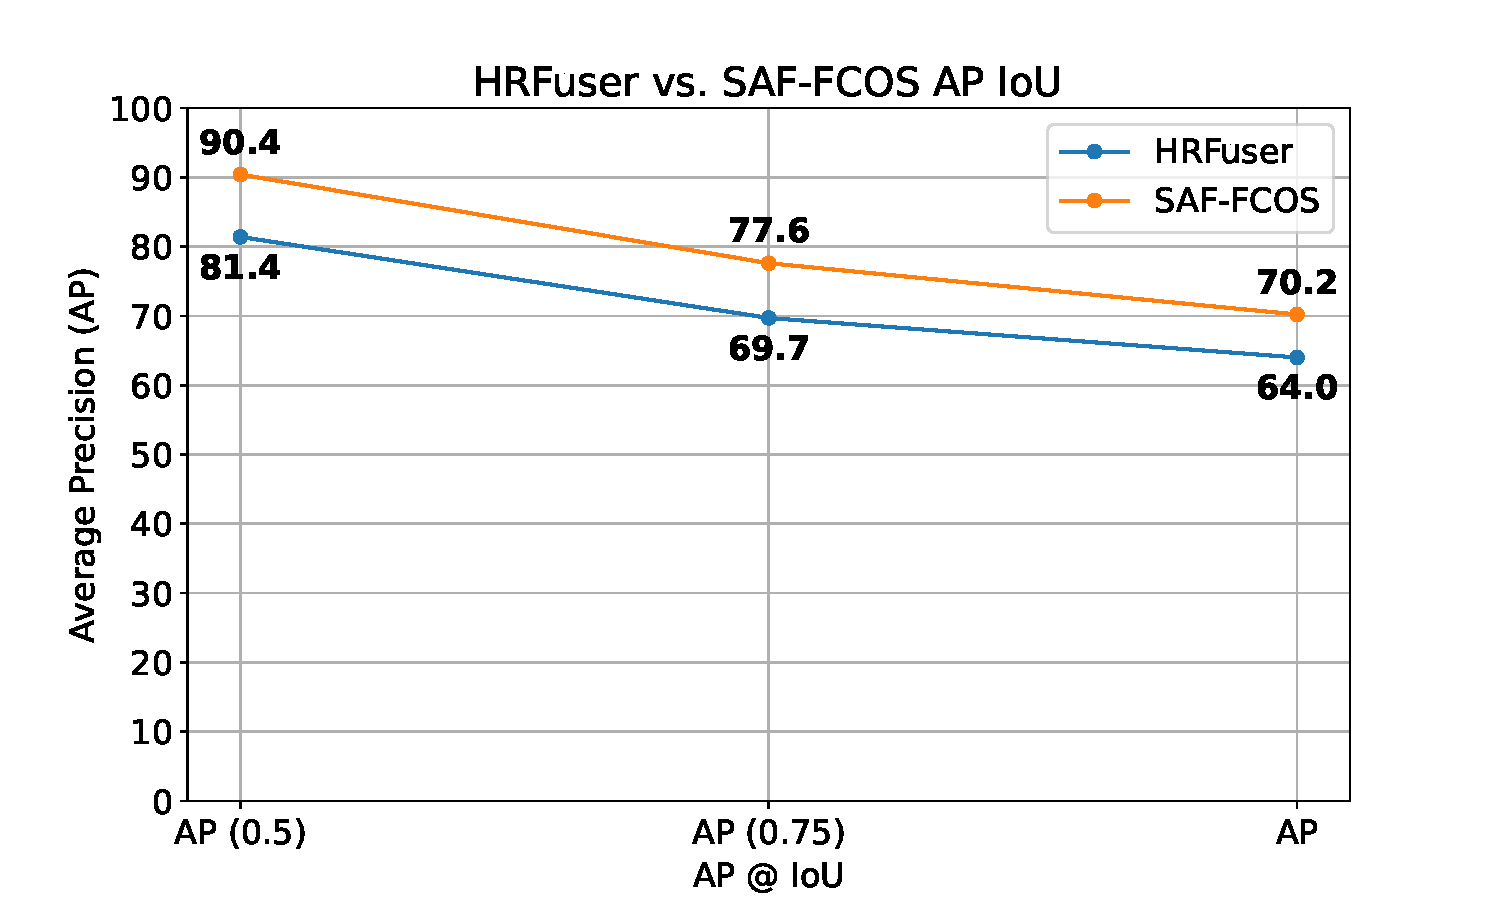
\includegraphics[width=\textwidth]{images/results/saf_vs_hrfuser/ap_iou.pdf}
            \caption{Average Precision (AP)}
            \label{fig:saf_vs_hrfuser_ap_iou}
        \end{subfigure}
        \hfill % adds horizontal space between figures
        \begin{subfigure}[b]{0.45\textwidth}
            \centering
            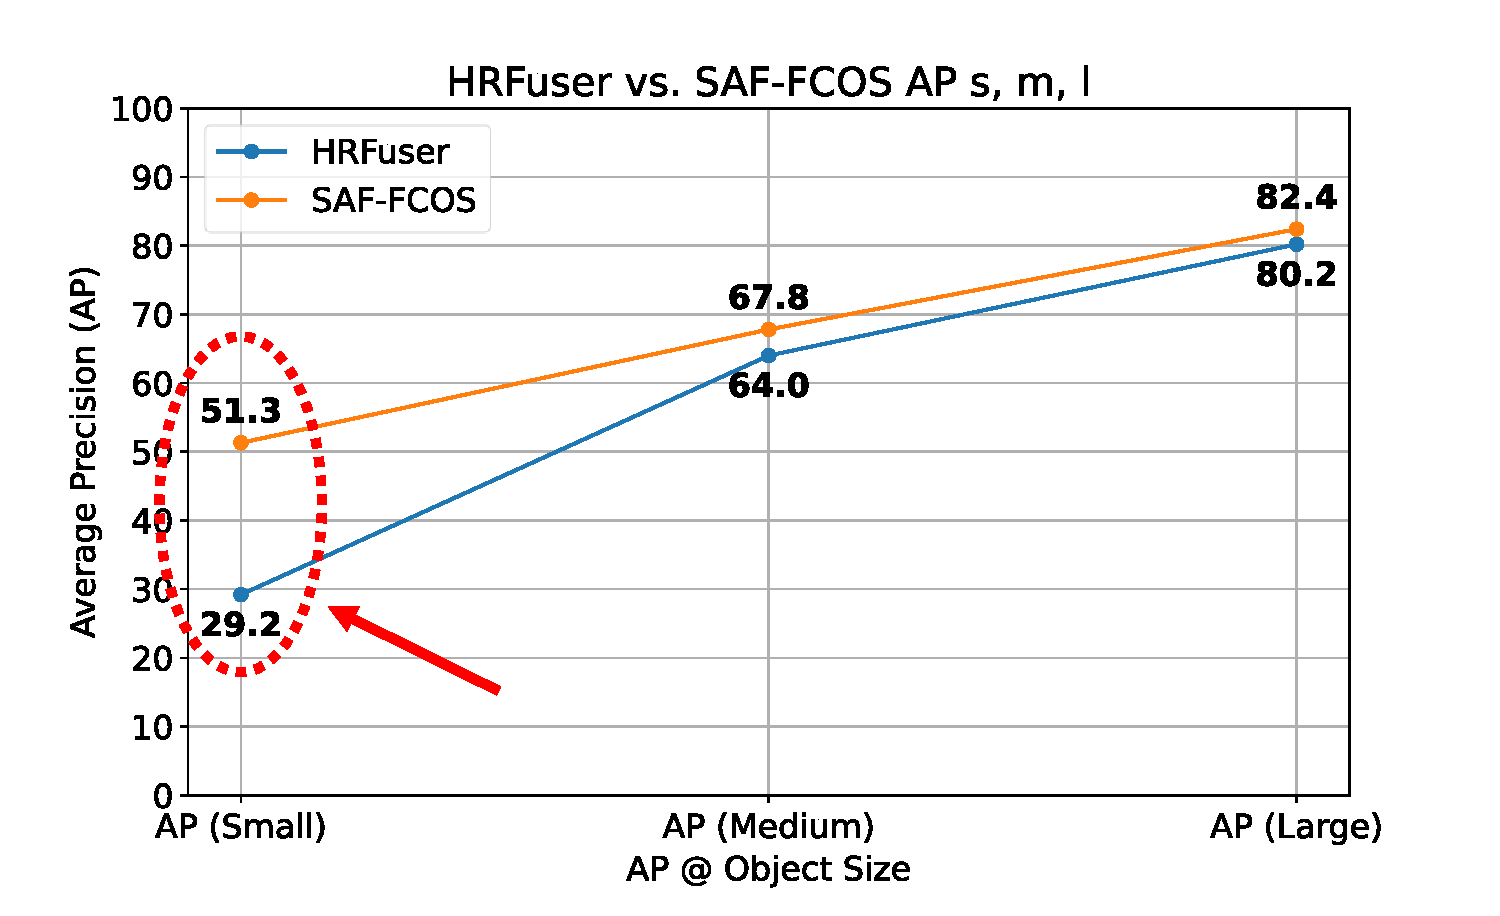
\includegraphics[width=\textwidth]{images/results/saf_vs_hrfuser/ap_sml_anno.pdf}
            \caption{Average Precision (AP) at S, M, L}
            \label{fig:saf_vs_hrfuser_ap_sml}
        \end{subfigure}
        \vspace{1em} % adds vertical space between rows
        \begin{subfigure}[b]{0.45\textwidth}
            \centering
            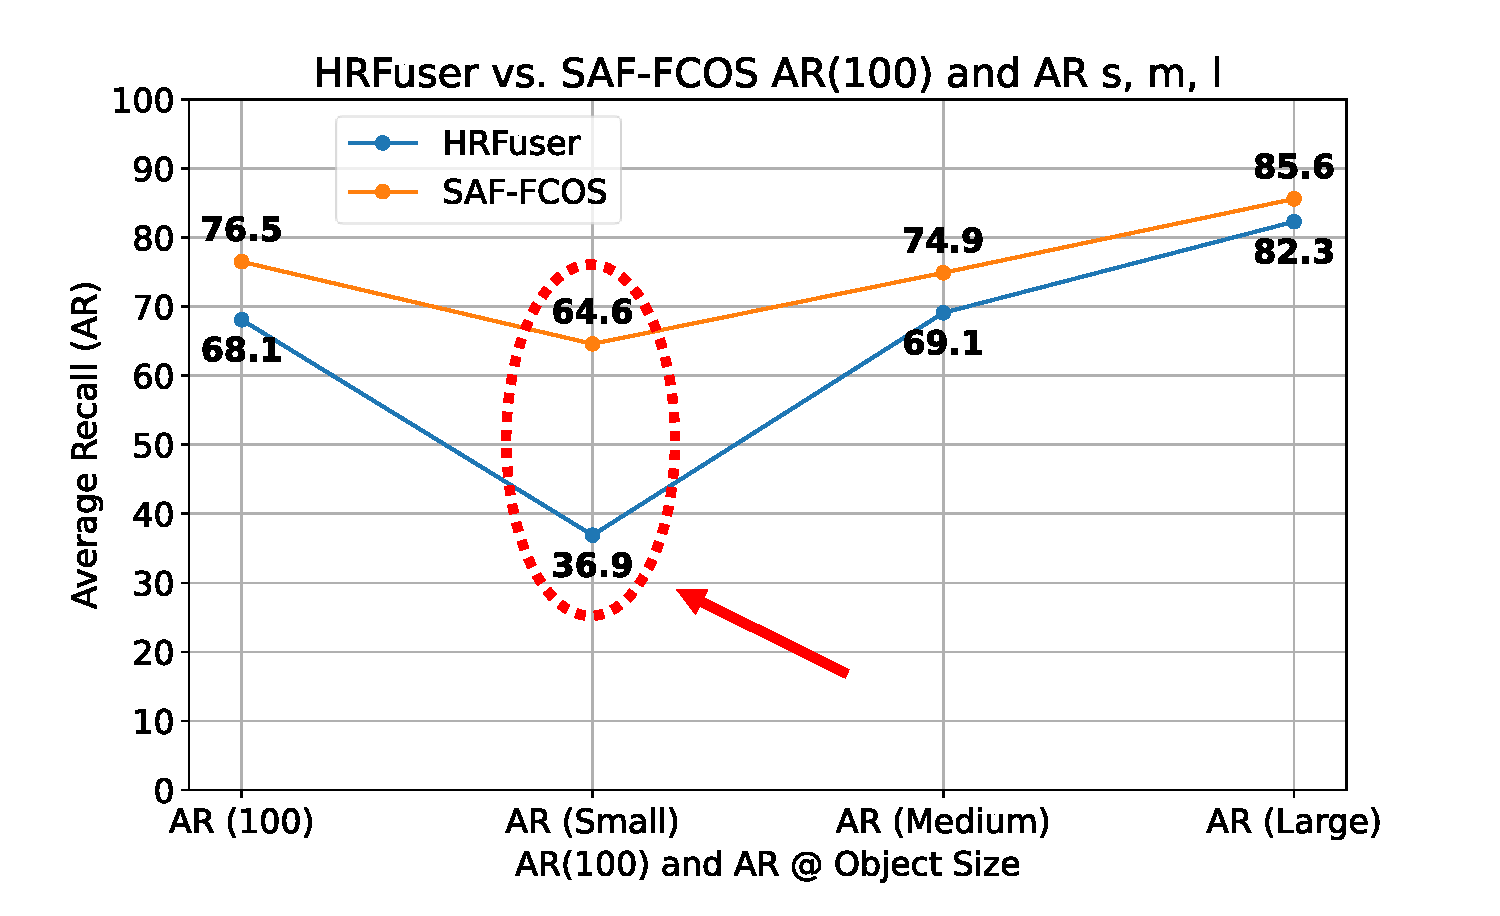
\includegraphics[width=\textwidth]{images/results/saf_vs_hrfuser/ar_anno.pdf}
            \caption{Average Recall (AR)}
            \label{fig:saf_vs_hrfuser_ar}
        \end{subfigure}
        \hfill
        \begin{subfigure}[b]{0.45\textwidth}
            \centering
            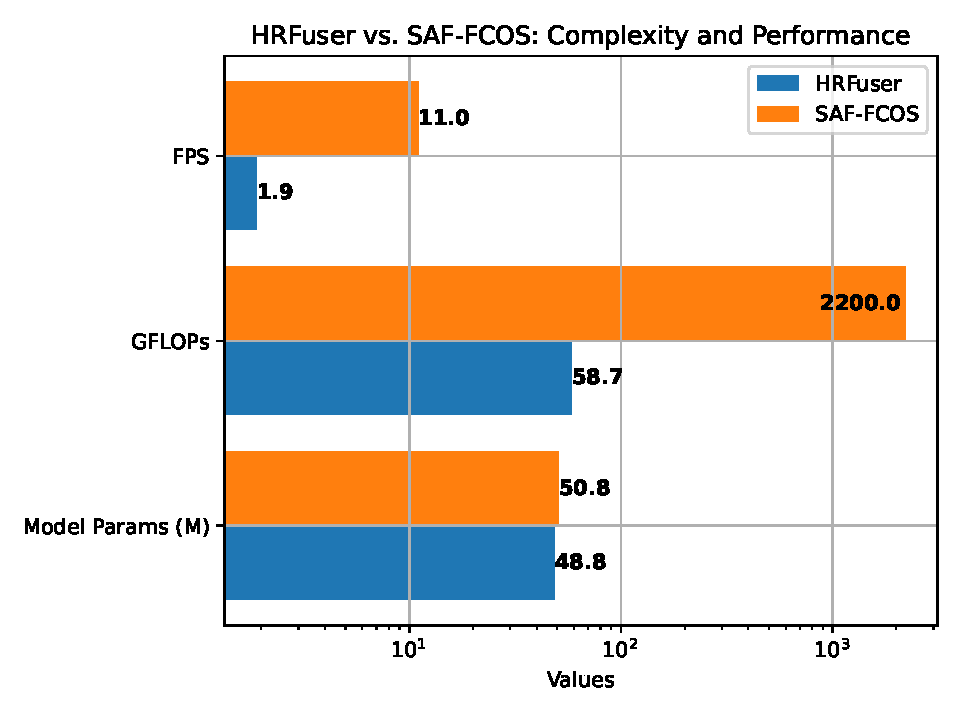
\includegraphics[width=\textwidth]{images/results/saf_vs_hrfuser/model_complexity.pdf}
            \caption{Model Complexity}
            \label{fig:saf_vs_hrfuser_model_complexity}
        \end{subfigure}
        \caption{Comparative Analysis: (a) Comparison on Average Precision (AP) at different IoU thresholds. Note AP@0.5:0.05:0.95 is the mean AP across all IoU thresholds. (b) Comparison on Average Precision (AP) at different object sizes. (c) Comparison on Average Recall (AR) with AR(100) and at different object sizes. (d) Comparison in terms of model parameters (M), computational complexity (GFLOPs), and frame rate (FPS).}
        \label{fig:comparative_analysis}
    \end{figure}

    % From the quantitative comparison, it can be clearly concluded that SAF-FCOS outperforms HRFuser in all metrics. It is important to note here that despite having slightly more model parameters (+2 M) than HRFuser, the FPS value is significantly higher, 11 vs. 1.9 FPS. The possible reason could be due to the fact that SAF-FCOS uses single-stage detector while HRFuser uses two-stage detector. However, surprisingly, from the model complexity Fig. \ref{fig:saf_vs_hrfuser_model_complexity} (d), it seems that SAF-FCOS having a huge x36 times more floating-point operations than its counterpart HRFuser. One possible reason behind this is that floating-point operations are highly dependent on the input size of the sample. In this comparison, as described in the Table \ref{tab:experiment_training_parameters}, SAF-FCOS is using much larger input than the HRFuser. So for this reason, the GFLOPs value is much higher than HRFuser. Also from the annotated figures \ref{fig:comparative_analysis} (b) and (c), it is observable that the performance gap between SAF-FCOS and HRFuser is much larger for small objects. This points to the advantage of using Spatial Attention Fusion (SAF) block in the SAF-FCOS architecture, which was specifically added to gain as much as information possible from the sparse Radar data. So overall, for this particular experiment, it seems that Middle Fusion architecture is more robust than Tightly-Coupled Fusion architecture on nuScenes test dataset.


    The comparative analysis demonstrates a clear superiority of SAF-FCOS over HRFuser across all metrics. Notably, SAF-FCOS exhibits a remarkable frame rate of 11 FPS, significantly outstripping HRFuser's 1.9 FPS, despite having a marginally higher model parameter count (+2M). This performance disparity is likely attributable to SAF-FCOS's utilization of a single-stage detector, as opposed to HRFuser's two-stage approach. Contrasting this, an examination of model complexity, as illustrated in Fig. \ref{fig:saf_vs_hrfuser_model_complexity} (d), reveals an unexpected finding: SAF-FCOS requires substantially more floating-point operations — a factor of 36 times greater than HRFuser. A plausible explanation for this discrepancy is the dependency of floating-point operations on input size. As indicated in Table \ref{tab:experiment_training_parameters}, SAF-FCOS processes considerably larger inputs compared to HRFuser, resulting in a heightened GFLOPs value.

    Further scrutiny, particularly of the annotated figures \ref{fig:comparative_analysis} (b) and (c), discloses a more pronounced performance differential in the detection of smaller objects. This observation underscores the efficacy of the Spatial Attention Fusion (SAF) block integrated within the SAF-FCOS framework. The SAF block's inclusion is a strategic enhancement aimed at maximizing the extraction of information from sparse Radar data. Consequently, in this specific experimental context using the nuScenes test dataset, the Middle Fusion architecture, exemplified by SAF-FCOS, demonstrates a robustness surpassing that of the Tightly-Coupled Fusion architecture, as represented by HRFuser.

    \paragraph*{Qualitative Analysis}

    The effectiveness of SAF-FCOS and HRFuser methods in different weather conditions is clearly demonstrated in the nuScenes test set. Figure \ref{fig:saf_vs_hrfuser} shows various scenarios. The first row shows how these methods detect objects in bright daylight, where many objects are present. The second row focuses on night conditions, where it's harder to see objects due to low light. The third row shows detection during rain, with the camera lens affected by water, yet both models still successfully identify objects. Importantly, rows four and five compare the detection of small, distant objects. Here, SAF-FCOS proves to be more effective than HRFuser, highlighting its better performance in spotting smaller objects that are far away. This performance underscores the significance of the long detection range of Radar sensors, with SAF-FCOS effectively extracting relevant information from these challenging scenarios. This comparison is crucial for understanding how each method performs under different conditions.

    \begin{figure}[h!]
        \centering
        % Row 1
        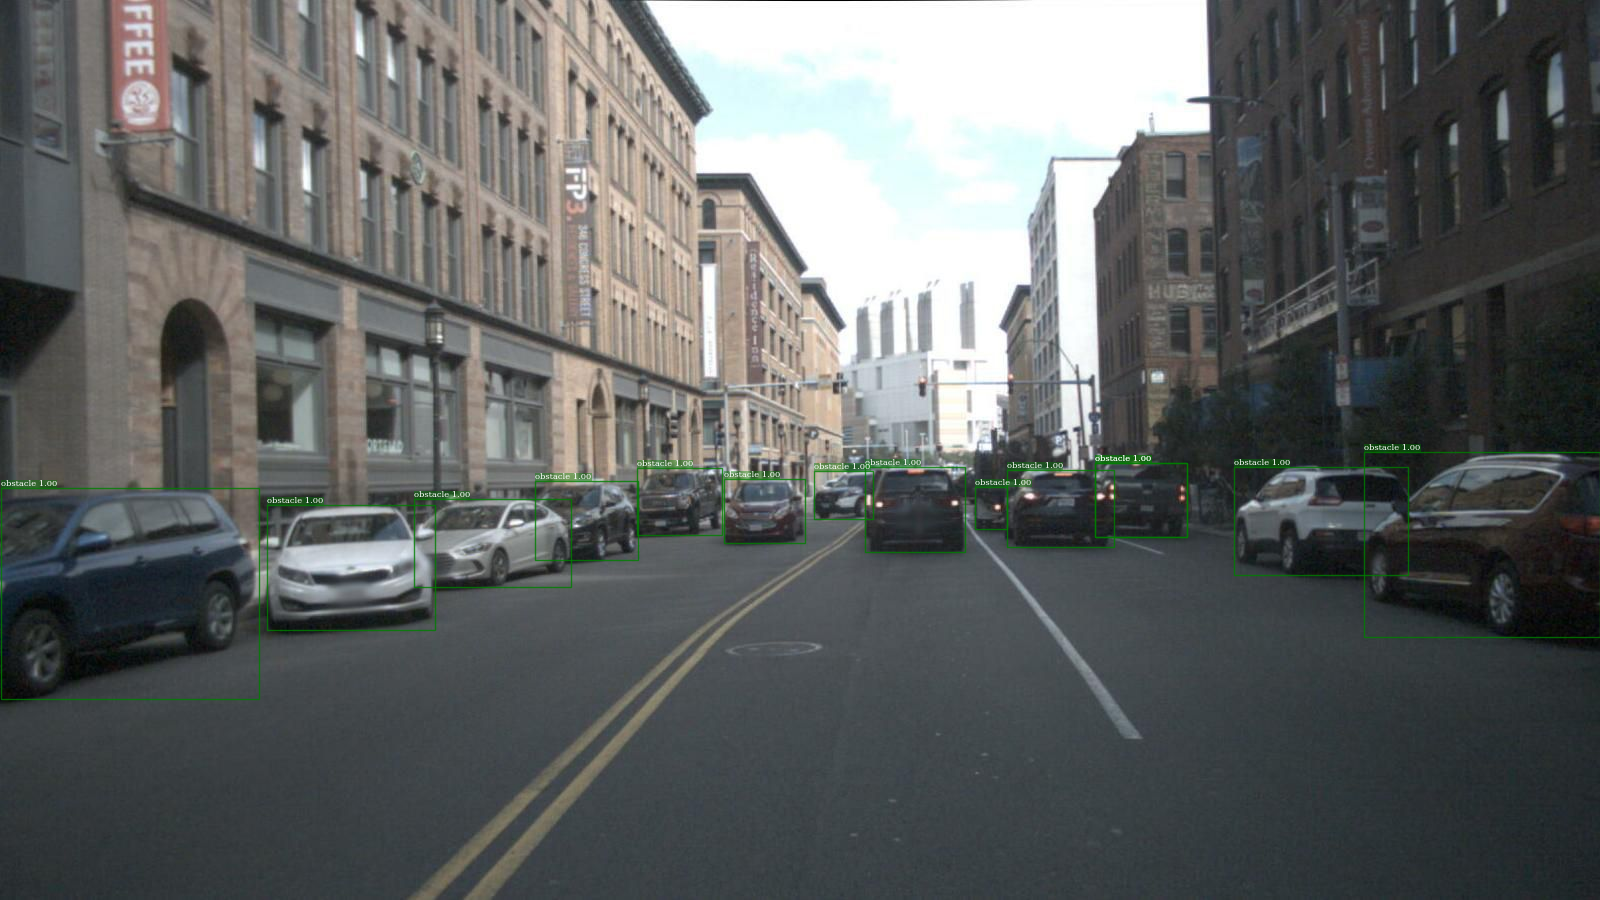
\includegraphics[width=0.3\textwidth]{images/results/saf_vs_hrfuser/samples/s3_day_regular/n008-2018-08-01-15-34-25-0400__CAM_FRONT__1533152655412404_gt.png}
        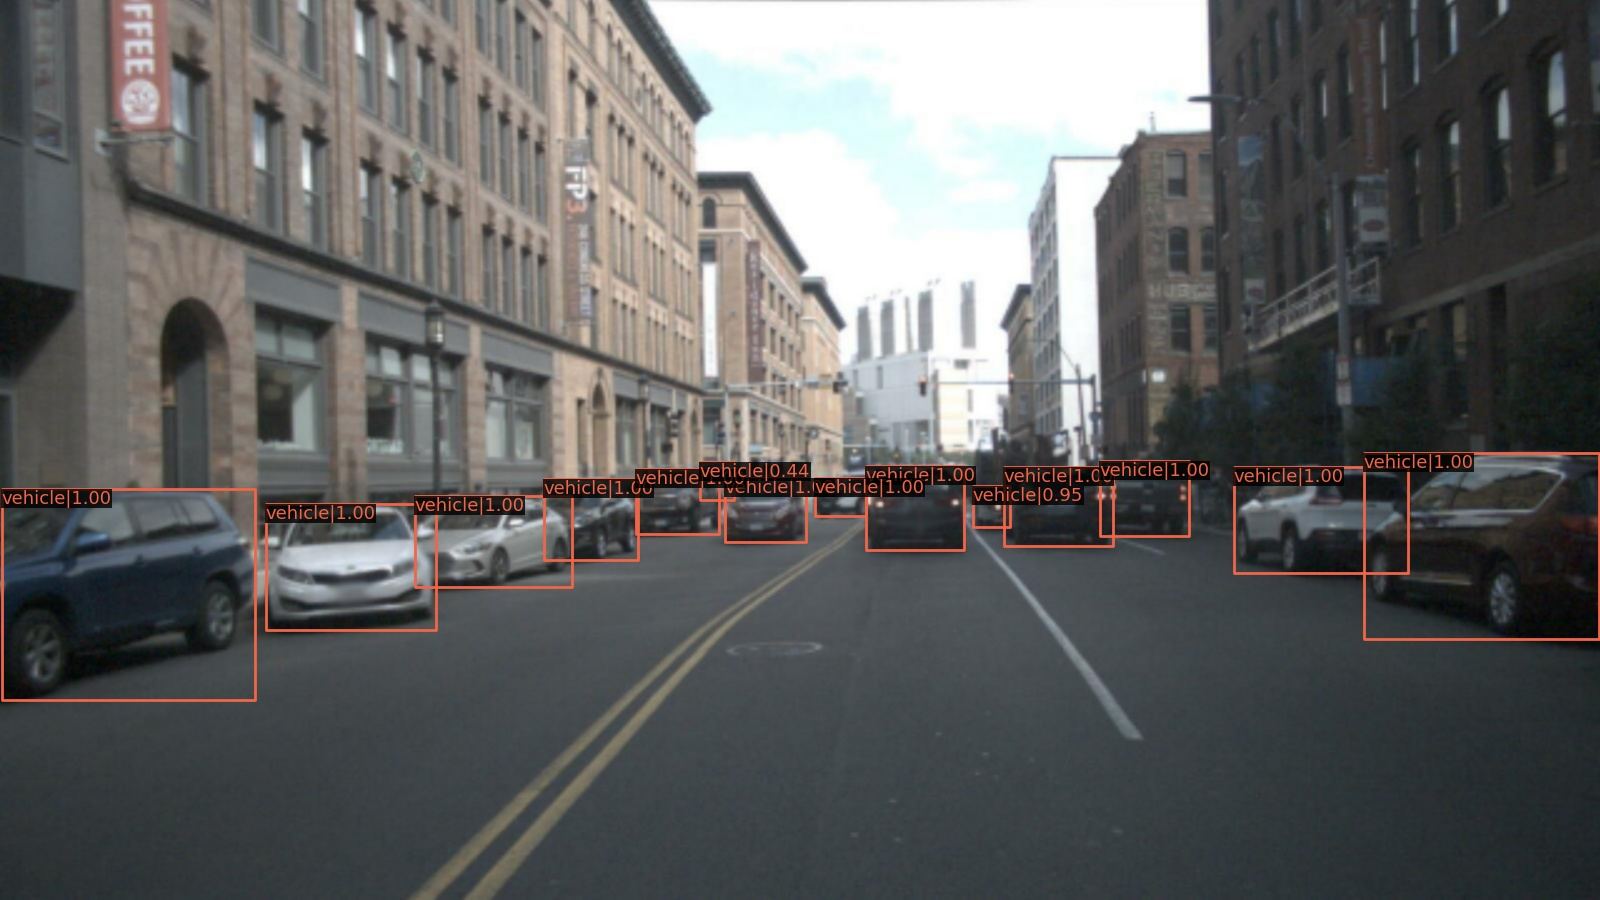
\includegraphics[width=0.3\textwidth]{images/results/saf_vs_hrfuser/samples/s3_day_regular/n008-2018-08-01-15-34-25-0400__CAM_FRONT__1533152655412404_former.jpg}
        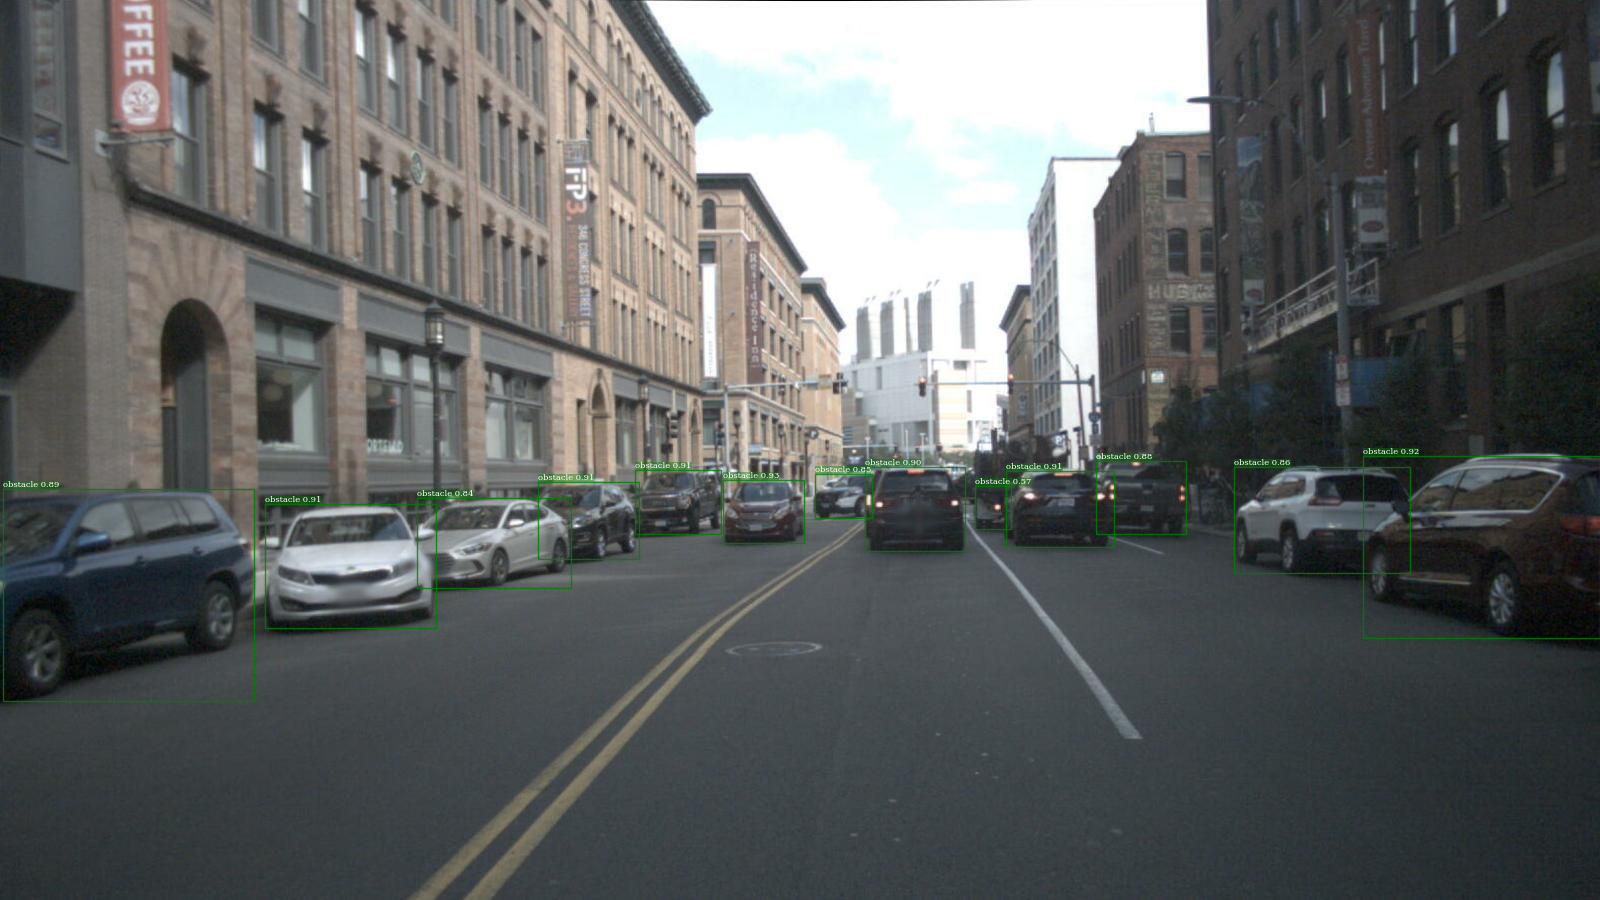
\includegraphics[width=0.3\textwidth]{images/results/saf_vs_hrfuser/samples/s3_day_regular/n008-2018-08-01-15-34-25-0400__CAM_FRONT__1533152655412404.png}
      
        % Row 2
        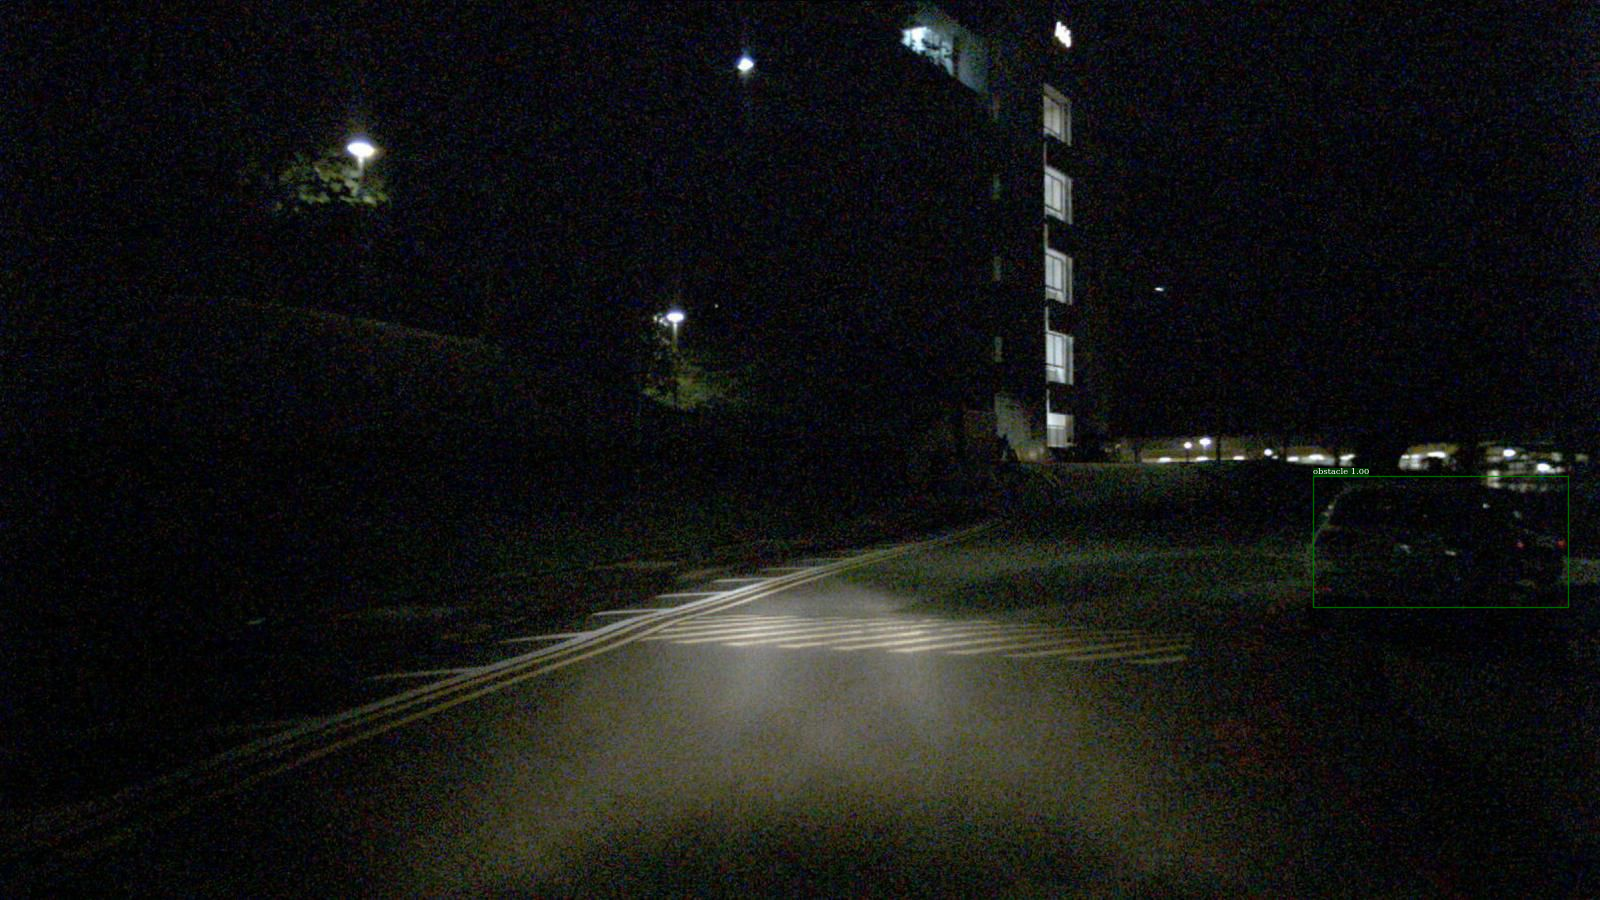
\includegraphics[width=0.3\textwidth]{images/results/saf_vs_hrfuser/samples/s4_night_reg/n015-2018-11-14-19-52-02+0800__CAM_FRONT__1542196675862460_gt.png}
        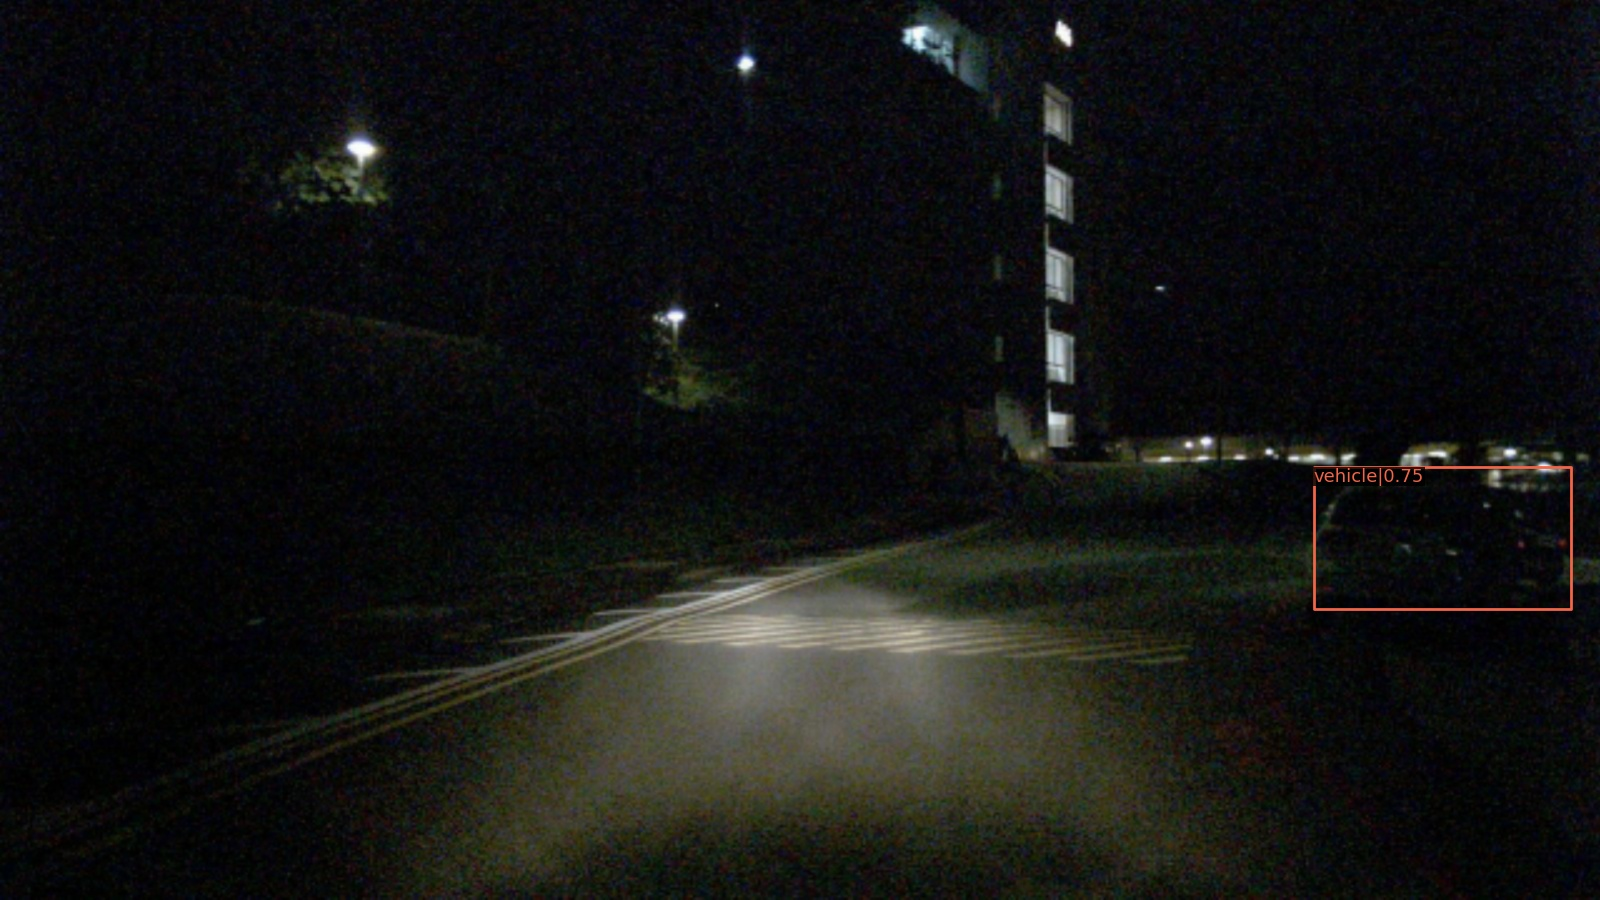
\includegraphics[width=0.3\textwidth]{images/results/saf_vs_hrfuser/samples/s4_night_reg/n015-2018-11-14-19-52-02+0800__CAM_FRONT__1542196675862460_former.jpg}
        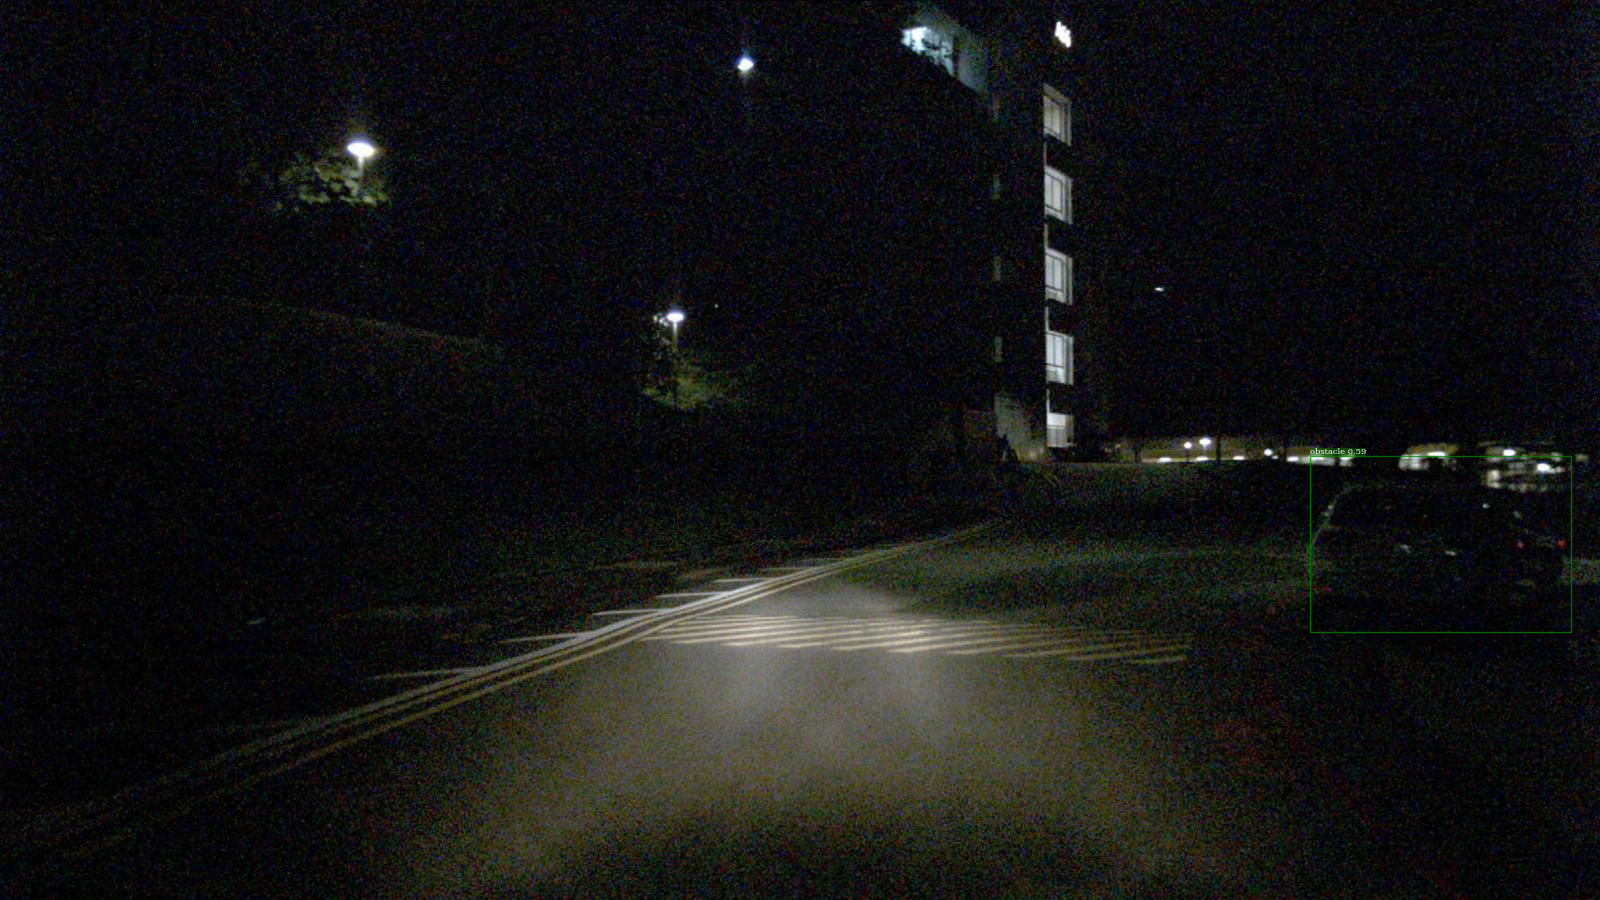
\includegraphics[width=0.3\textwidth]{images/results/saf_vs_hrfuser/samples/s4_night_reg/n015-2018-11-14-19-52-02+0800__CAM_FRONT__1542196675862460.png}
      
        % % Row 3
        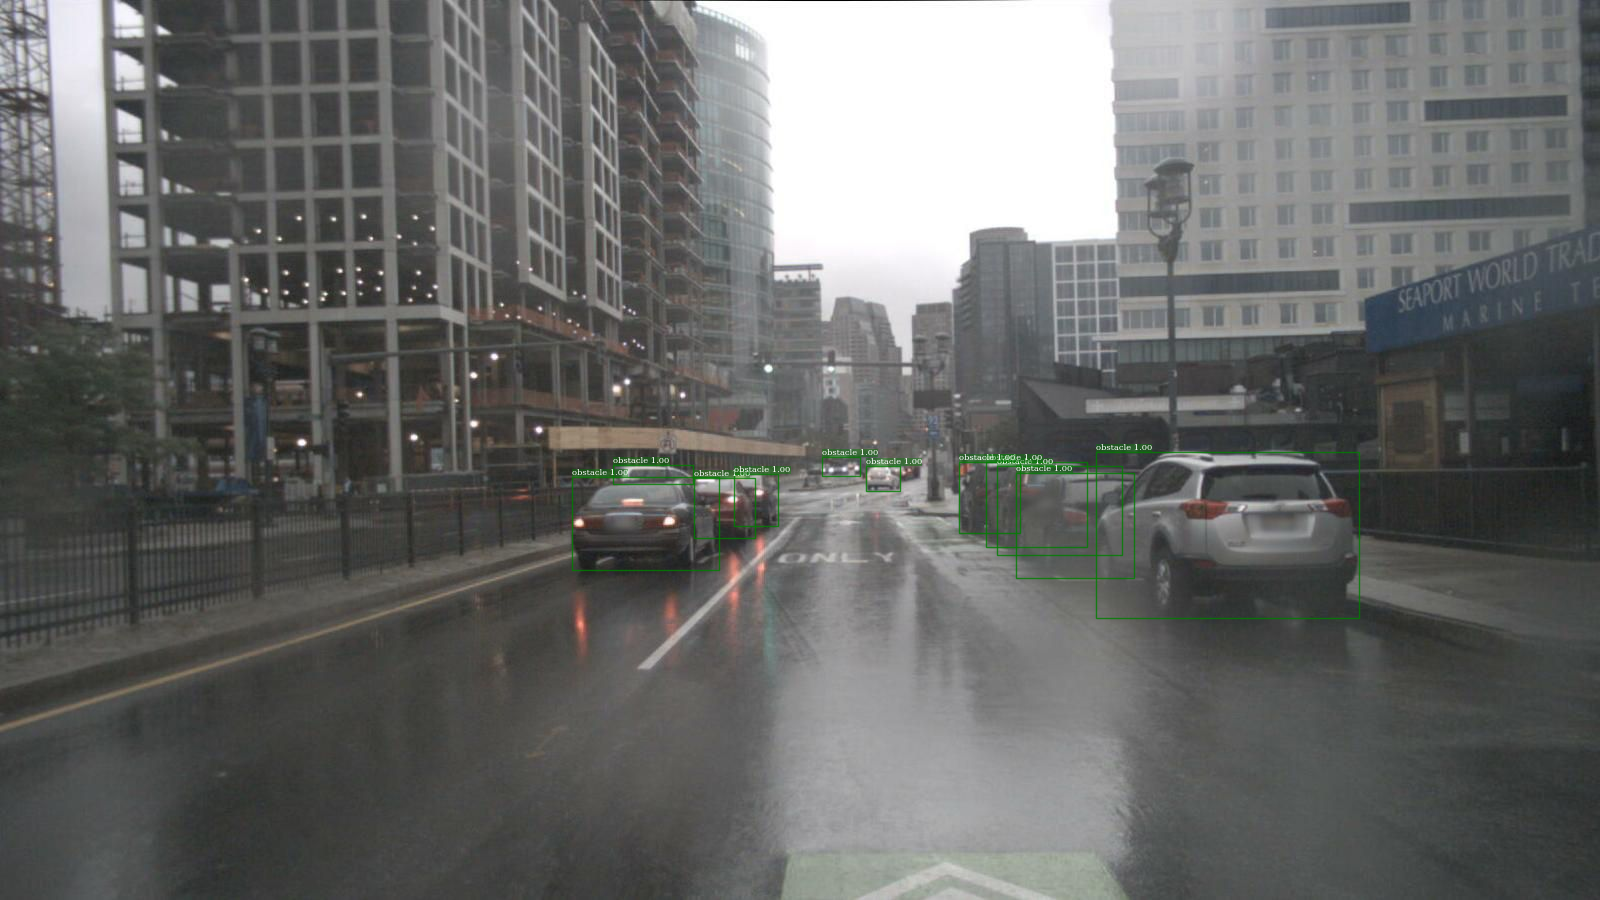
\includegraphics[width=0.3\textwidth]{images/results/saf_vs_hrfuser/samples/s5_rain_reg/n008-2018-09-18-14-18-33-0400__CAM_FRONT__1537295031112404_gt.png}
        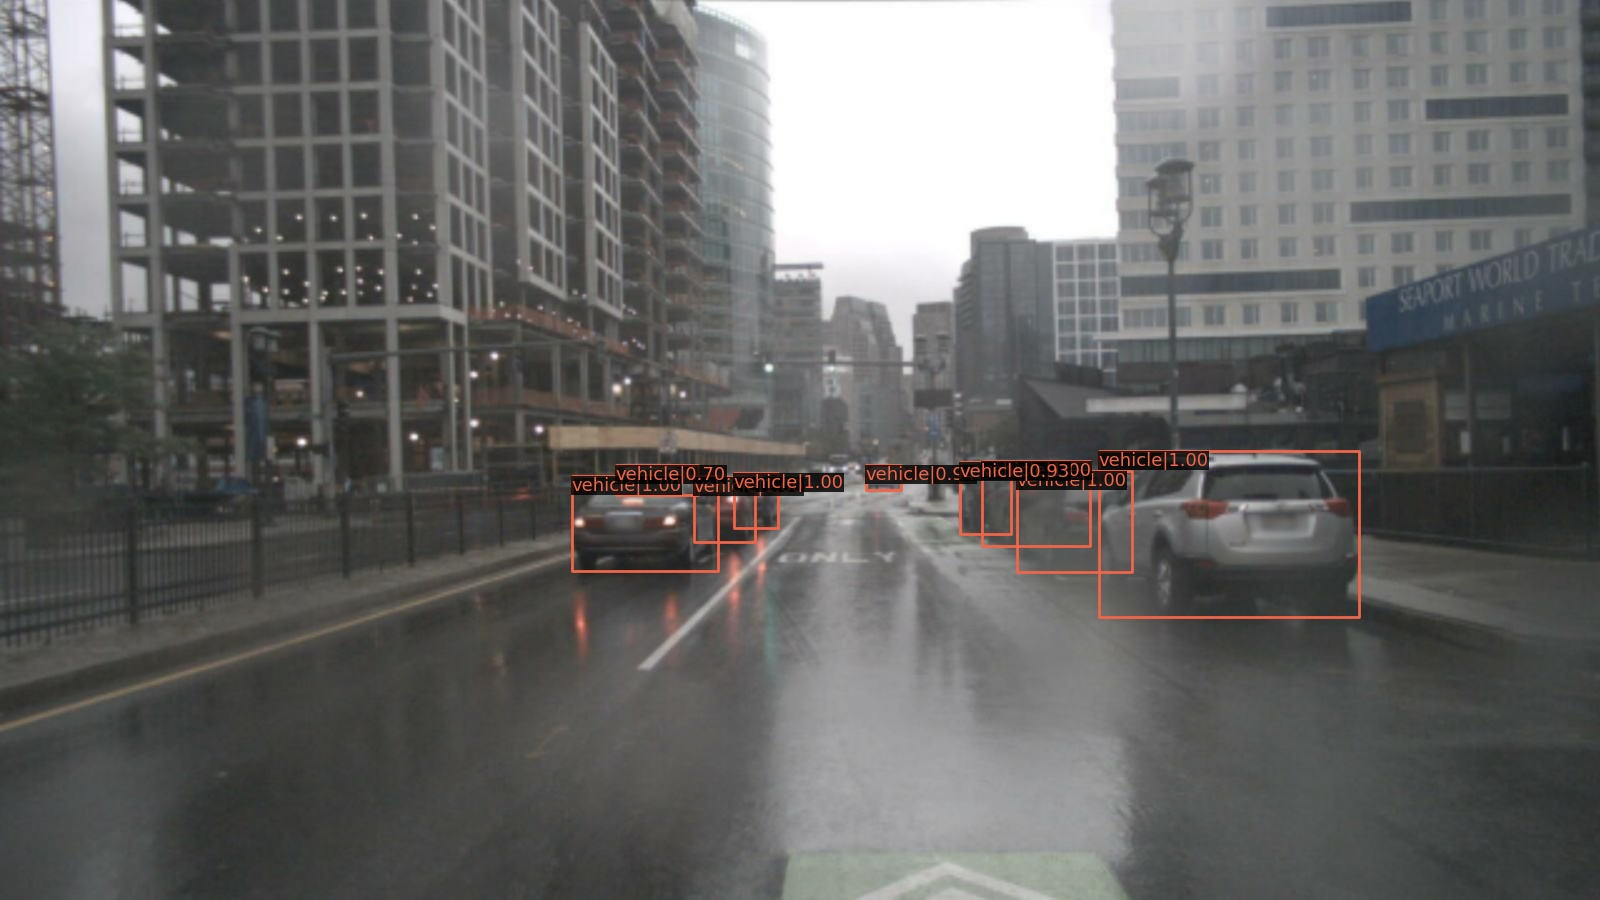
\includegraphics[width=0.3\textwidth]{images/results/saf_vs_hrfuser/samples/s5_rain_reg/n008-2018-09-18-14-18-33-0400__CAM_FRONT__1537295031112404_former.jpg}
        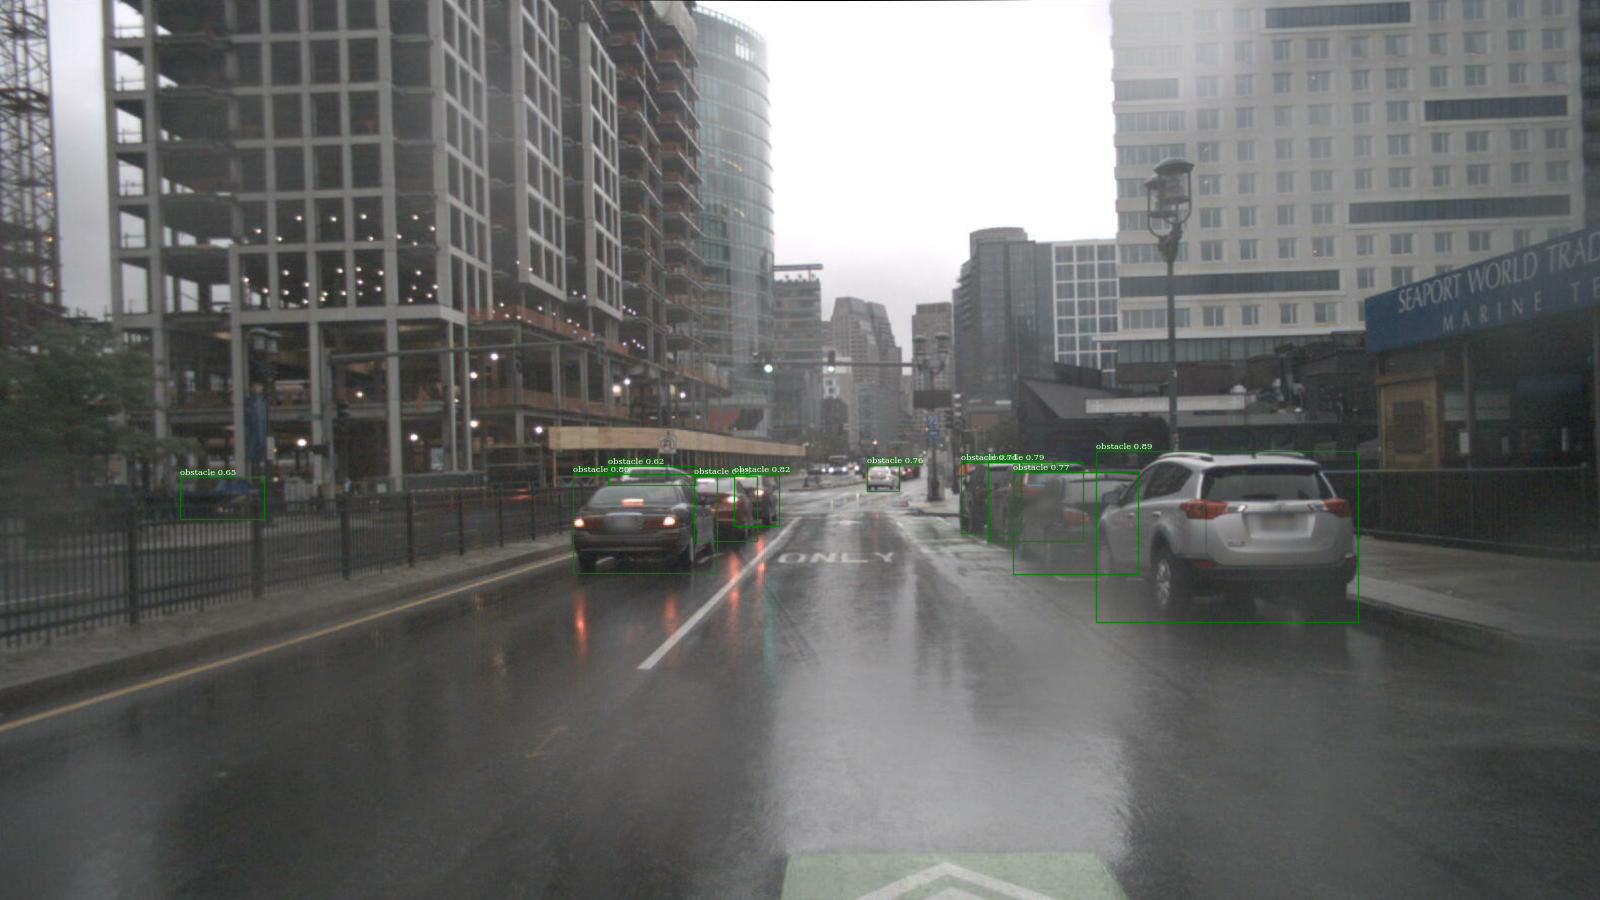
\includegraphics[width=0.3\textwidth]{images/results/saf_vs_hrfuser/samples/s5_rain_reg/n008-2018-09-18-14-18-33-0400__CAM_FRONT__1537295031112404.png}
      
        % % Row 4
        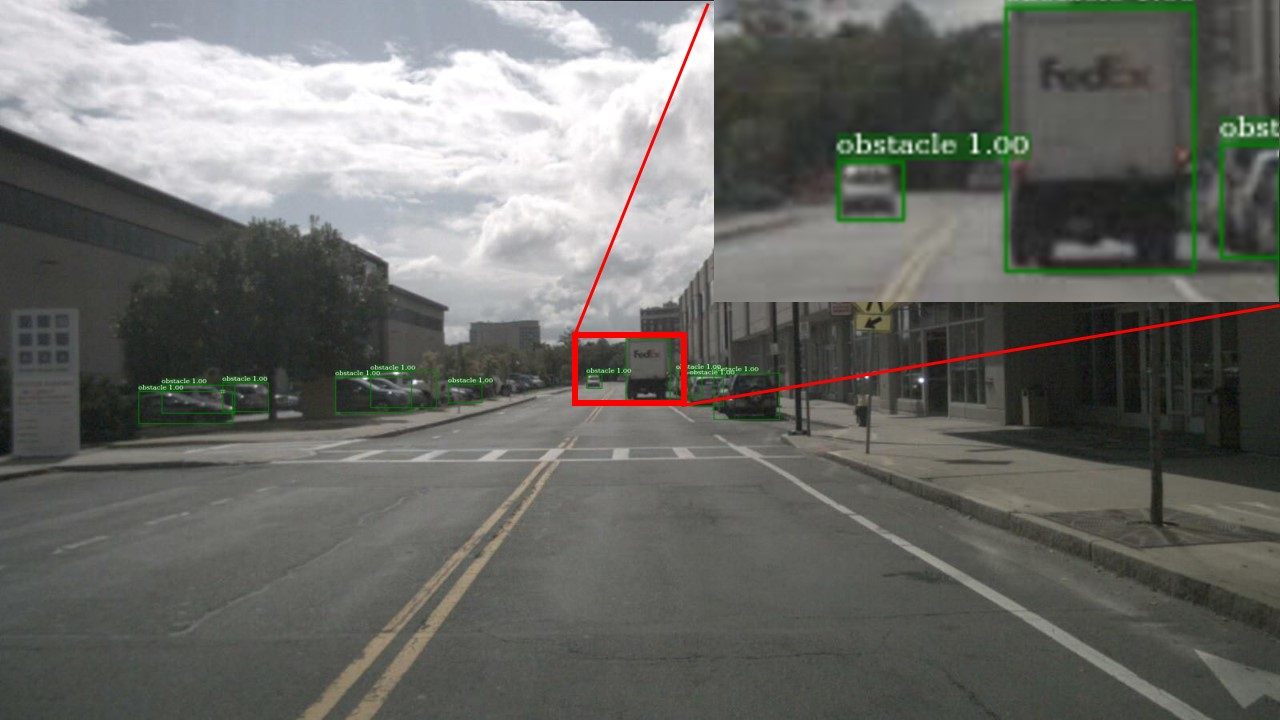
\includegraphics[width=0.3\textwidth]{images/results/saf_vs_hrfuser/samples/s1_small/n008-2018-08-01-15-34-25-0400__CAM_FRONT__1533152226912404_GT_2.jpg}
        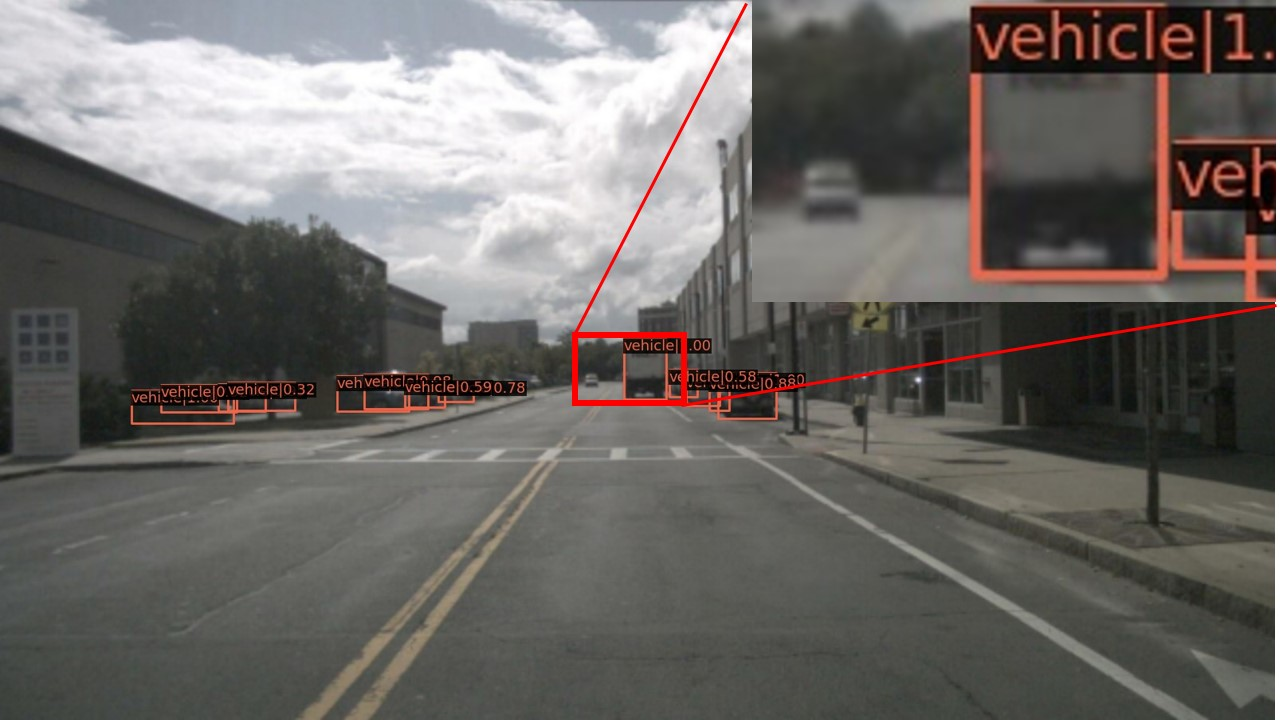
\includegraphics[width=0.3\textwidth]{images/results/saf_vs_hrfuser/samples/s1_small/n008-2018-08-01-15-34-25-0400__CAM_FRONT__1533152226912404_former_2.jpg}
        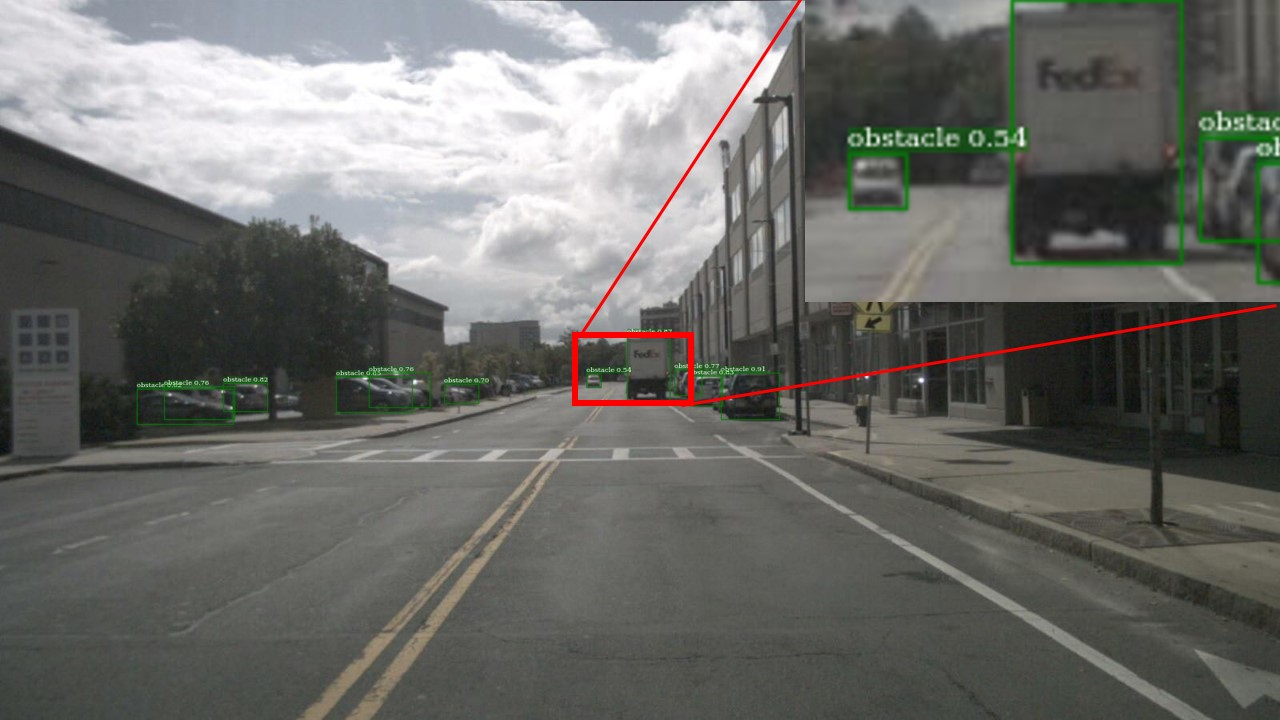
\includegraphics[width=0.3\textwidth]{images/results/saf_vs_hrfuser/samples/s1_small/n008-2018-08-01-15-34-25-0400__CAM_FRONT__1533152226912404_2.jpg}
      
        % % Row 5
        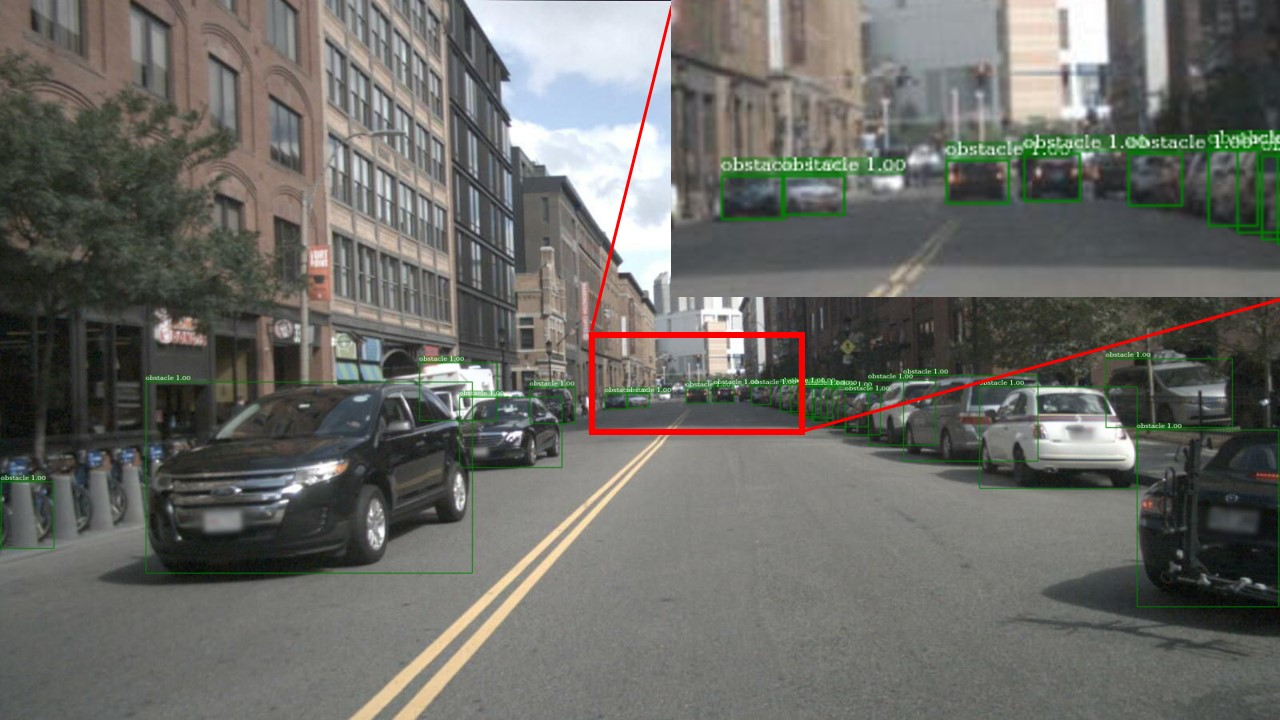
\includegraphics[width=0.3\textwidth]{images/results/saf_vs_hrfuser/samples/s2_small/n008-2018-08-01-15-34-25-0400__CAM_FRONT__1533152641412404_gt_2.jpg}
        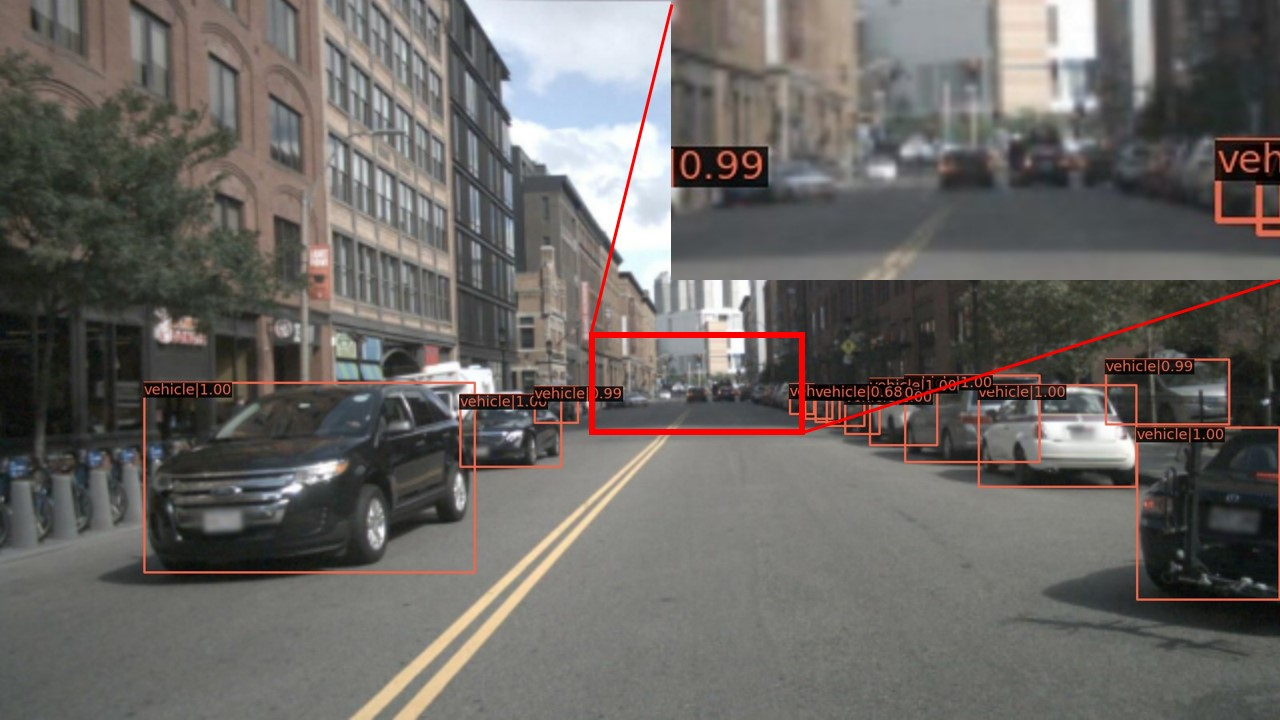
\includegraphics[width=0.3\textwidth]{images/results/saf_vs_hrfuser/samples/s2_small/n008-2018-08-01-15-34-25-0400__CAM_FRONT__1533152641412404_former_2.jpg}
        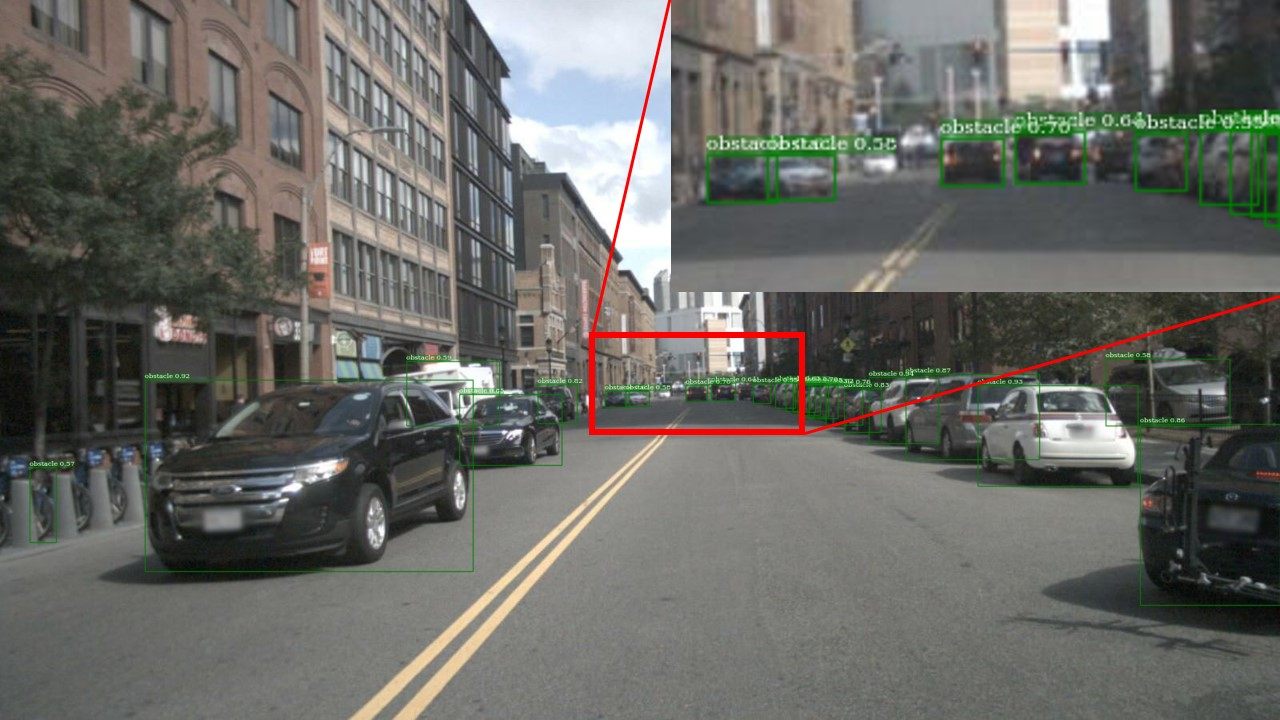
\includegraphics[width=0.3\textwidth]{images/results/saf_vs_hrfuser/samples/s2_small/n008-2018-08-01-15-34-25-0400__CAM_FRONT__1533152641412404_2.jpg}
      
        \caption{A few samples to showcase the detection results of HRFuser and SAF-FCOS. Where the 1st column is ground truth, 2nd is HRFuser, and 3rd is SAF-FCOS (1st Row: Day, 2nd Row: Night, 3rd Row: Rain, 4th and 5th Row: Small objects). Best viewed in zoomed-in view.}
        \label{fig:saf_vs_hrfuser}
      \end{figure}
    

    \subsection{Multimodal Sensor Fusion in HRFuser: Tightly-Coupled Fusion}

    % In this section, we compare importance of different sensors when it comes to detection in adverse weather conditions on the DENSE dataset. As discussed before, the DENSE dataset covers four different sensors for environment perception namely, Camera, Radar, LiDAR, and Gated infrared camera. Here, we are comparing how having complementary sensors improves the detection performance in challenging weather conditions. Both quantitative and qualitative analysis are presented in this section. Following are the comparison of only camera vs. camera+Radar vs. camera+LiDAR vs. camera+Radar+LiDAR and camera+Radar+LiDAR+gated infrared camera. The results are presented in accordance with COCO-style metrics, as outlined in Table \ref{tab:coco_metrics}.

    In this analysis, we delve into the significance of varying sensor combinations for object detection under adverse weather conditions, utilizing the DENSE dataset as our benchmark. The DENSE dataset, as previously mentioned, encompasses four distinct types of sensors for environmental perception: Camera, Radar, LiDAR, and a Gated infrared Camera. This comparison focuses on assessing the enhancement in detection performance brought about by the integration of these complementary sensors. We conduct both quantitative and qualitative evaluations, comparing scenarios using only a camera, camera combined with Radar, camera with LiDAR, a trio of camera, Radar, and LiDAR, and finally, an amalgamation of all four sensors including the gated infrared camera. For all experiments on HRFuser, only tightly-coupled fusion architecture is used. The results of these comparisons are meticulously analyzed using COCO-style metrics. This approach provides a comprehensive understanding of how each sensor contributes to the robustness of object detection in challenging weather conditions, underscoring the value of sensor fusion in enhancing environmental perception.

    The presented plots illustrate the impact of weather conditions, as represented on the x-axis. The DENSE dataset encompasses four distinct weather scenarios: Clear Weather, Light Fog, Dense Fog, and Snow/Rain. Within the dataset, each weather condition is further subdivided into 'Day' and 'Night' categories. This categorization is intended to demonstrate a model's performance under varying levels of ambient light. In the following plots, the transition between 'Day' and 'Night' for a specific weather condition is highlighted by the use of bold lines.

    \begin{figure}[h!]
        \centering
        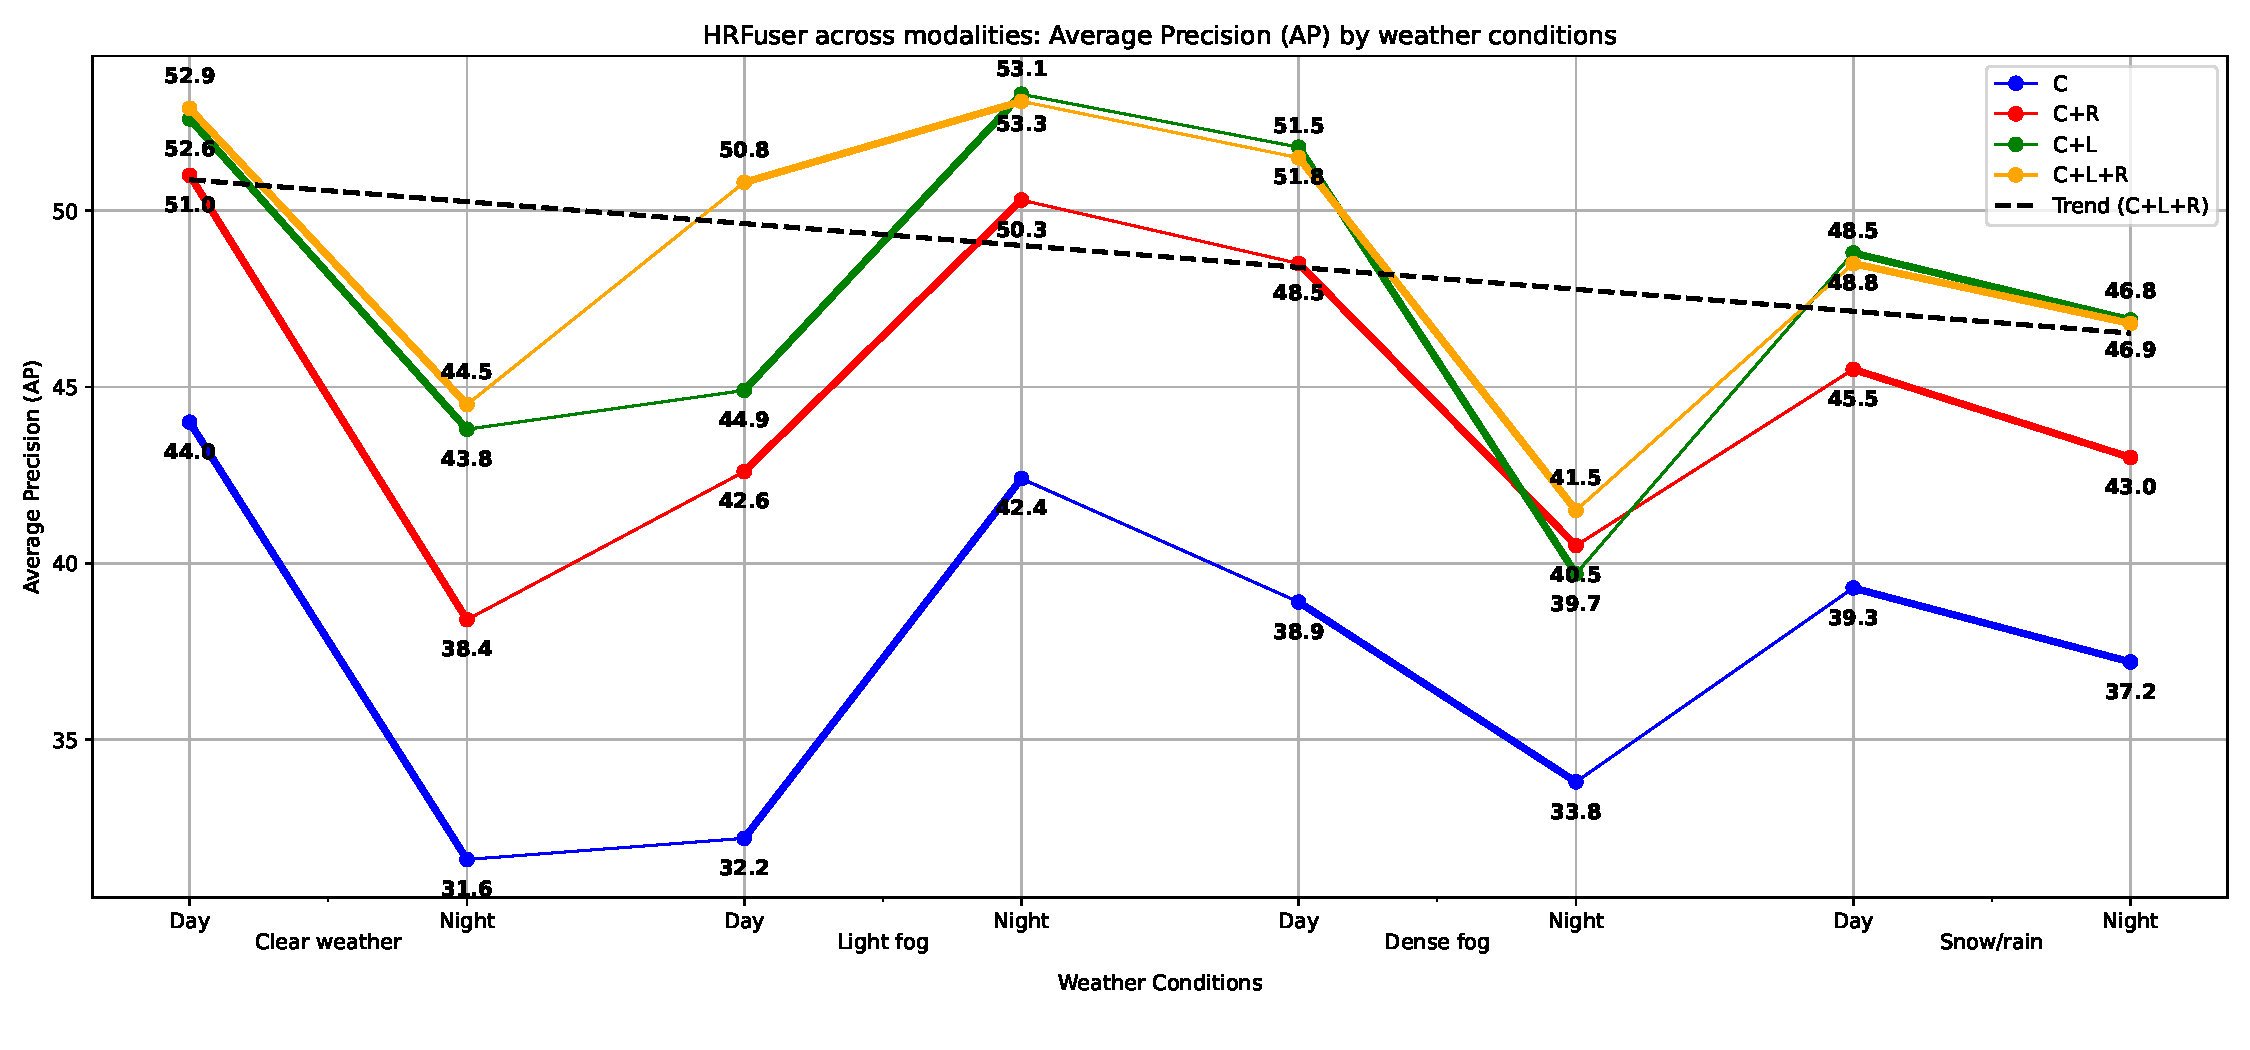
\includegraphics[width=1.0\textwidth]{images/results/hrfuser/ap.pdf}
        \caption{Performance of the HRFuser model in terms of Average Precision (AP) across various sensor modalities under different weather conditions. Note: C+L+R data point values are shown above the line and rest are below the line.}
        \label{fig:hrfuser_ap}
    \end{figure}

    \begin{figure}[]
        \centering
        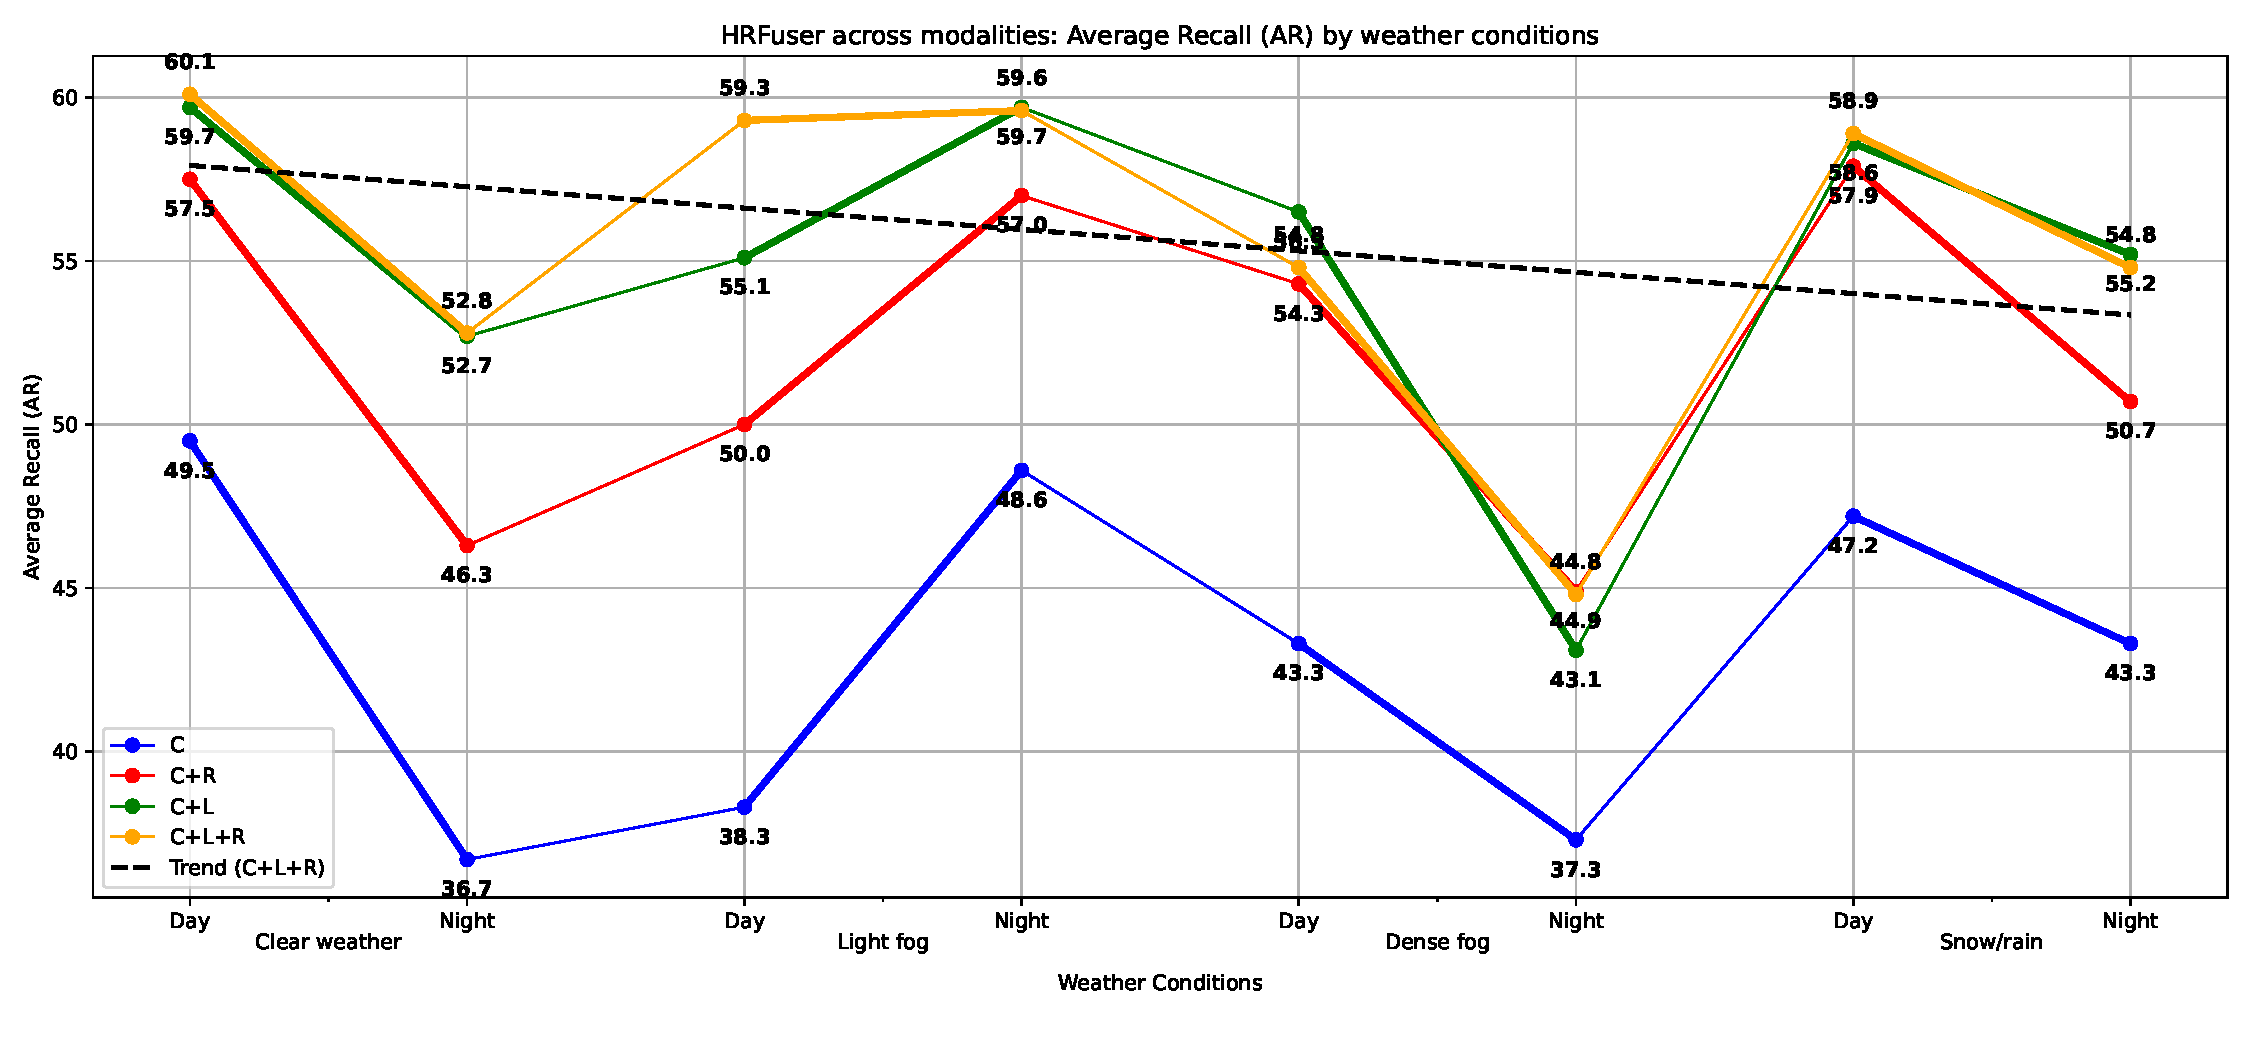
\includegraphics[width=1.0\textwidth]{images/results/hrfuser/ar.pdf}
        \caption{Performance of the HRFuser model in terms of Average Recall (AR) across various sensor modalities under different weather conditions. Note: C+L+R data point values are shown above the line and rest are below the line.}
        \label{fig:hrfuser_ar}
    \end{figure}

    % The graph provides insights into the balance between computational load and efficiency for varying combinations of sensors.
    \begin{figure}[h!]
        \centering
        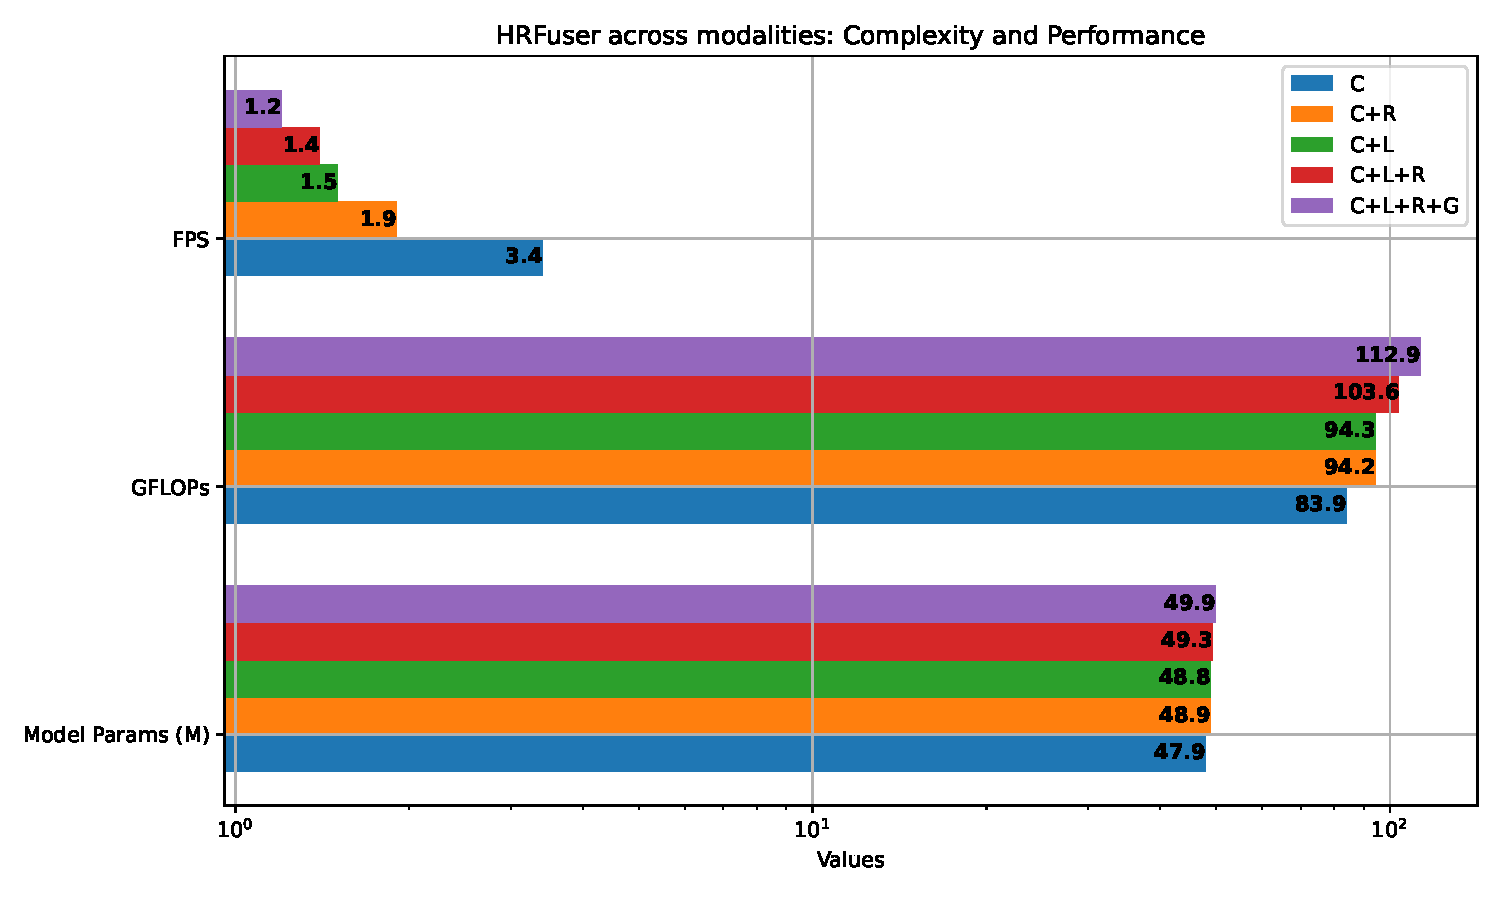
\includegraphics[width=0.8\textwidth]{images/results/hrfuser/model_complexity.pdf}
        \caption{HRFuser model's complexity and performance, displayed through model parameters (in M), GFLOPs, and FPS, across different sensor modalities. Note: this is a common plot with an additional modality, Gated infrared camera.}
        \label{fig:hrfuser_model_complexity}
    \end{figure}



    % Points:
    % - shows day vs night highlighted with bold line, except light fog, there is trend from day to night performance reduction probably due to camera low light
    % - trendline shows the performance of perception system from clear to adverse weather declination
    % - observe that in dense fog, camera+Radar performs better than camera+LiDAR, mainly due to LiDAR points affecting by fog,  
    % - across all modalities, camera+Radar+LiDAR tops the list, shows the clear advantage fusion of complementary sensors 
    % - only camera performs worst across all modalities
    % - both AP and AR follows the same trend
    The analysis highlights a distinct shift in the performance of the perception system from day to night, marked by a bold line. This trend, barring a light fog, suggests a performance reduction during nighttime, likely attributed to the camera's low-light limitations. Additionally, the trendline indicates a gradual decline in system efficiency from clear to adverse weather conditions. Ideally, the trendline should be straight to showcase the same the performance of the perception system in different weather conditions. Interestingly, in dense fog scenarios, the combination of camera and Radar outperforms camera and LiDAR. This is primarily due to the LiDAR points being adversely affected by fog. When evaluating all modalities, the fusion of camera, Radar, and LiDAR emerges as the most effective, underscoring the benefits of integrating complementary sensors. In contrast, systems relying solely on camera technology exhibit the lowest performance across all tested modalities. Moreover, both Average Precision (AP) and Average Recall (AR) metrics demonstrate a consistent trend, aligning with the overall observations of sensor performance under varying conditions.

    \subsubsection{With an Additional Modality}
    
    Incorporating a gated infrared camera into the HRFuser model significantly enhances its performance in terms of Average Precision (AP) and Average Recall (AR). As depicted in the model complexity and performance chart (referenced as \ref{fig:hrfuser_model_complexity}), this additional modality results in only a minimal increase in model parameters by 1.22\% and an 8.98\% increment in GFLOPs, while maintaining a negligible drop in frames per second (fps). Consequently, the combination of camera, Radar, LiDAR, and gated infrared camera emerges as the top performer across all modalities. Notably, the gated infrared camera demonstrates reduced impact under adverse weather conditions, a fact quantitatively supported by the data in Table \ref{table:quantitative_effect_of_weather}. However, its effectiveness is not extensively tested across a variety of scenarios due to its limited availability in the majority of the dataset. This finding further indicates that HRFuser is capable of handling an arbitrary number of modalities within the same model framework, as discussed in the relevant section.

    \begin{figure}[]
        \centering
        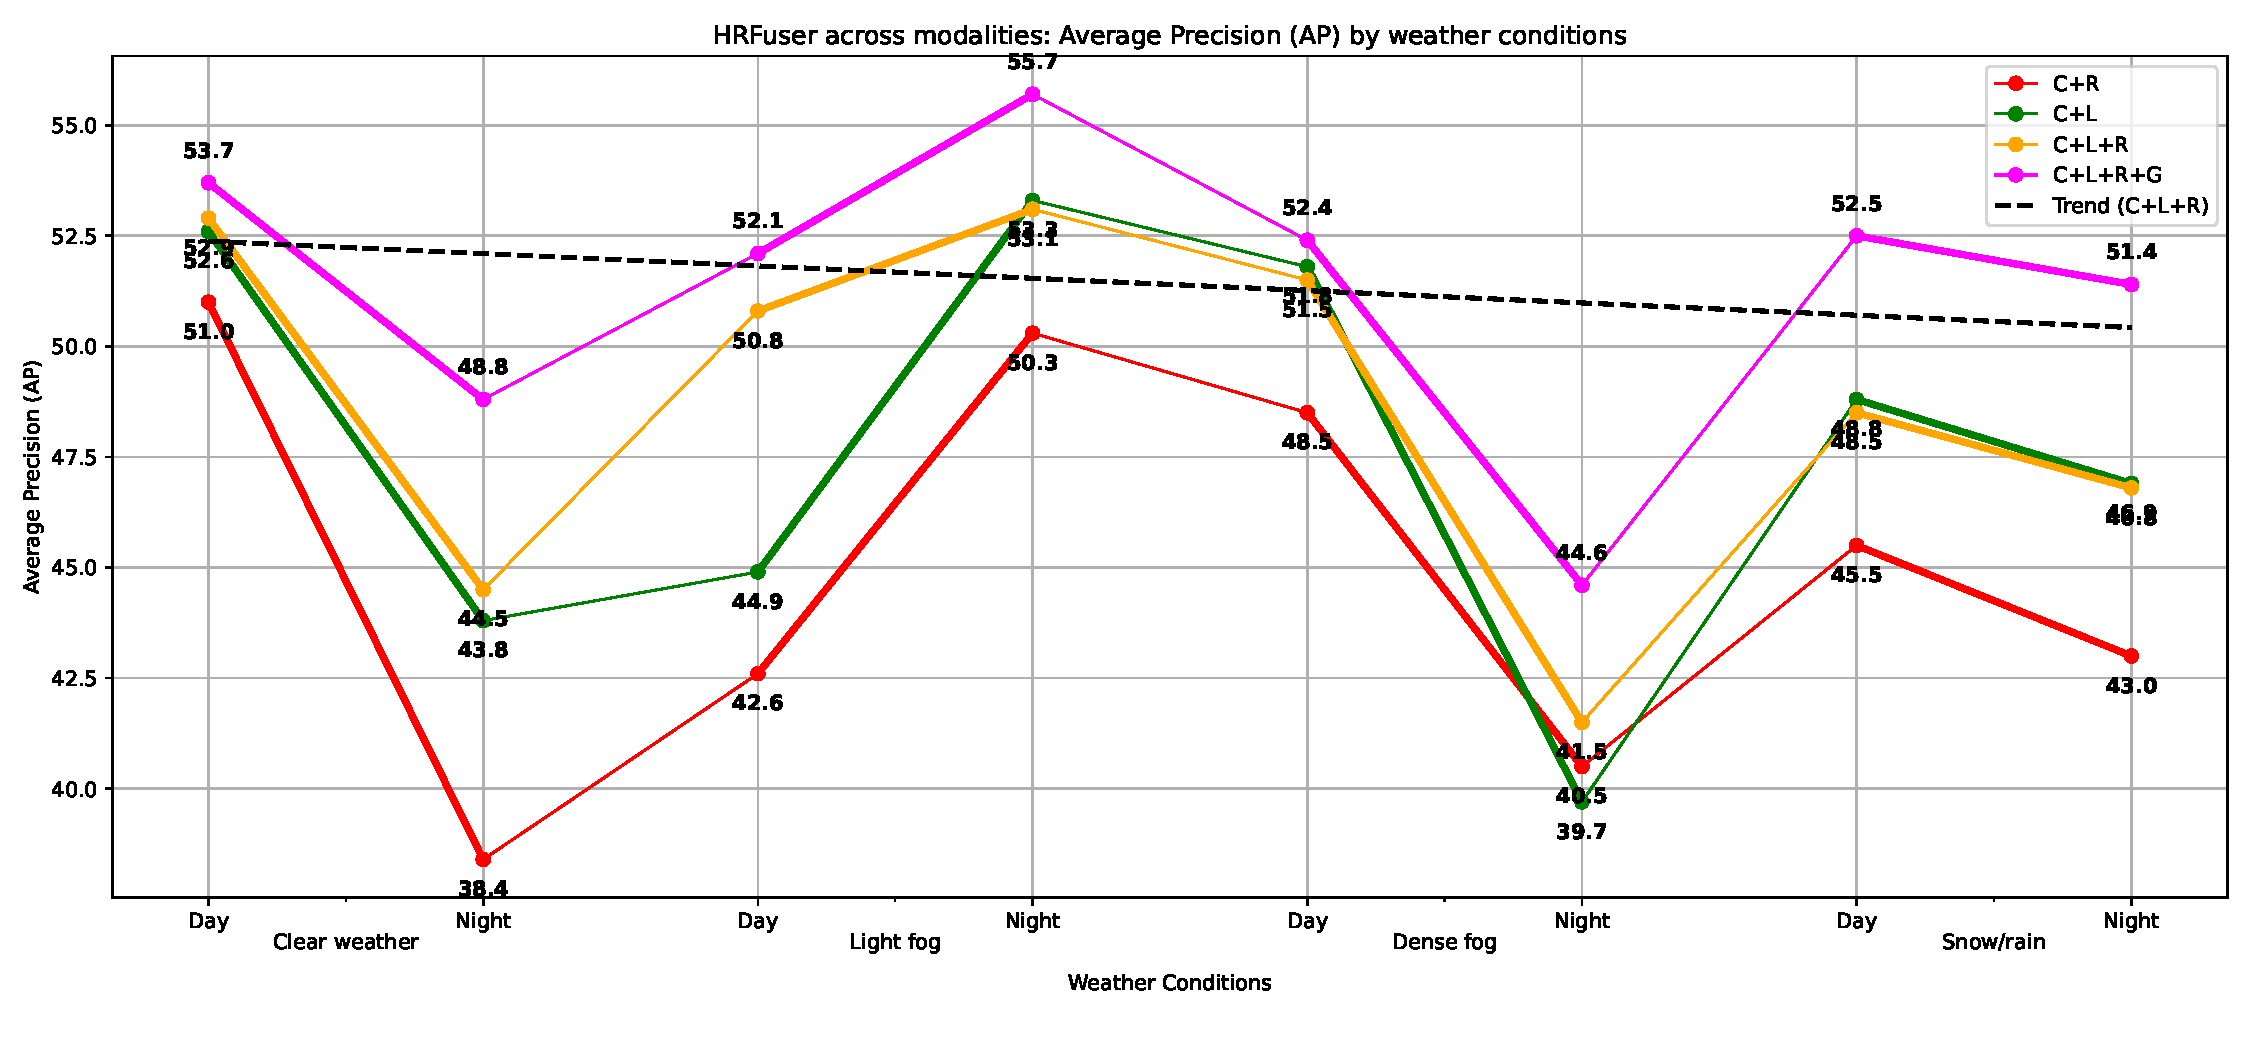
\includegraphics[width=1.0\textwidth]{images/results/hrfuser/additional_modality/ap_2.pdf}
        \caption{Performance of the HRFuser model in terms of Average Precision (AP) across various sensor modalities under different weather conditions with an additional sensor Gated infrared camera. Note: C+L+R data point values are shown above the line and rest are below the line.}
        \label{fig:hrfuser_ap_2}
    \end{figure}

    \begin{figure}[]
        \centering
        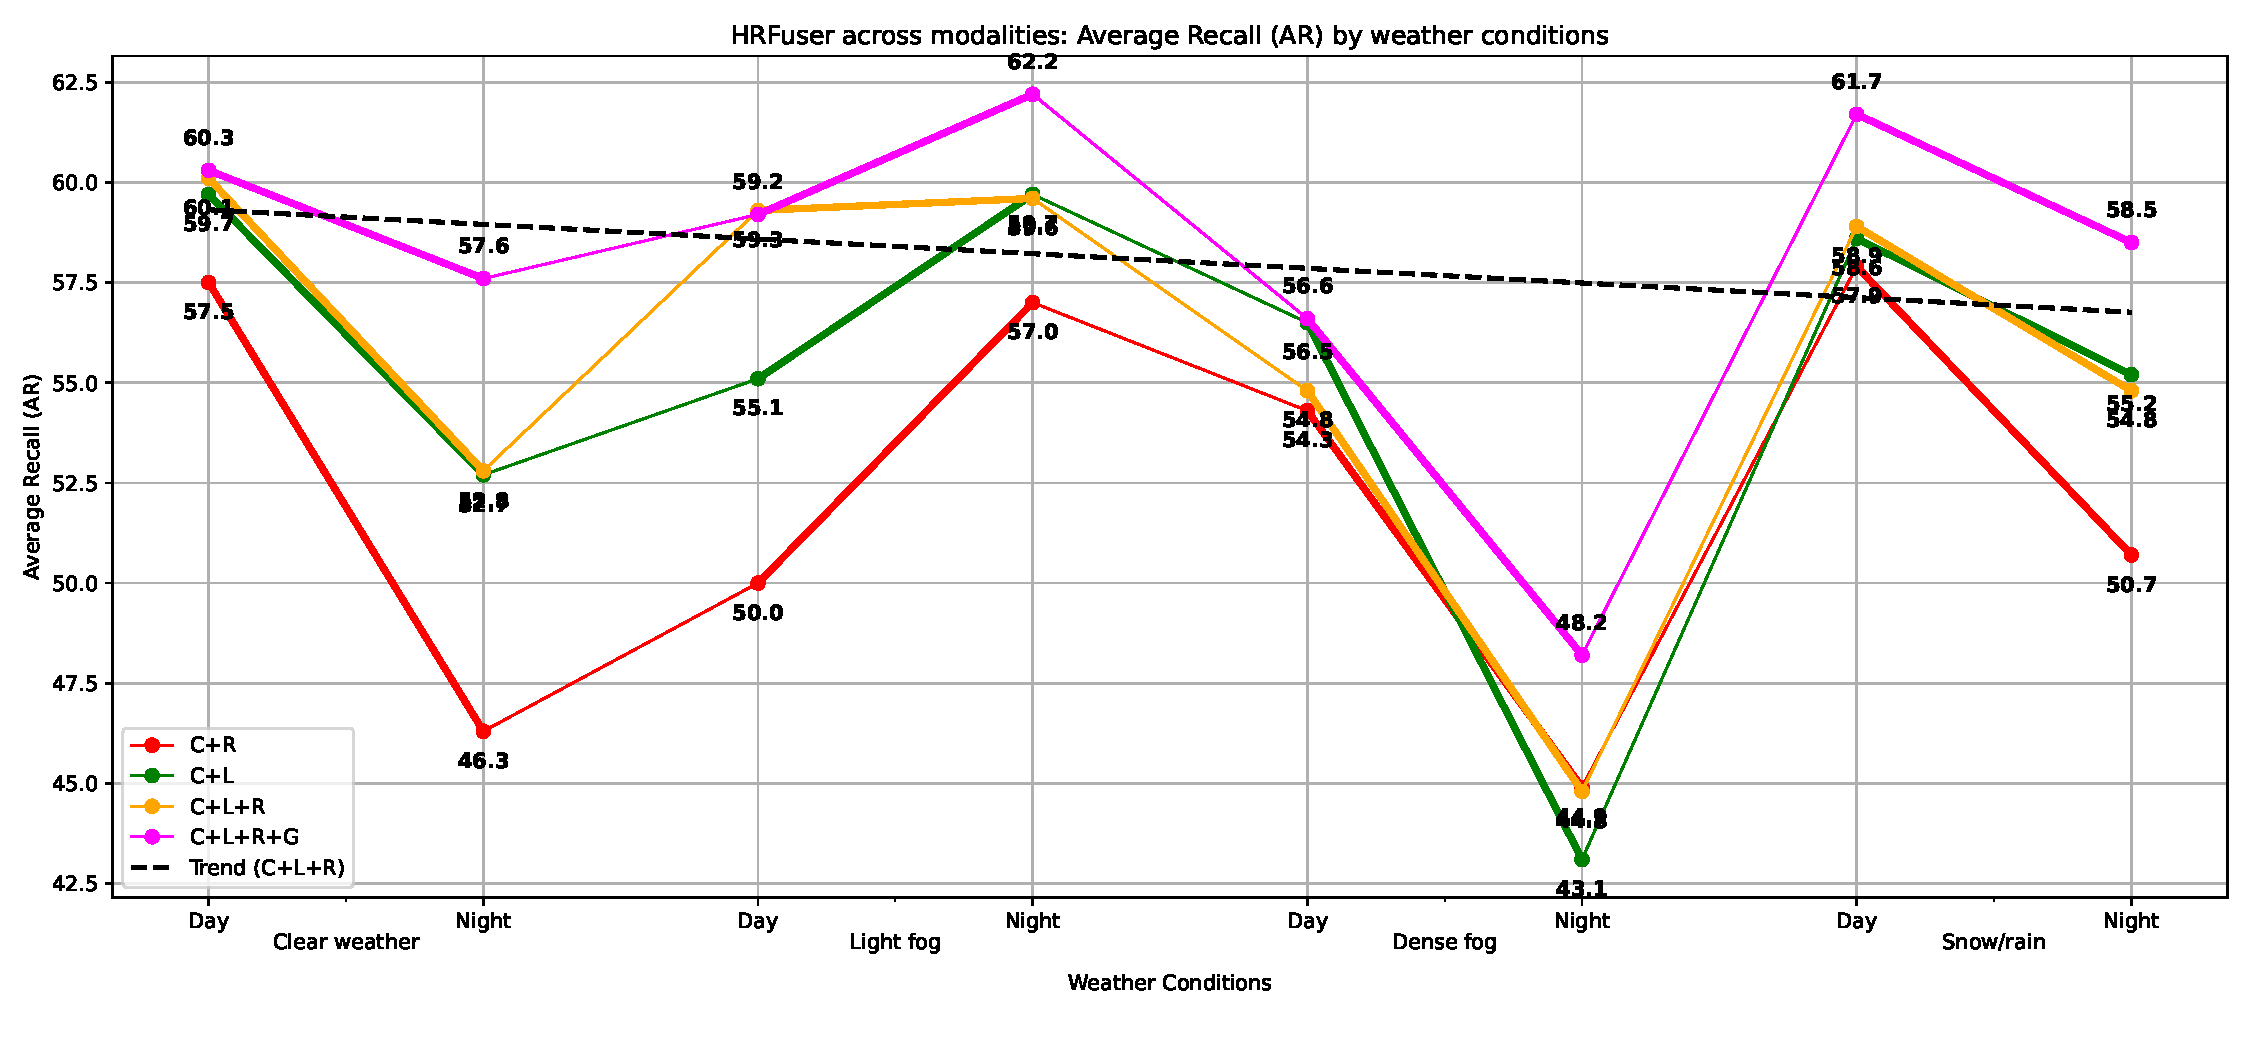
\includegraphics[width=1.0\textwidth]{images/results/hrfuser/additional_modality/ar_2.pdf}
        \caption{Performance of the HRFuser model in terms of Average Recall (AR) across various sensor modalities under different weather conditions with an additional sensor Gated infrared camera. Note: C+L+R data point values are shown above the line and rest are below the line.}
        \label{fig:hrfuser_ar_2}
    \end{figure}

    \paragraph*{Qualitative Analysis: Comparison across Modalities}

    In the DENSE adverse weather dataset, we present samples that emphasize the critical role of multimodal sensors in achieving robust perception under adverse weather conditions. Figure \ref{fig:hrfuser_on_dense} below illustrates the detection results comparing the Camera-only model to the multimodal C+L+R-based Tightly-Coupled Fusion model.

    The data presented in the figure corroborates the findings of the preceding quantitative analysis. Specifically, the camera-only model demonstrates a limitation in object detection under adverse weather conditions, attributed to decreased visibility. In contrast, the multimodal sensor fusion model, which integrates data from various complementary sensors, shows remarkable efficacy in object detection even under challenging conditions. It is noteworthy that all models were initially trained in clear weather scenarios and had no prior exposure to extreme weather conditions. The success of the multimodal model in these situations can be attributed to its feature fusion strategy at multiple levels, utilizing input from diverse sensors. Consequently, when one sensor's effectiveness is compromised due to environmental factors, the other robust sensors compensate, ensuring reliable object detection. This ability to adapt and perform accurately under varied conditions underscores the significant advantage of the multimodal Tightly-Coupled Fusion architecture in object detection tasks.

    \begin{figure}[h!]
        \centering
        % Row 1
        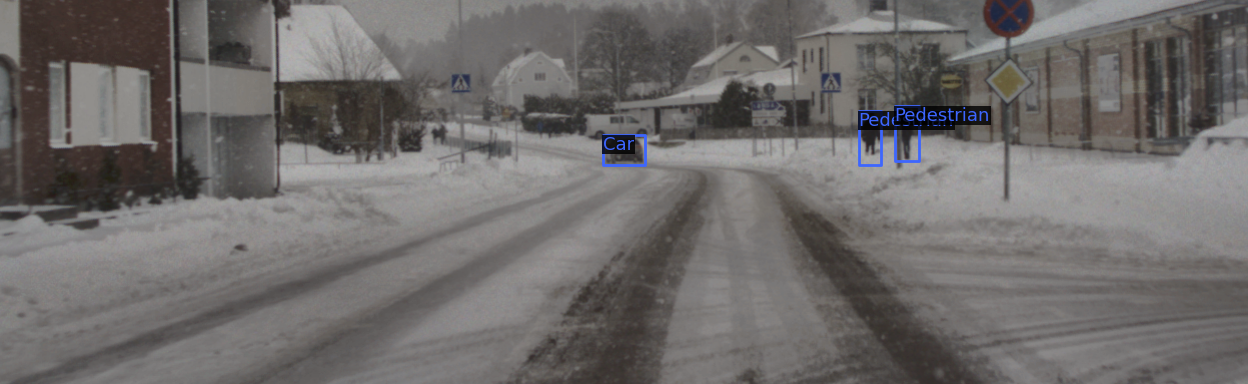
\includegraphics[width=0.3\textwidth]{images/results/hrfuser/samples/day_snow/2018-02-07_11-54-15_00440.png}
        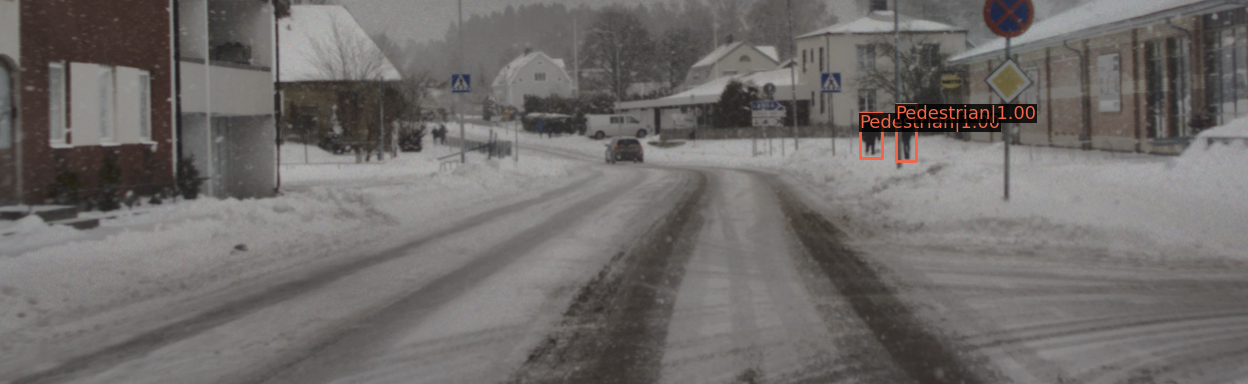
\includegraphics[width=0.3\textwidth]{images/results/hrfuser/samples/day_snow/2018-02-07_11-54-15_00440_former_c.png}
        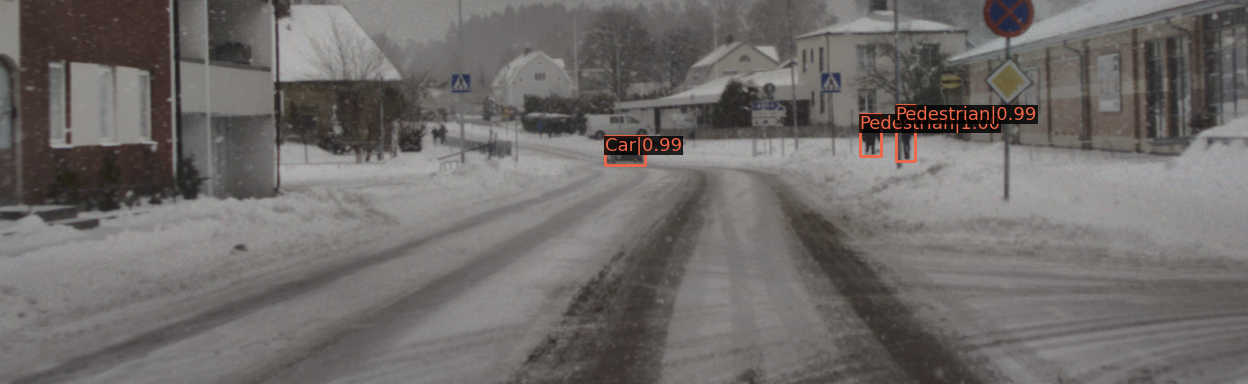
\includegraphics[width=0.3\textwidth]{images/results/hrfuser/samples/day_snow/2018-02-07_11-54-15_00440_former_clr.png}
      
        % Row 2
        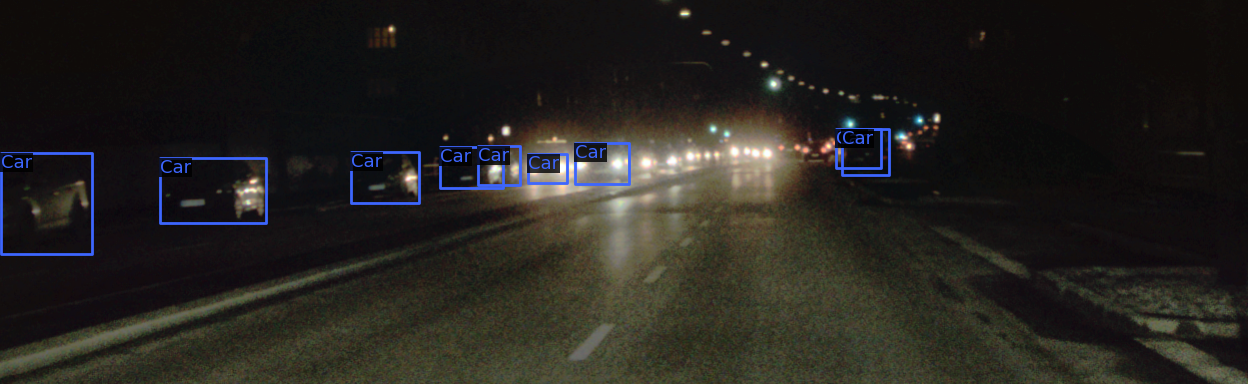
\includegraphics[width=0.3\textwidth]{images/results/hrfuser/samples/clear_night/2018-02-04_18-18-20_00100_gt.png}
        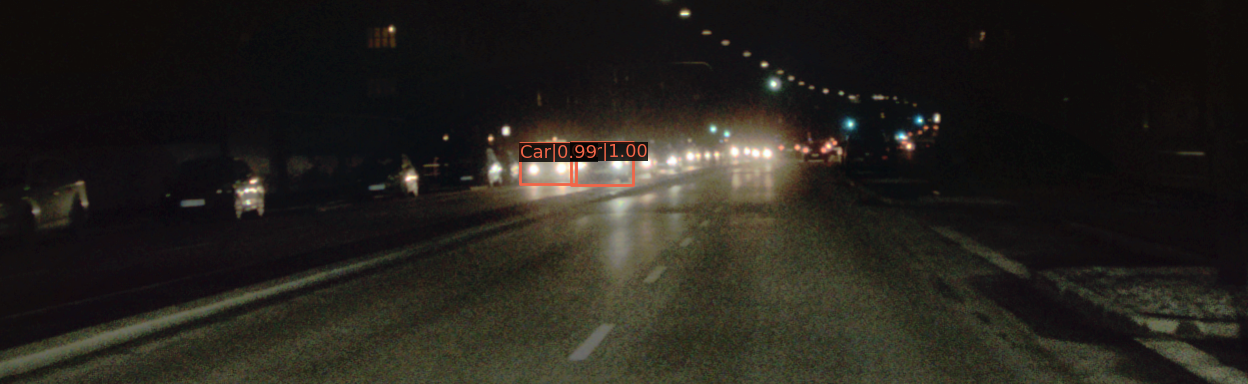
\includegraphics[width=0.3\textwidth]{images/results/hrfuser/samples/clear_night/2018-02-04_18-18-20_00100_former_c.png}
        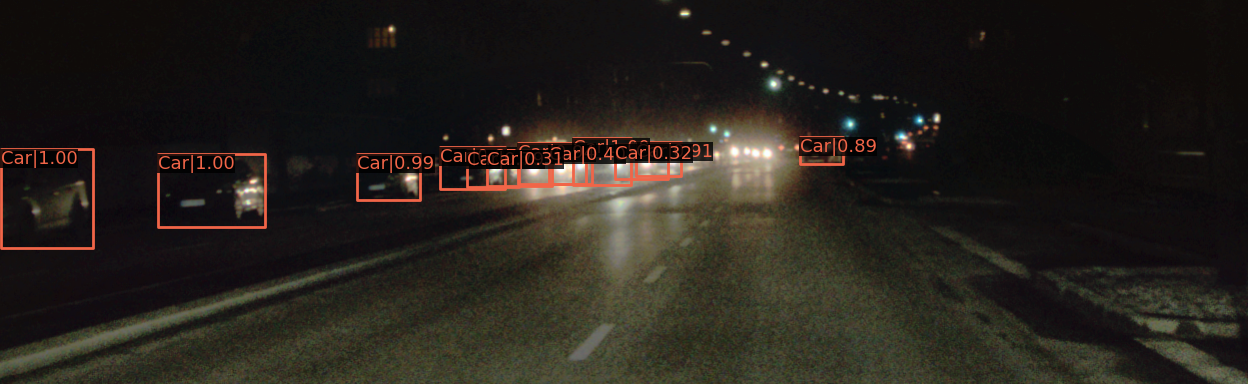
\includegraphics[width=0.3\textwidth]{images/results/hrfuser/samples/clear_night/2018-02-04_18-18-20_00100_former_clr.png}
      
        % % Row 3
        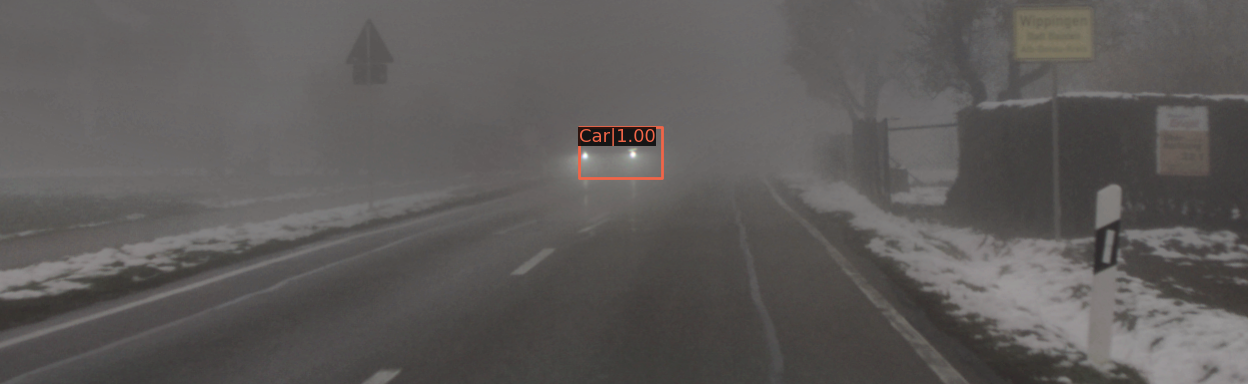
\includegraphics[width=0.3\textwidth]{images/results/hrfuser/samples/dense_fog_camera_fails/2018-10-29_15-02-37_00900_gt.png}
        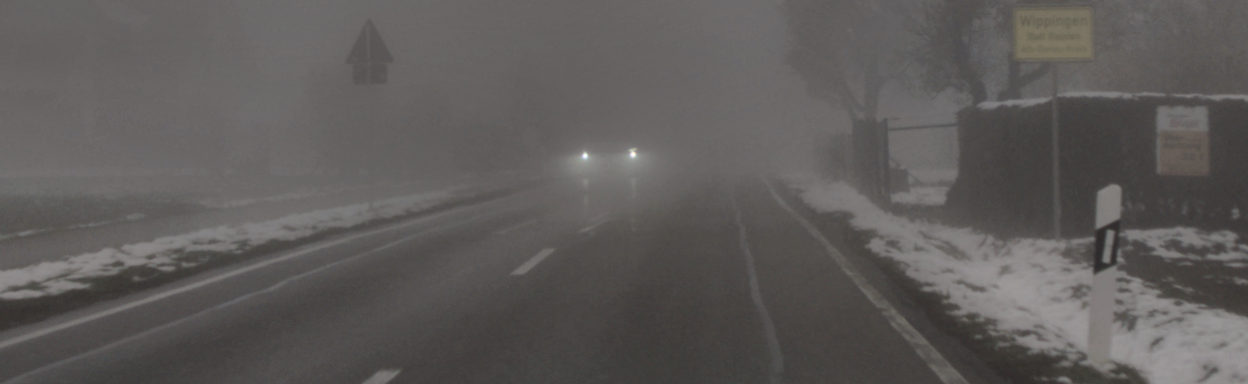
\includegraphics[width=0.3\textwidth]{images/results/hrfuser/samples/dense_fog_camera_fails/2018-10-29_15-02-37_00900_former.png}
        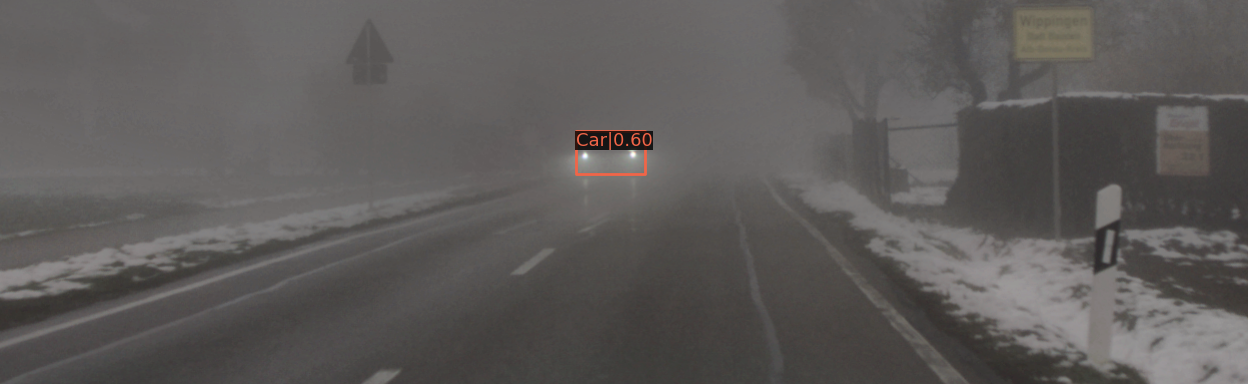
\includegraphics[width=0.3\textwidth]{images/results/hrfuser/samples/dense_fog_camera_fails/2018-10-29_15-02-37_00900_former_clr.png}
      
        % % Row 4
        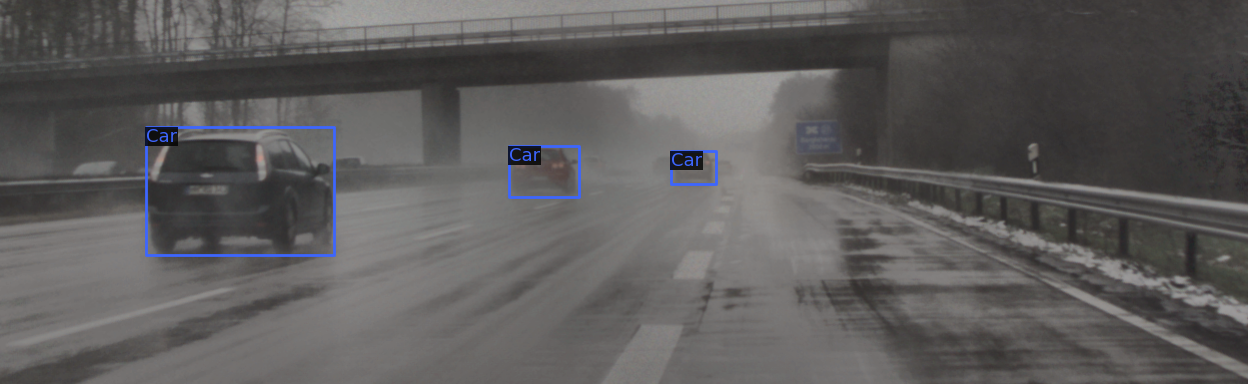
\includegraphics[width=0.3\textwidth]{images/results/hrfuser/samples/light_fog_day/2018-02-04_13-26-00_00100_gt.png}
        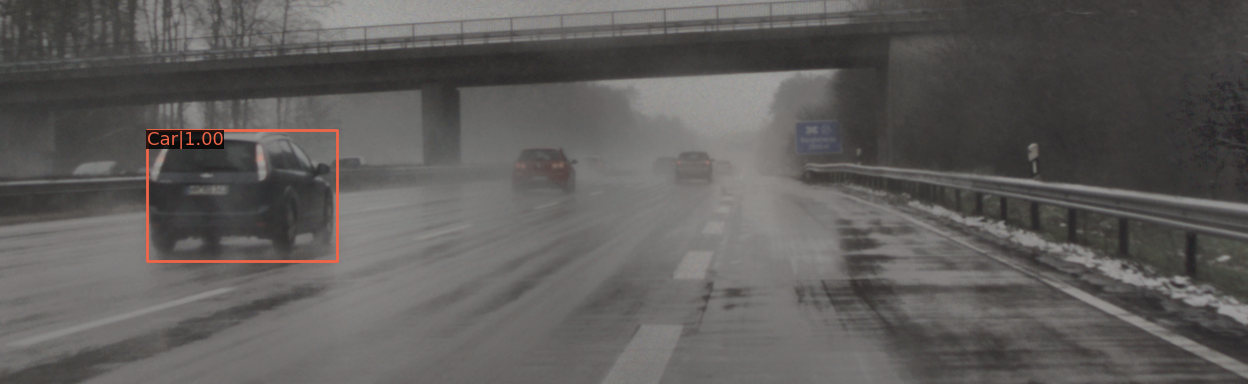
\includegraphics[width=0.3\textwidth]{images/results/hrfuser/samples/light_fog_day/2018-02-04_13-26-00_00100_former_c.png}
        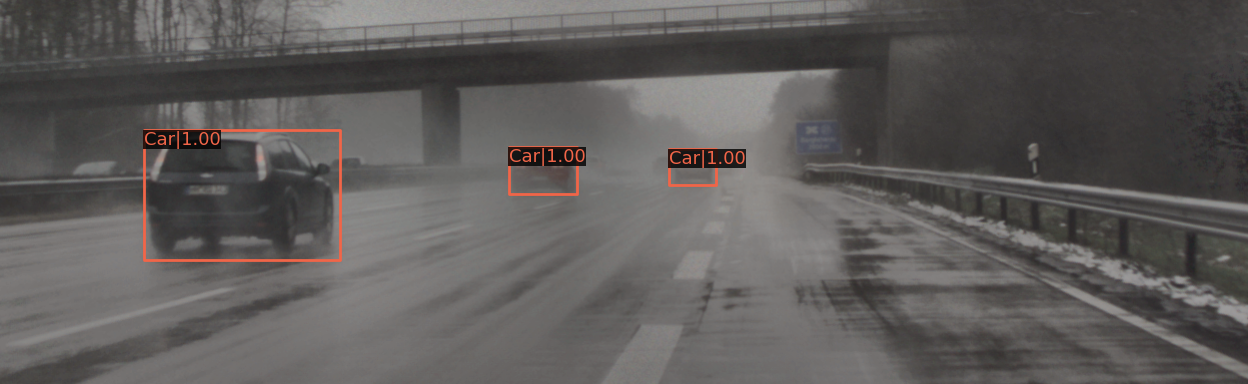
\includegraphics[width=0.3\textwidth]{images/results/hrfuser/samples/light_fog_day/2018-02-04_13-26-00_00100_former_clr.png}
      
        % % Row 5
        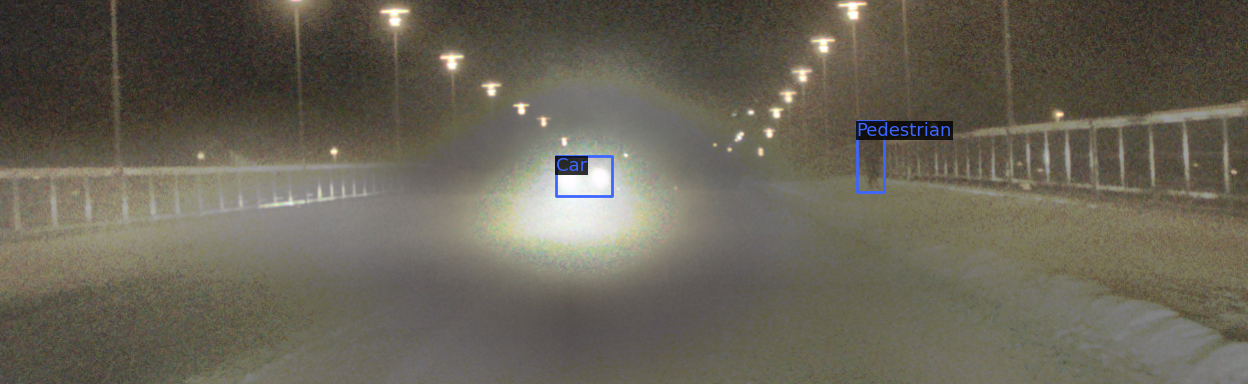
\includegraphics[width=0.3\textwidth]{images/results/hrfuser/samples/dense_fog_night/2018-02-07_17-56-35_00110.png}
        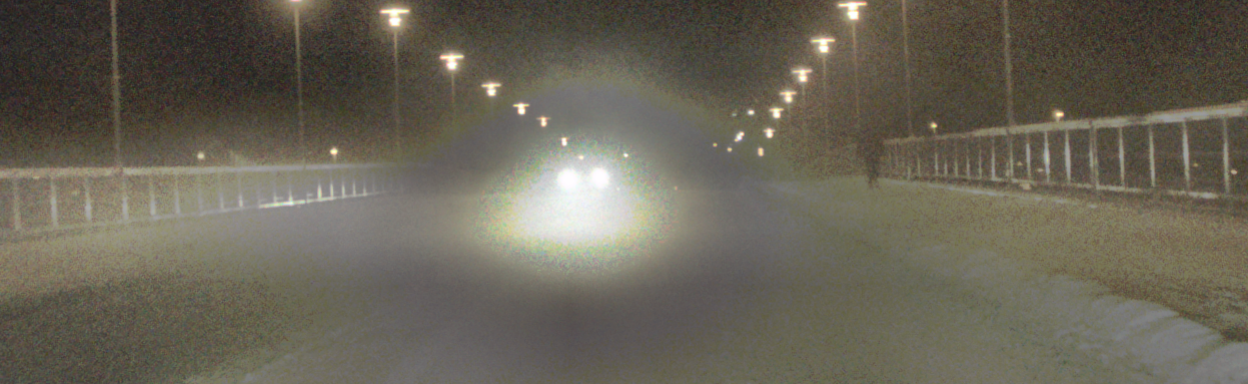
\includegraphics[width=0.3\textwidth]{images/results/hrfuser/samples/dense_fog_night/2018-02-07_17-56-35_00110_former_c.png}
        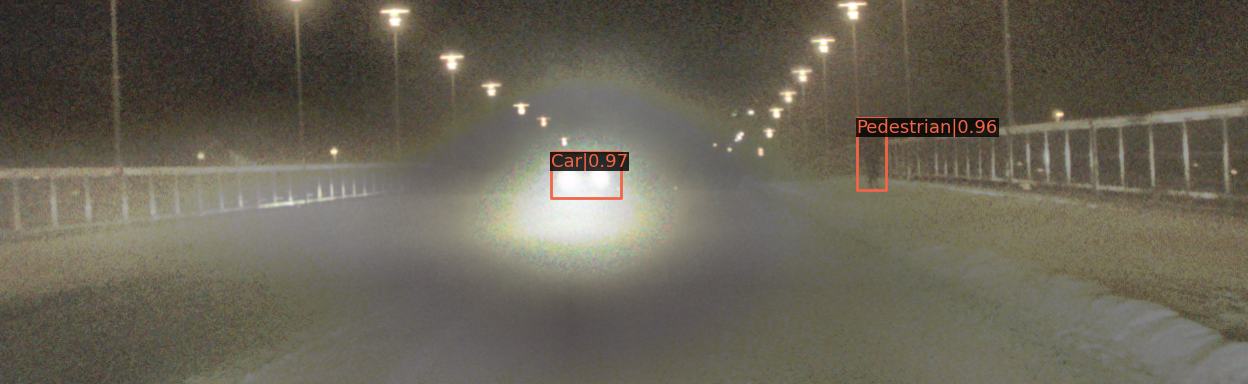
\includegraphics[width=0.3\textwidth]{images/results/hrfuser/samples/dense_fog_night/2018-02-07_17-56-35_00110_former_clr.png}
      
        \caption{A few samples to showcase the detection results of HRFuser. Where the 1st column is ground truth, 2nd is Camera only, and 3rd is Tightly-Coupled Fusion with C+L+R (Rows show the challenging weather conditions). Best viewed in zoomed-in view.}
        \label{fig:hrfuser_on_dense}
      \end{figure}
    
    

    \FloatBarrier
    \subsection{Multimodal Sensor Fusion in MT-DETR: Spanning Early to Tightly-Coupled Fusion}

    Here, experiments are conducted to compare the different modalities with MT-DETR method on the DENSE dataset. As MT-DETR also provides various configurations for its architecture, the experiments are conducted on the following fusion architecture configurations: 'Early', 'Middle', and 'Tightly-coupled' with all available sensors in the dataset. The experiment covers comparison among different combinations of sensors: Camera only (C), Camera+LiDAR (C+L), Camera+Radar (C+R) and Camera+LiDAR+Radar (C+L+R). In the following plots, the Camera only (C) results are without any fusion, it is a single modality experiment.

    Note that Average Recall (AR) plots are not shown below as they are following the same data trend as Average Precision (AP) plots. 

    In the model complexity plots presented, Frames Per Second (FPS) data are not included. We tested only one configuration on the V100 GPU, which is the MT-DETR Tightly-Coupled Fusion with C+L+R modalities, achieving 1.4 FPS. Other combinations were not tested on the V100 due to time and computational limitations. All model evaluations were conducted on a high-end A100 GPU to facilitate faster computation. However, this difference in hardware used for inference, compared to other methods, means that the results are not directly comparable.

    \FloatBarrier
    \subsubsection{Early Fusion: C vs. C+R vs. C+L+R}

    The accompanying plots illustrate the performance of the MT-DETR Early Fusion model. It is evident that the 'Camera only' mode outperforms other fusion modalities, particularly in adverse weather conditions. This superior performance can be attributed to the nature of Early Fusion, which is significantly influenced by the quality of input sensor raw data. If one of the sensors fails to detect accurately, it leads to challenges in subsequent feature extraction stages.

        \begin{figure}[]
            \centering
            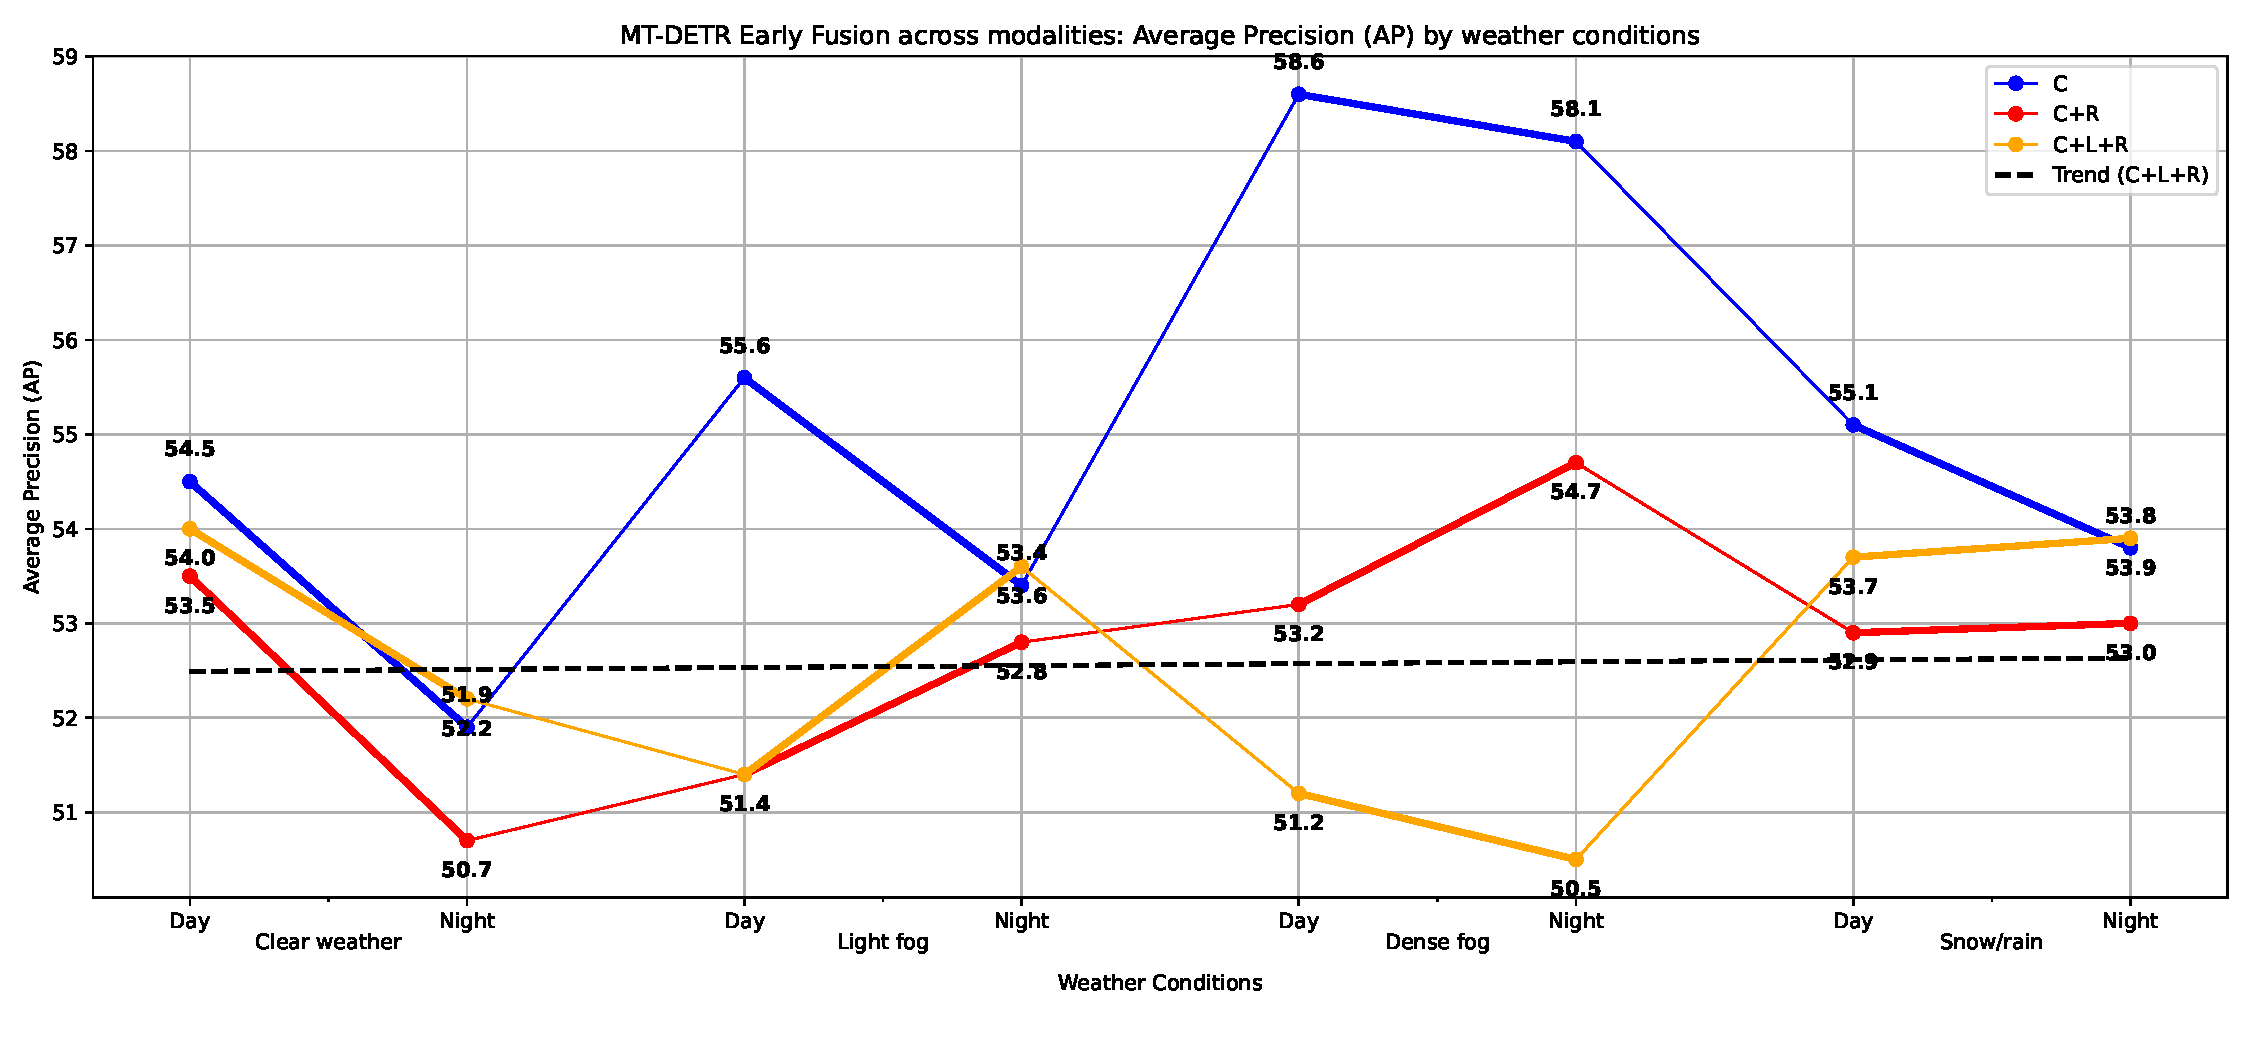
\includegraphics[width=1.0\textwidth]{images/results/mtdetr/early/ap.pdf}
            \caption{Performance of the MT-DETR Early Fusion model in terms of AP across sensor modalities under different weather conditions. Note: C data point values are shown above the line and rest are below the line.}
            \label{fig:mtdetr_early_ap}
        \end{figure}

        \begin{figure}[]
            \centering
            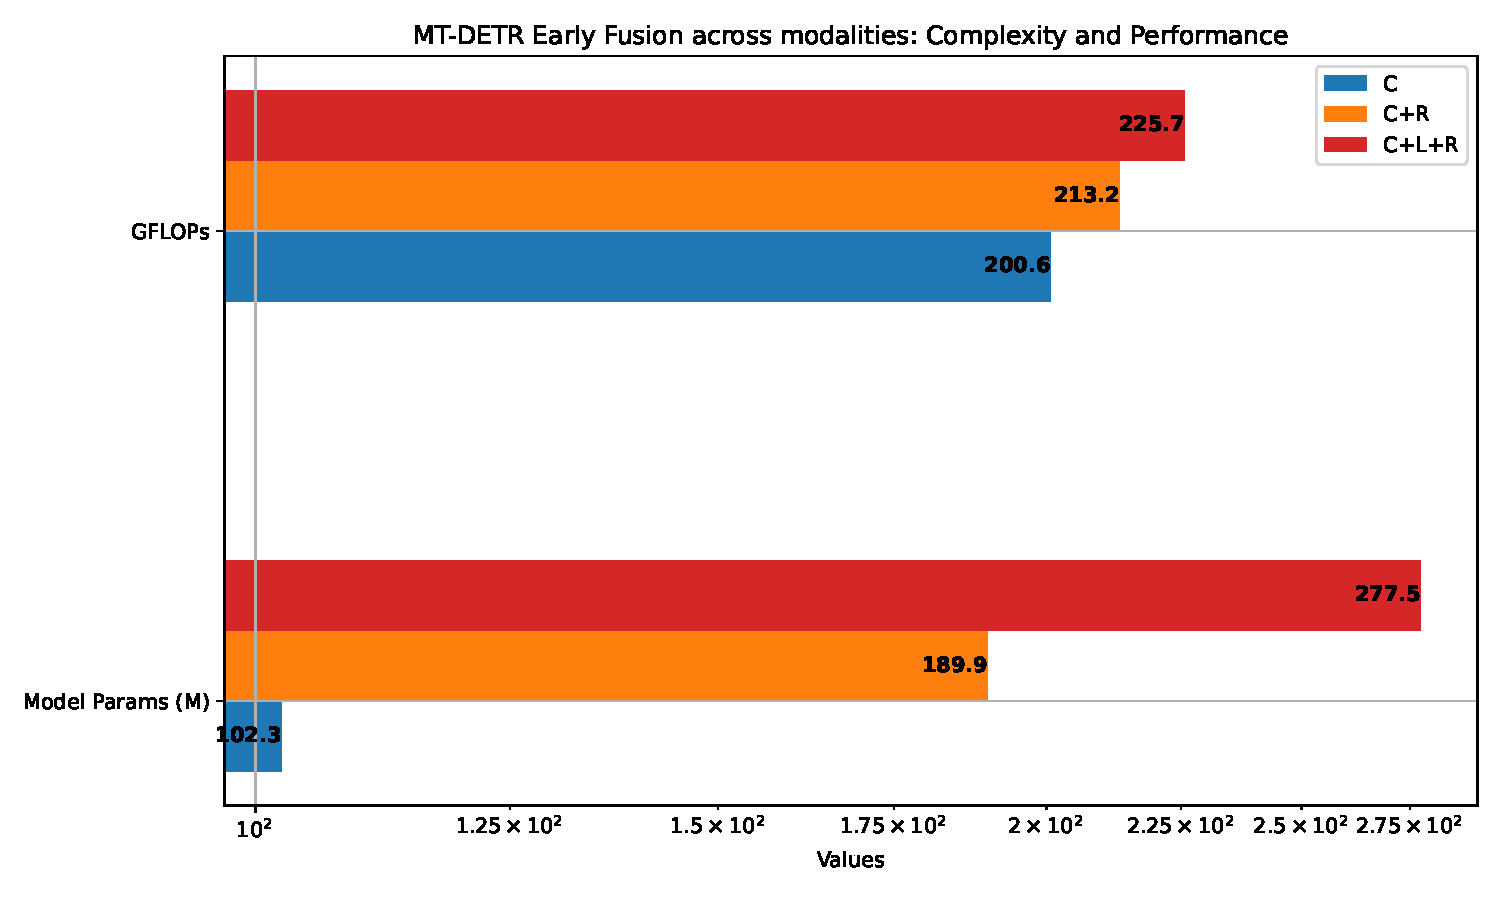
\includegraphics[width=0.8\textwidth]{images/results/mtdetr/early/model_complexity.pdf}
            \caption{MT-DETR Early Fusion model's complexity, displayed through model parameters (in M), and GFLOPs across different sensor modalities.}
            \label{fig:mtdetr_early_model_complexity}
        \end{figure}

    \FloatBarrier
    \subsubsection{Middle Fusion: C vs. C+R vs. C+L+R}

    In the case of the Middle Fusion or Feature Fusion model, the combination of Camera, LiDAR, and Radar (C+L+R) yields the most effective results. This fusion technique operates by selecting the optimal features from the input modalities. These selections occur after the data has undergone the initial stages of feature extraction, ensuring that only the most relevant and reliable features are utilized for further processing.

    \begin{figure}[h!]
        \centering
        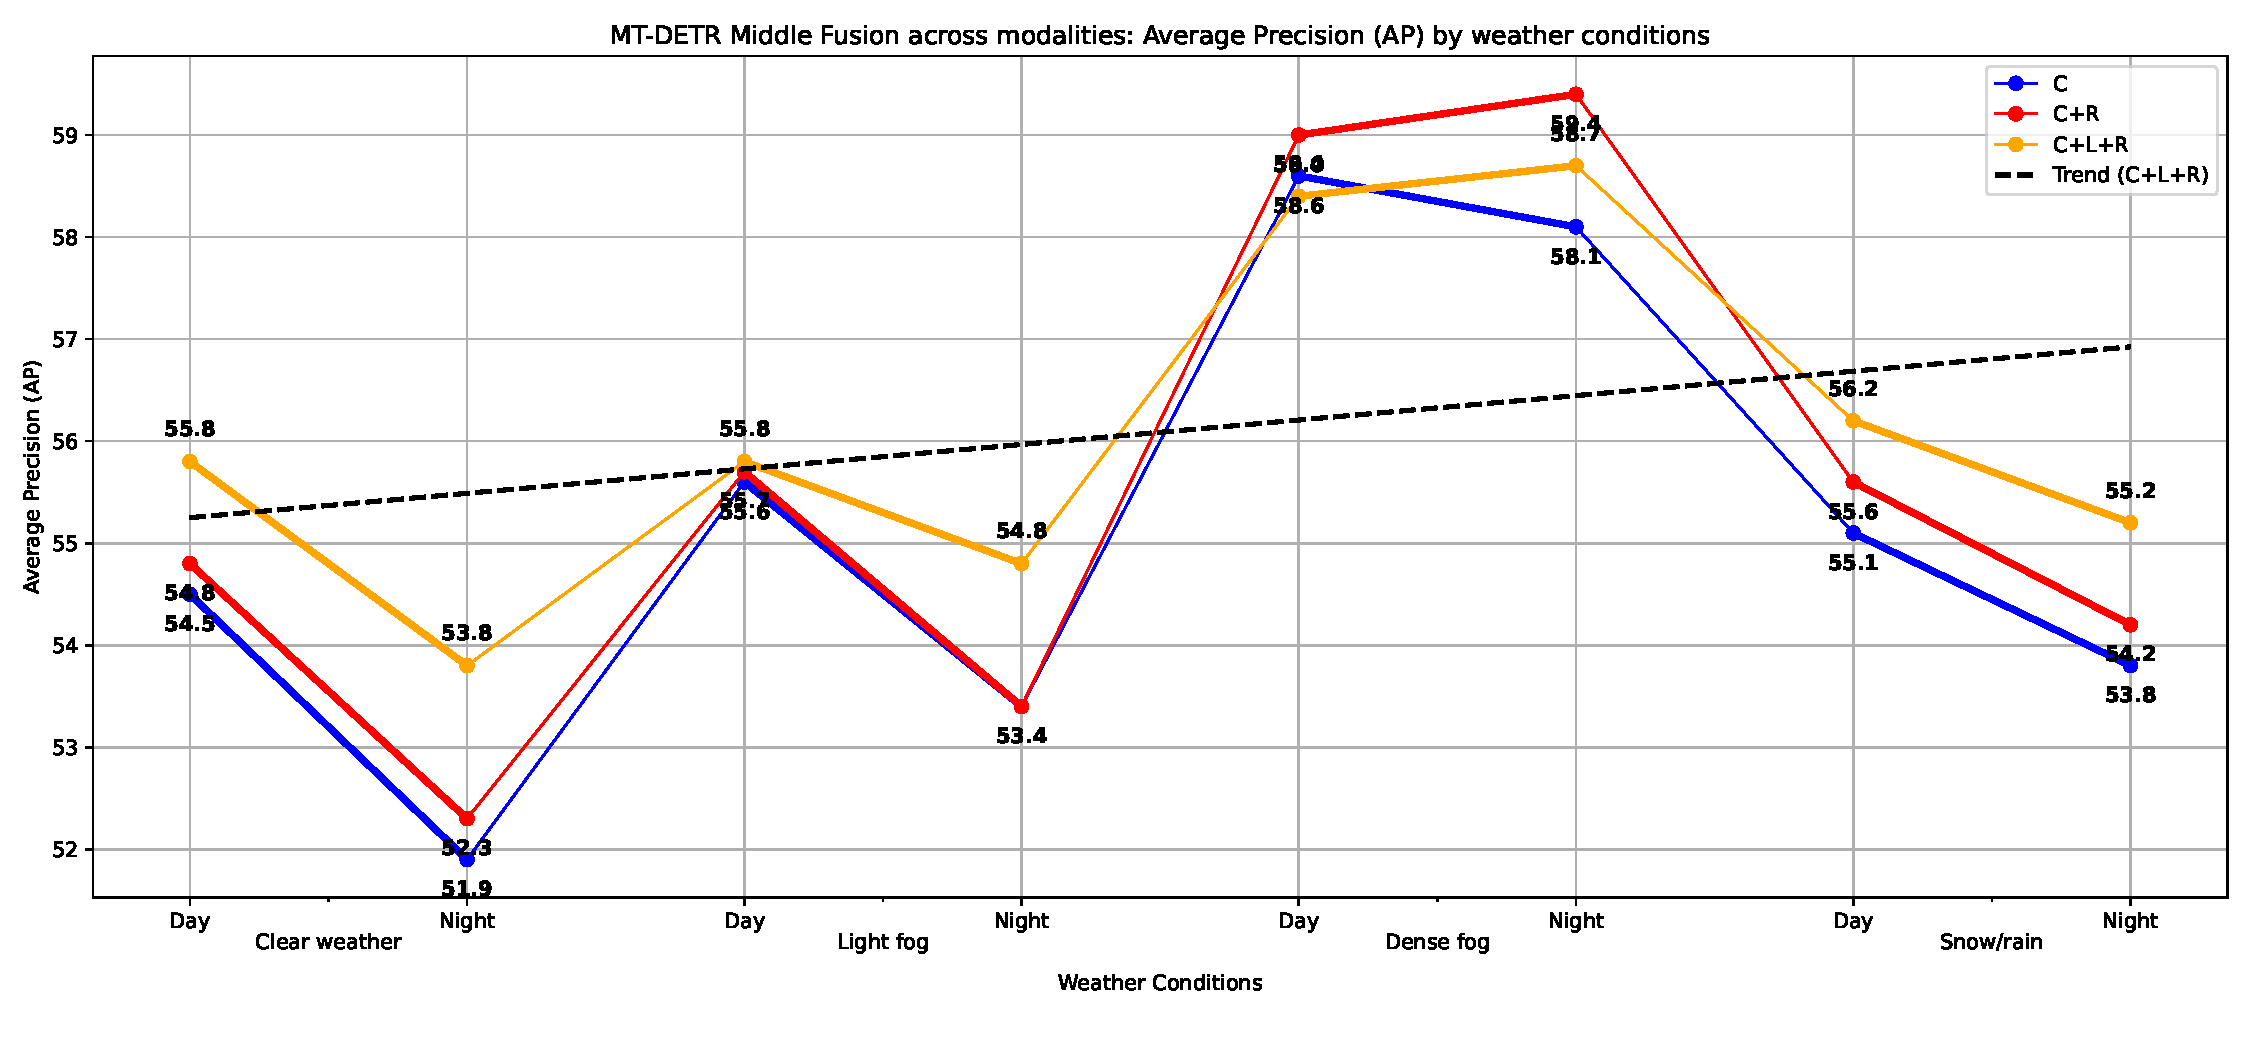
\includegraphics[width=1.0\textwidth]{images/results/mtdetr/middle/ap.pdf}
        \caption{Performance of the MT-DETR Middle Fusion model in terms of AP across sensor modalities under different weather conditions. Note: C+L+R data point values are shown above the line and rest are below the line.}
        \label{fig:mtdetr_middle_ap}
    \end{figure}

    \begin{figure}[h!]
        \centering
        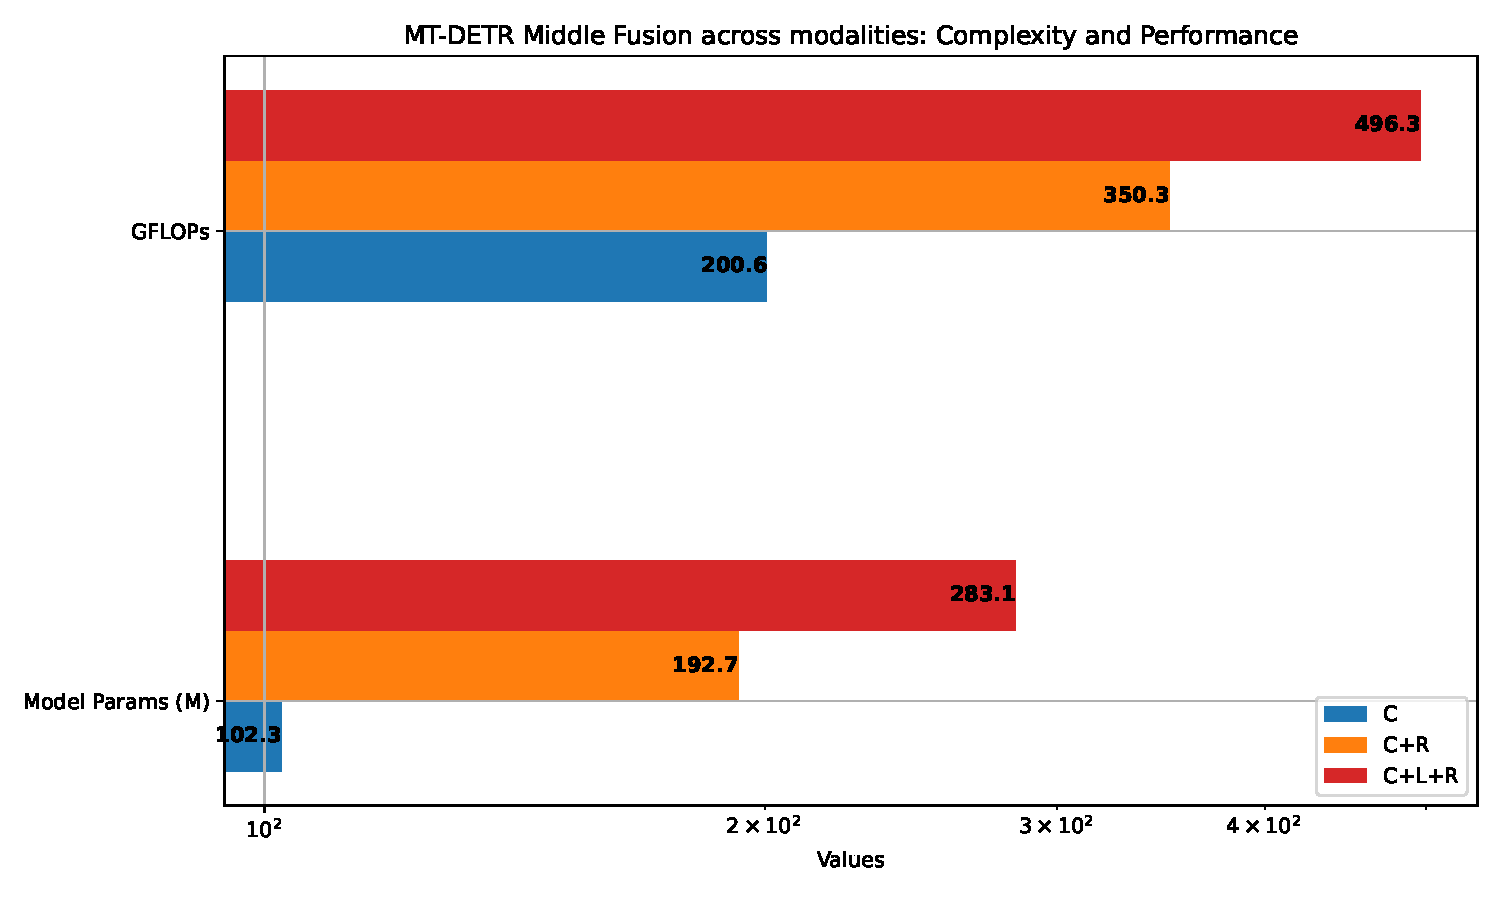
\includegraphics[width=0.8\textwidth]{images/results/mtdetr/middle/model_complexity.pdf}
        \caption{MT-DETR Middle Fusion model's complexity, displayed through model parameters (in M), and GFLOPs across different sensor modalities.}
        \label{fig:mtdetr_middle_model_complexity}
    \end{figure}

    \FloatBarrier
    \subsubsection{Tightly-Coupled Fusion: C vs. C+R vs. C+L+R}

    In this experiment, it is crucial to highlight that the Camera and Radar (C+R) modality significantly outperforms other configurations, particularly in dense fog weather conditions. This indicates that the MT-DETR Tightly-Coupled Fusion architecture effectively extracts the most relevant features from the sensor least affected by adverse conditions, in this case, the radar. This selective extraction is key to achieving the final, robust results.

    \begin{figure}[h!]
        \centering
        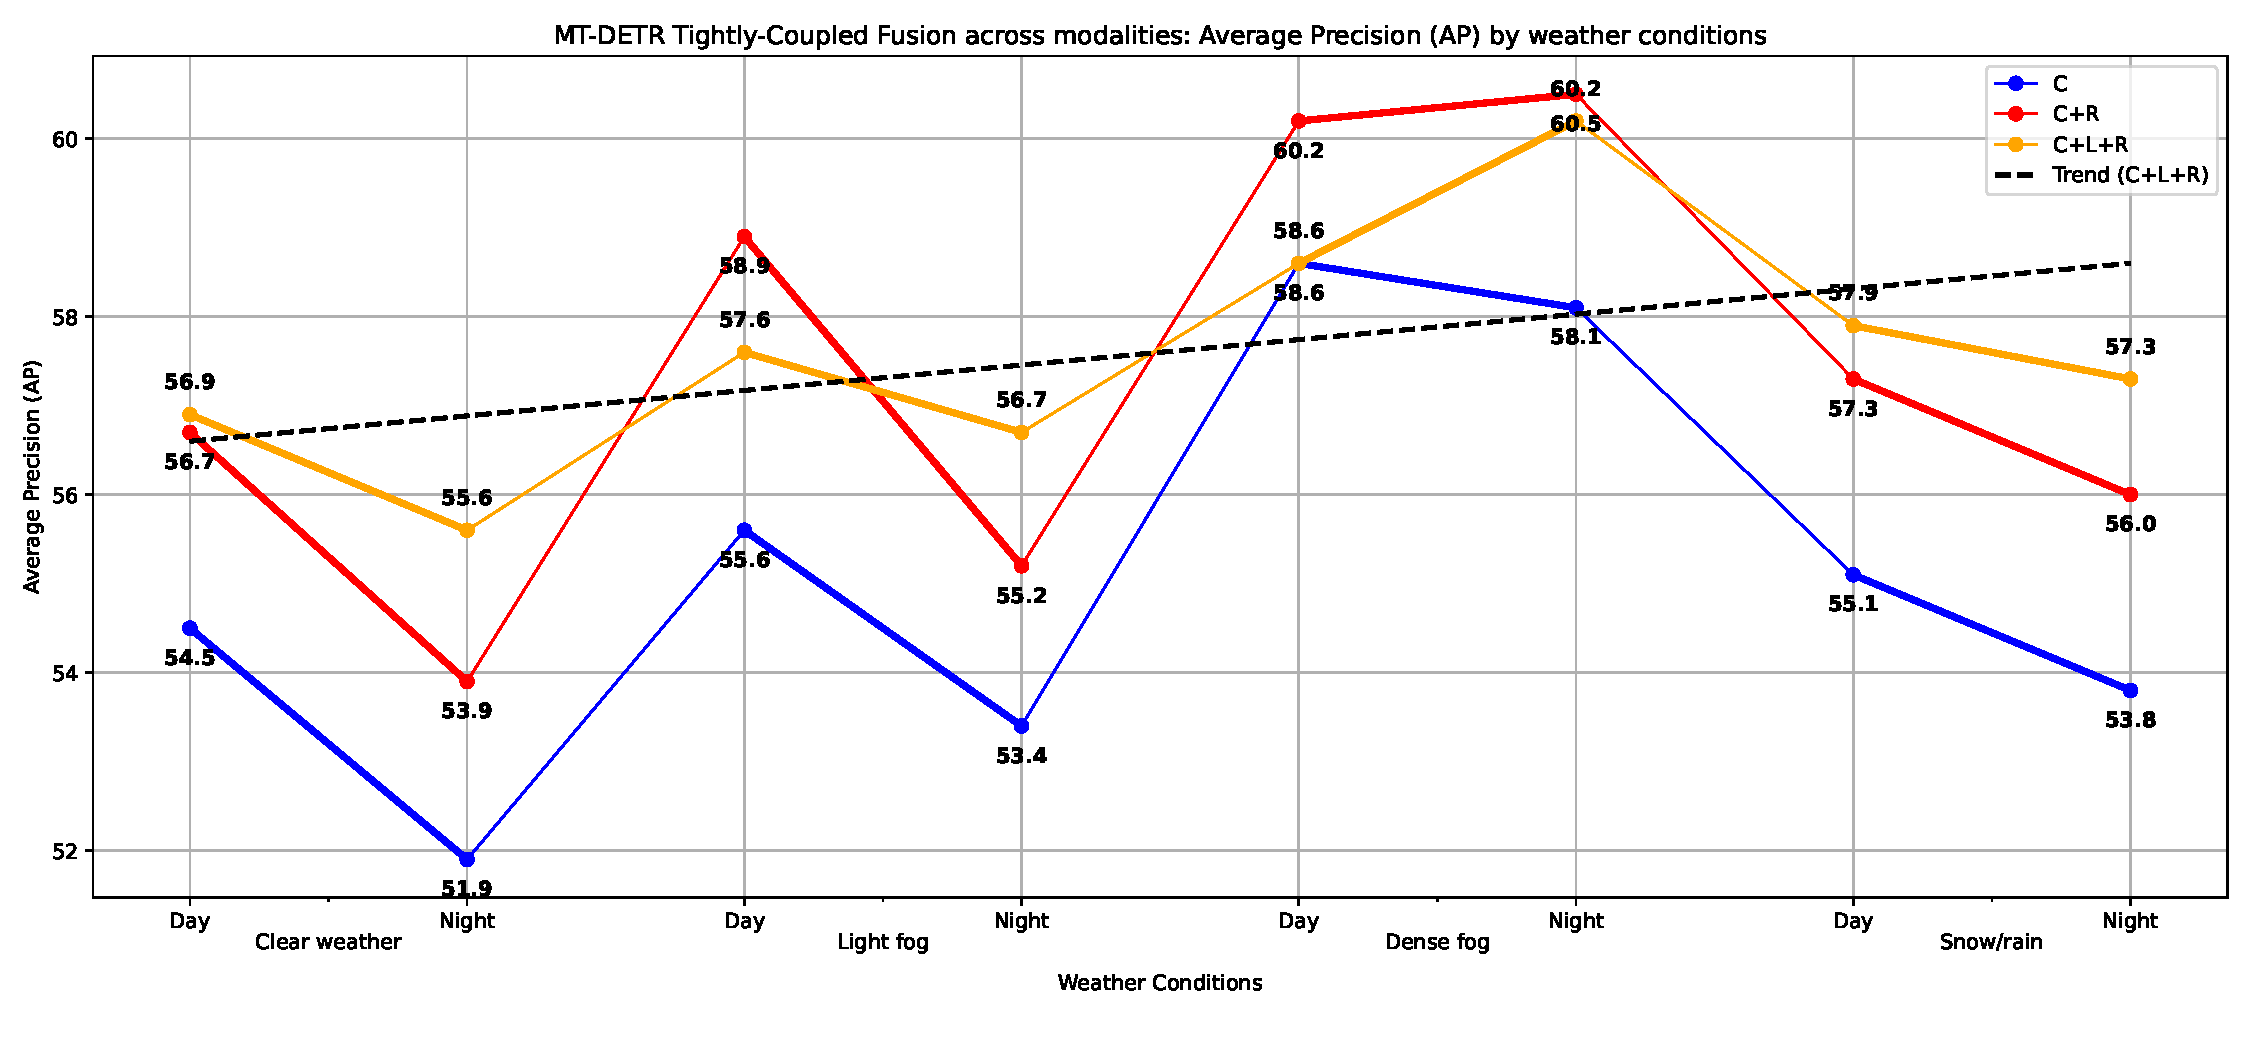
\includegraphics[width=1.0\textwidth]{images/results/mtdetr/tight/ap.pdf}
        \caption{Performance of the MT-DETR Tightly-Coupled Fusion model in terms of AP across sensor modalities under different weather conditions. Note: C+L+R data point values are shown above the line and rest are below the line.}
        \label{fig:mtdetr_tight_ap}
    \end{figure}

    \begin{figure}[h!]
        \centering
        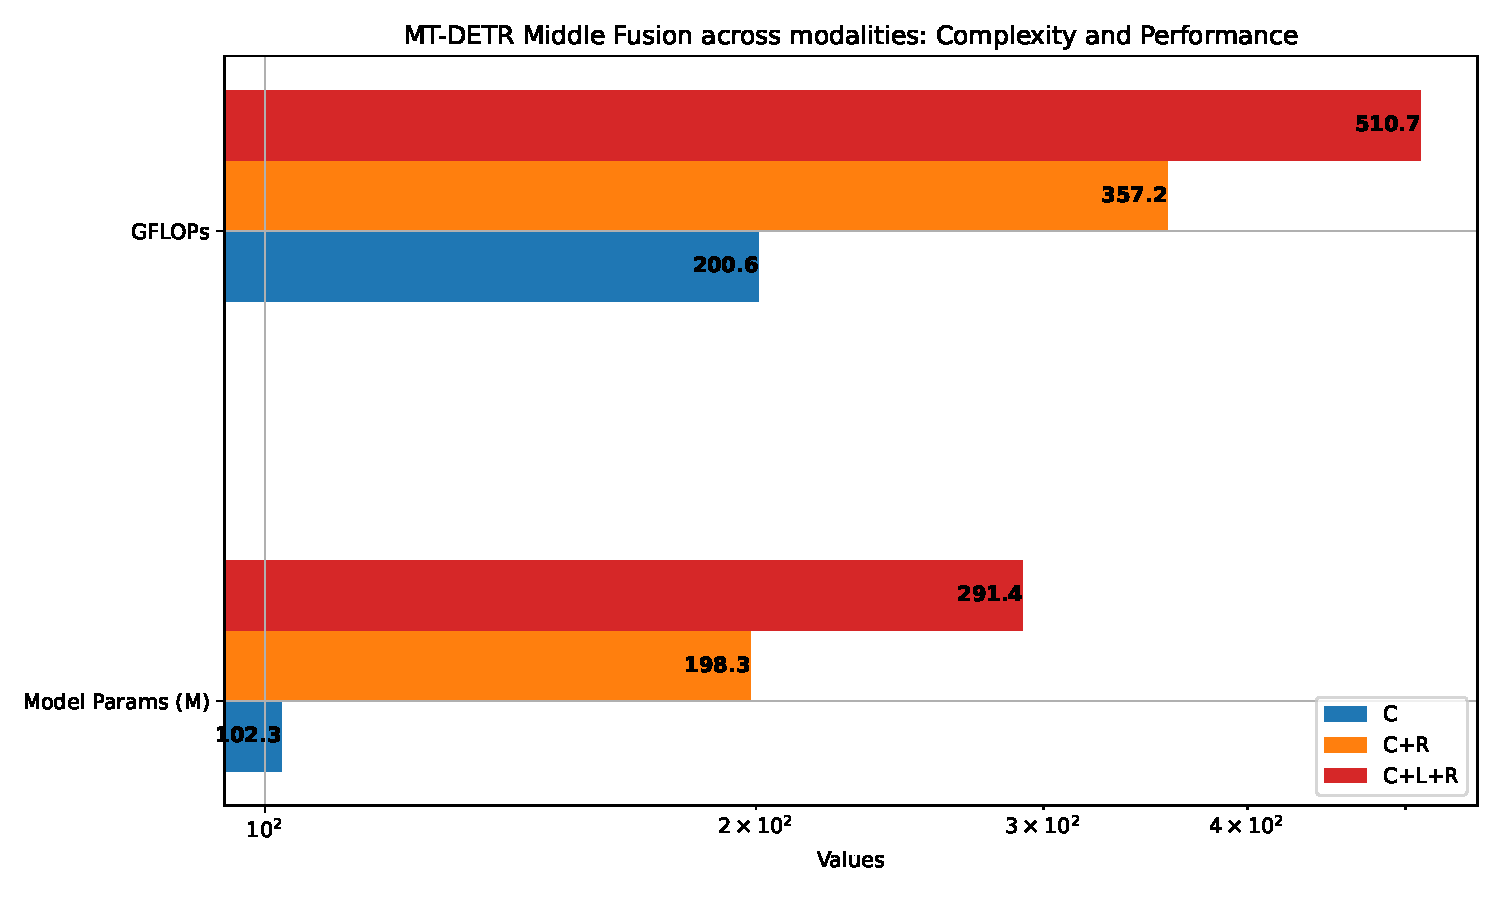
\includegraphics[width=0.8\textwidth]{images/results/mtdetr/tight/model_complexity.pdf}
        \caption{MT-DETR Tightly-Coupled Fusion model's complexity, displayed through model parameters (in M), and GFLOPs across different sensor modalities.}
        \label{fig:mtdetr_tight_model_complexity}
    \end{figure}


    

    \FloatBarrier
    \subsubsection{Early vs. Middle vs. Tightly-Coupled Fusion: C+R}

    The subsequent two experiments involve a comparative analysis of Early, Middle, and Tightly-Coupled Fusion models using various sensor modalities. In both comparative studies, the Tightly-Coupled Fusion model consistently outperforms the other fusion architectures. This consistent superiority underscores the significance of integrating features at multiple stages from diverse input modalities, demonstrating the effectiveness of this approach in enhancing model performance. 

    \begin{figure}[h!]
        \centering
        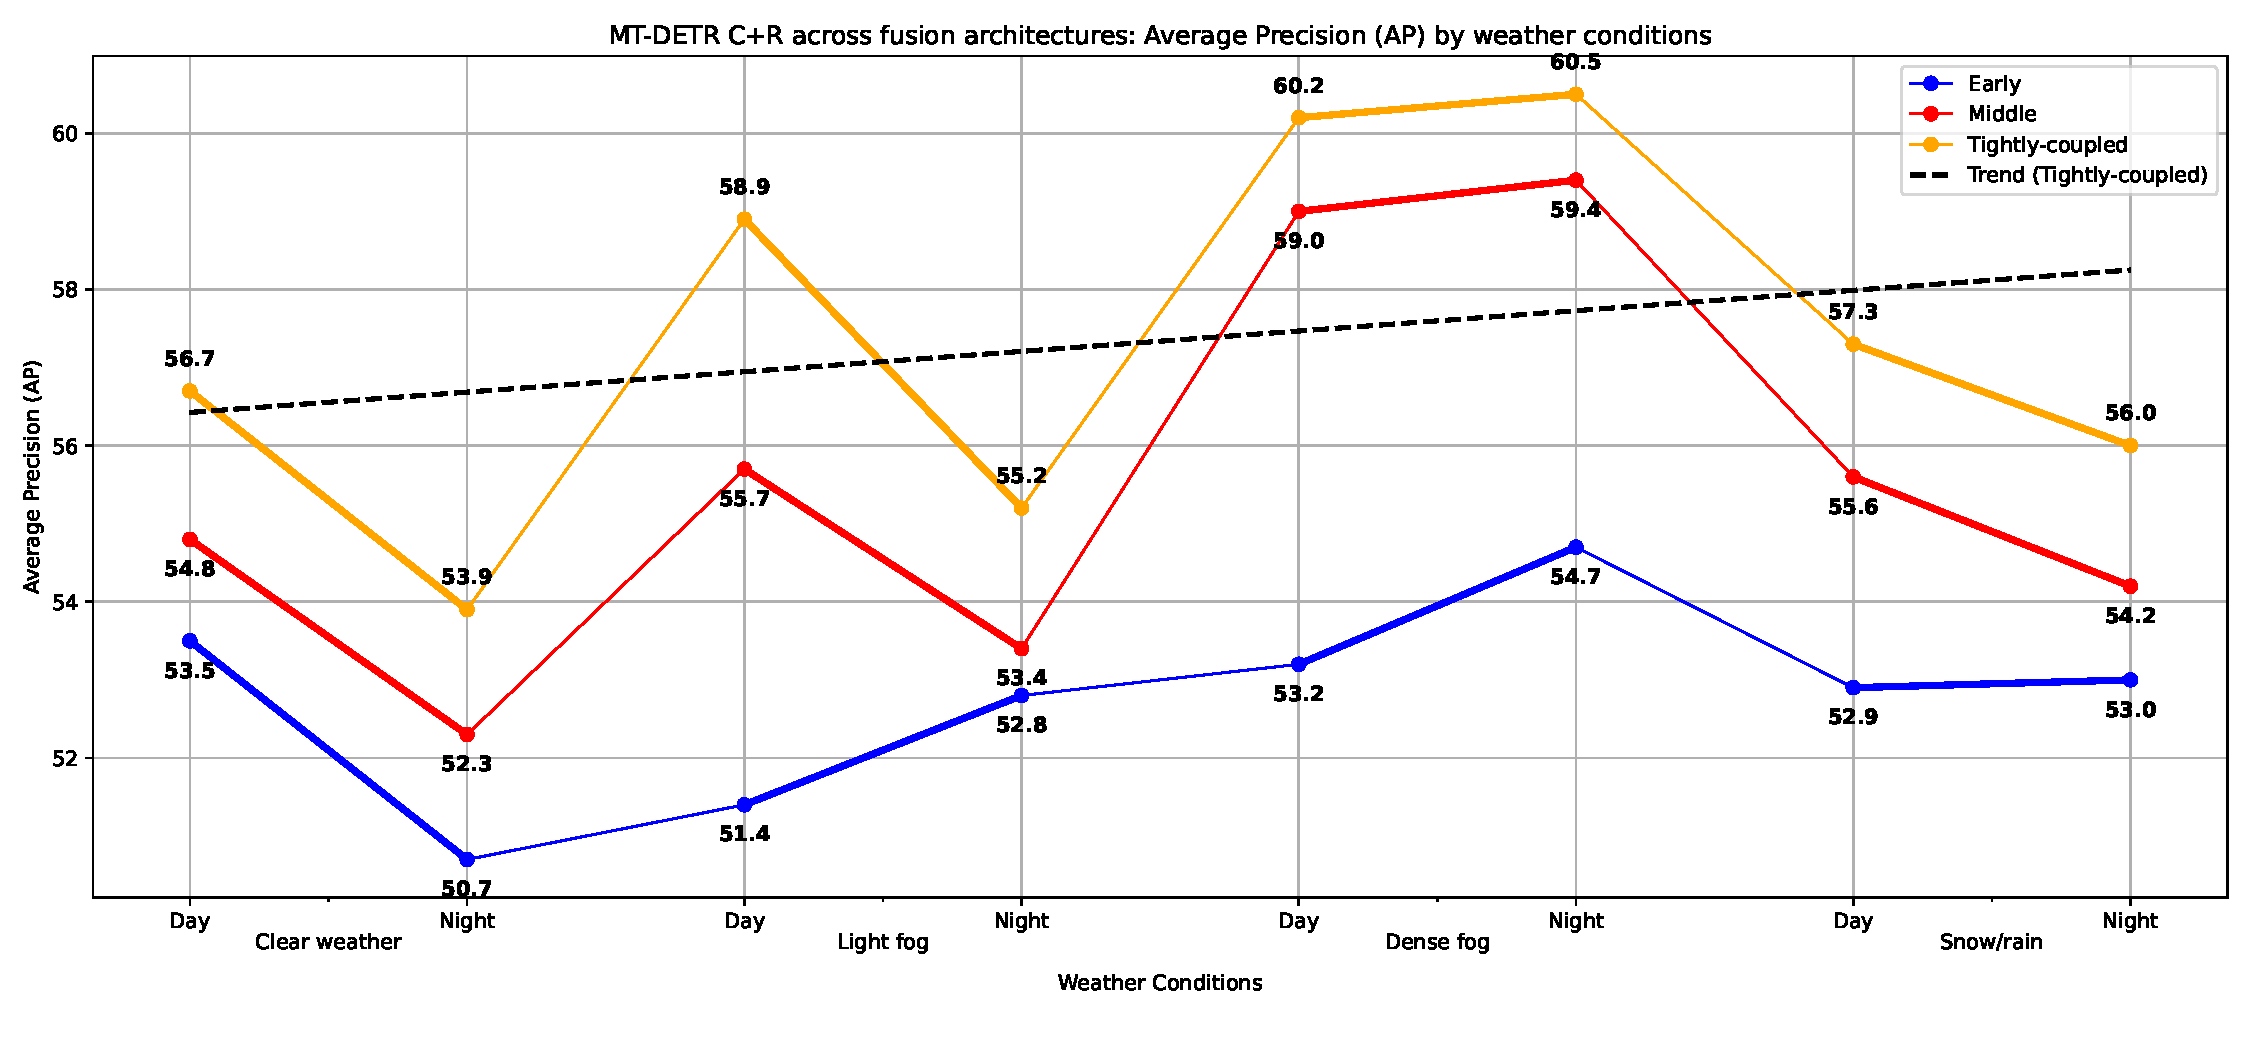
\includegraphics[width=1.0\textwidth]{images/results/mtdetr/EMT_CR/ap.pdf}
        \caption{Performance of the MT-DETR across the Early, Middle, and Tightly-Coupled Fusion model with C+R in terms of AP across sensor modalities under different weather conditions. Note: Tightly-Coupled data point values are shown above the line and rest are below the line.}
        \label{fig:mtdetr_emt_cr_ap}
    \end{figure}

    \begin{figure}[h!]
        \centering
        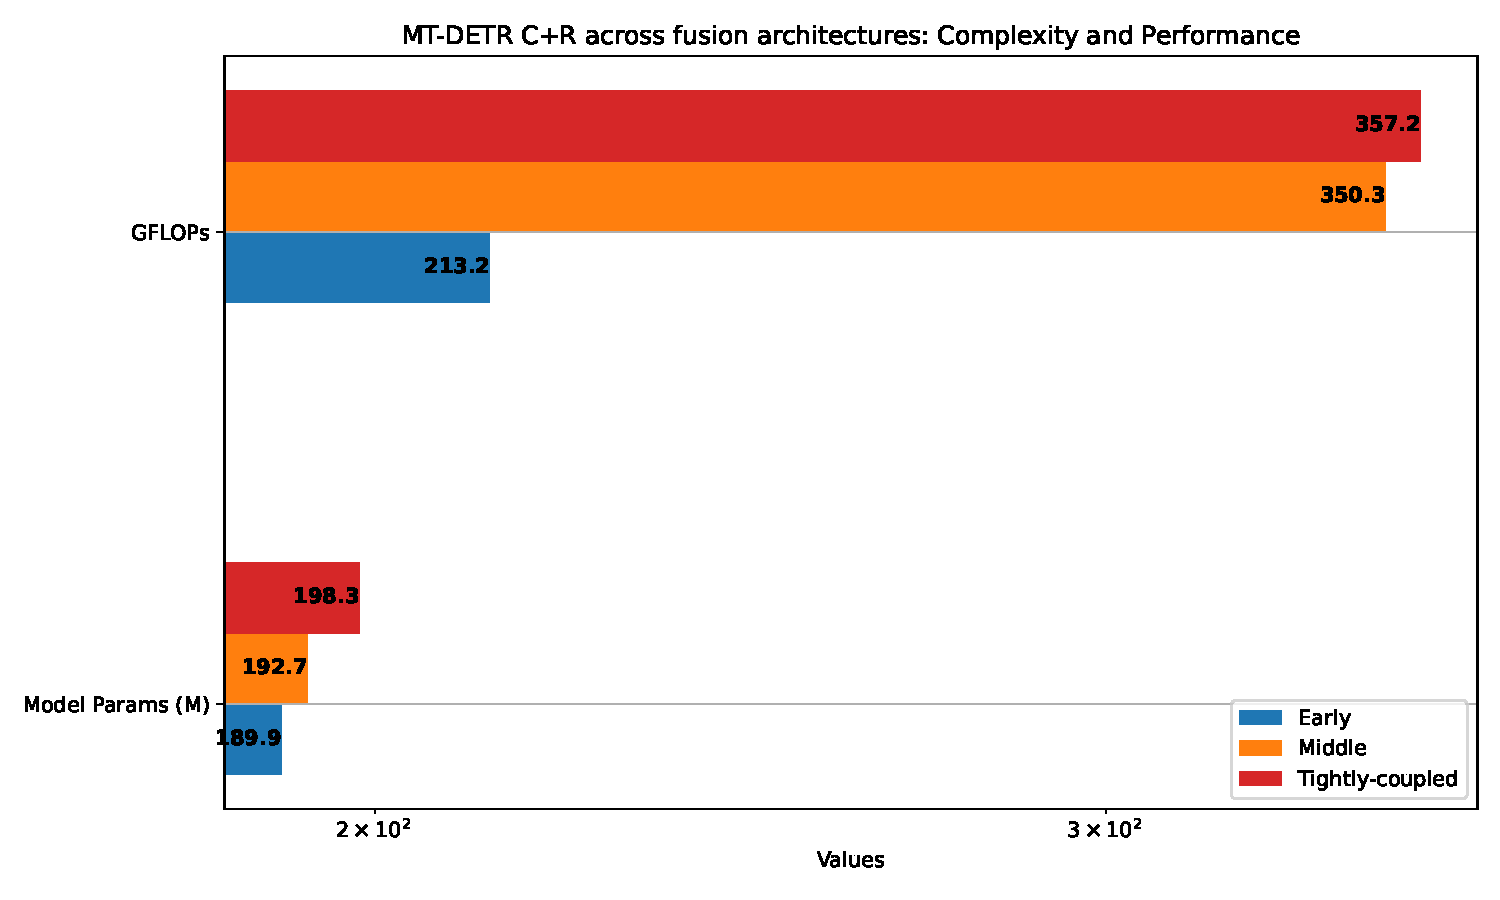
\includegraphics[width=0.8\textwidth]{images/results/mtdetr/EMT_CR/model_complexity.pdf}
        \caption{MT-DETR model's complexity across the Early, Middle, and Tightly-Coupled Fusion with C+R, displayed through model parameters (in M), and GFLOPs.}
        \label{fig:mtdetr_emt_cr_model_complexity}
    \end{figure}

    \FloatBarrier
    \subsubsection{Early vs. Middle vs. Tightly-Coupled Fusion: C+L+R}

    \begin{figure}[h!]
        \centering
        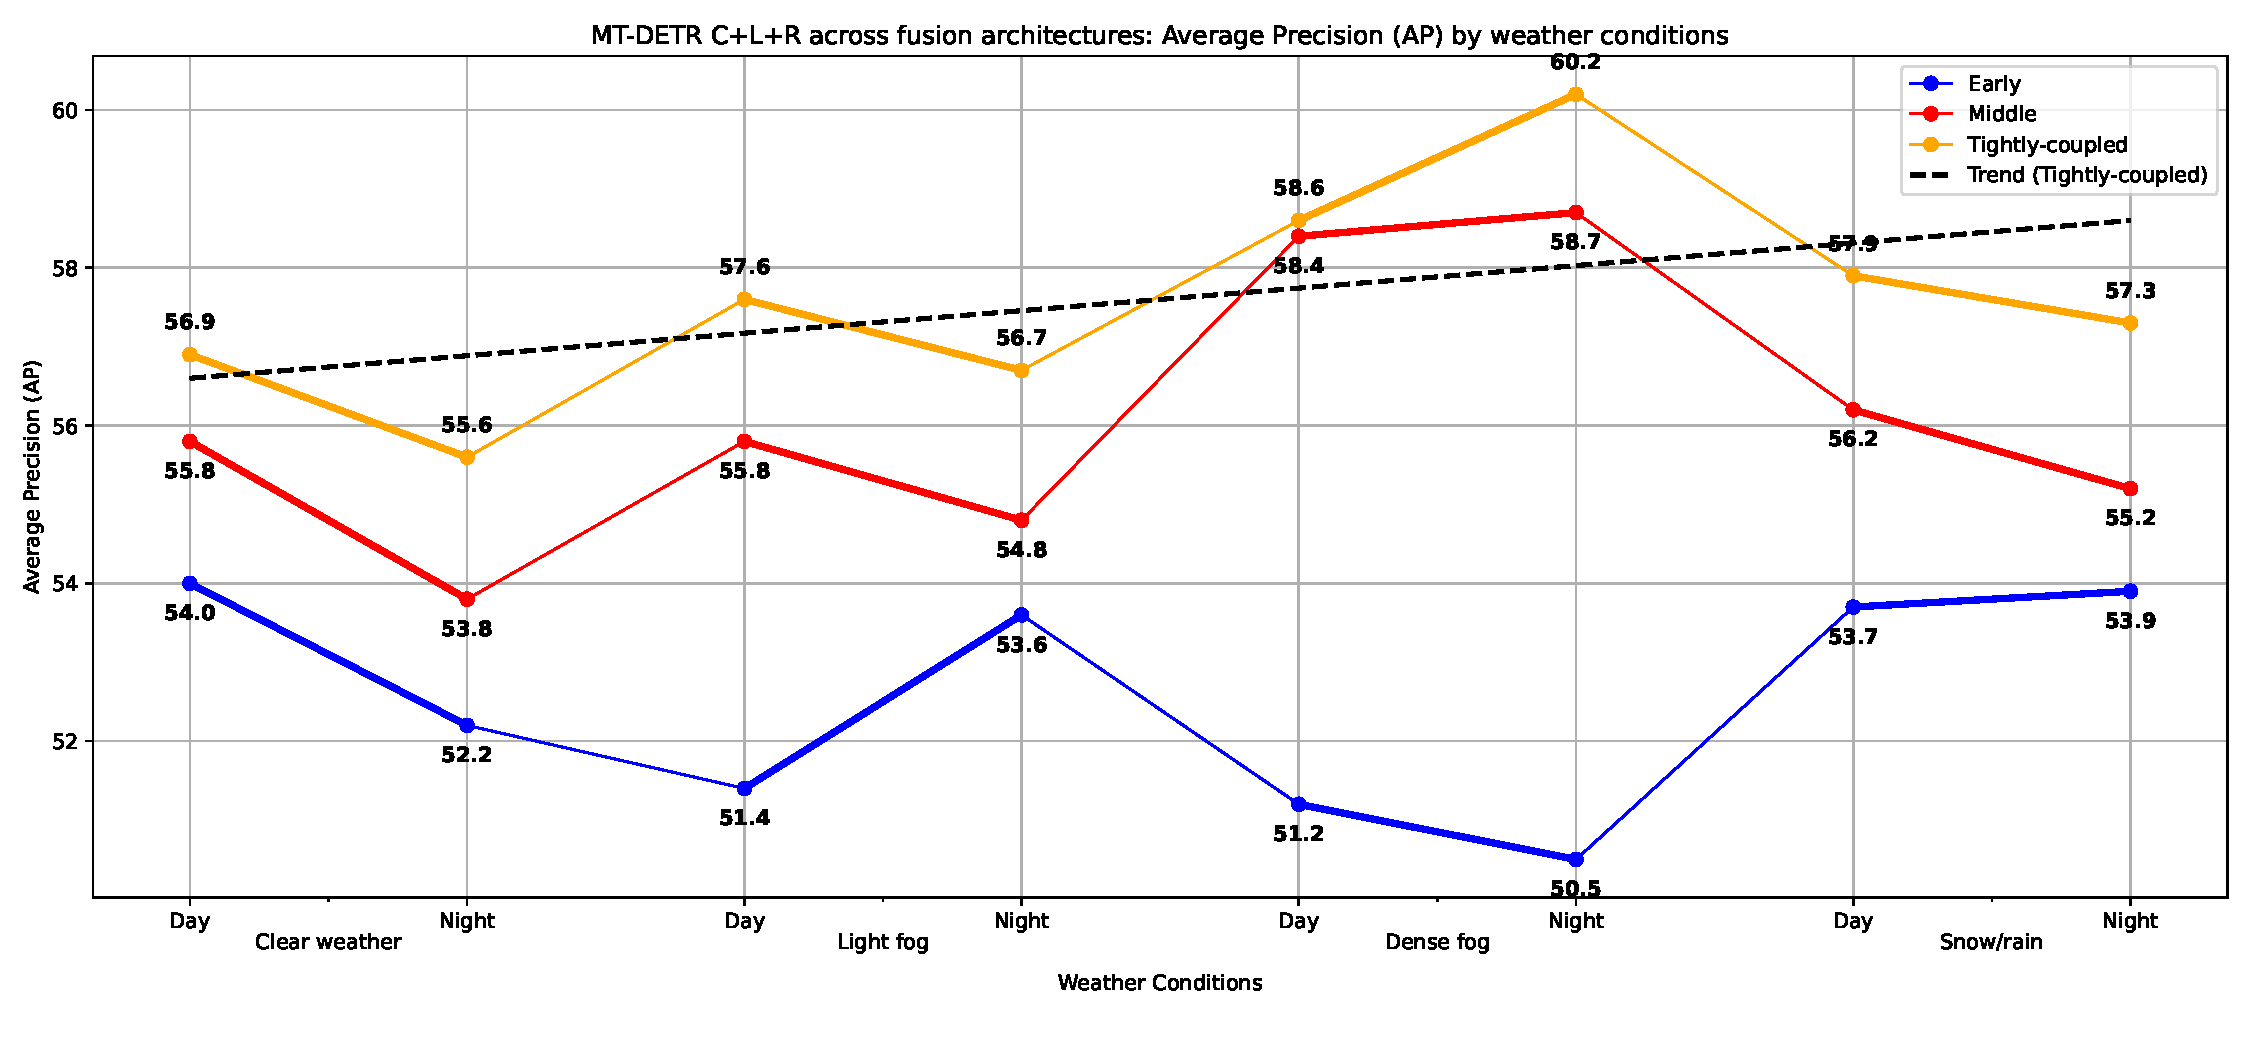
\includegraphics[width=1.0\textwidth]{images/results/mtdetr/EMT_CLR/ap.pdf}
        \caption{Performance of the MT-DETR across the Early, Middle, and Tightly-Coupled Fusion model with C+L+R in terms of AP across sensor modalities under different weather conditions. Note: Tightly-Coupled data point values are shown above the line and rest are below the line.}
        \label{fig:mtdetr_emt_crl_ap}
    \end{figure}

    \begin{figure}[h!]
        \centering
        \includegraphics[width=0.8\textwidth]{images/results/mtdetr/EMT_CLR/model_complexity.pdf}
        \caption{MT-DETR model's complexity across the Early, Middle, and Tightly-Coupled Fusion with C+L+R, displayed through model parameters (in M), and GFLOPs.}
        \label{fig:mtdetr_emt_crl_model_complexity}
    \end{figure}

    \FloatBarrier
    \subsubsection{Tightly-Coupled Fusion (with Time): C+R vs. C+L+R vs. C+L+R+T}

    \begin{figure}[h!]
        \centering
        \includegraphics[width=1.0\textwidth]{images/results/mtdetr/T_CLRT/ap.pdf}
        \caption{Performance of the MT-DETR Tightly-Coupled Fusion with additional Time input in terms of AP across sensor modalities under different weather conditions. Note: C+L+R+T data point values are shown above the line and rest are below the line.}
        \label{fig:mtdetr_t_clrt_ap}
    \end{figure}

    \begin{figure}[h!]
        \centering
        \includegraphics[width=0.8\textwidth]{images/results/mtdetr/T_CLRT/model_complexity.pdf}
        \caption{MT-DETR Tightly-Coupled Fusion model's complexity across modalities, displayed through model parameters (in M), and GFLOPs.}
        \label{fig:mtdetr_t_clrt_model_complexity}
    \end{figure}

    \paragraph*{Qualitative Analysis: Comparison across Fusion Architectures}

    Here, we present the detection results of MT-DETR across different fusion architectures. Figure \ref{fig:mtdetr_on_dense} below illustrates the detection results comparing the Middle and Tightly-Coupled Fusion architectures with the Camera, LiDAR and Radar sensor fusion. From the above quantitative analysis, it is clear that Middle Fusion outperforms Early Fusion, hence for qualitative analysis, we only consider the Middle Fusion and Tightly-Coupled Fusion.

    The qualitative analysis reveals that Middle Fusion is generally effective in adverse weather conditions. However, it encounters challenges in certain extreme cases, such as detecting small, distant objects, as illustrated in rows 1, 4, and 5 of Figure \ref{fig:mtdetr_on_dense}. A notable instance of its limitation is presented in row 2, where Middle Fusion incorrectly identifies a car's reflection in a mirror. This error likely stems from its inability to robustly integrate data from the depth sensor with the camera information. Additionally, row 3 highlights another issue where the system successfully detects an object but erroneously categorizes a pedestrian as a vehicle.

    Notice that in the last two samples, despite the absence of ground truth annotations, the Tightly-Coupled Fusion model effectively identifies the objects. This observation is particularly significant given that all models were trained solely in clear weather conditions and had no prior exposure to such extreme and challenging weather scenarios in their training phase. Nevertheless, the models demonstrate robust performance, a testament to the MT-DETR model architecture. This architecture excels in extracting maximal information from all available sensors and integrating it at various stages. This capability highlights the model's proficiency in adapting to and overcoming the limitations posed by unforeseen and adverse environmental conditions.

    
    \begin{figure}[h!]
        \centering
        % Row 1
        \includegraphics[width=0.3\textwidth]{images/results/mtdetr/samples/day_snow/2018-02-04_12-37-52_00100_gt.png}
        \includegraphics[width=0.3\textwidth]{images/results/mtdetr/samples/day_snow/2018-02-04_12-37-52_00100_m_clr.png}
        \includegraphics[width=0.3\textwidth]{images/results/mtdetr/samples/day_snow/2018-02-04_12-37-52_00100_t_clr.png}
      
        % Row 2
        \includegraphics[width=0.3\textwidth]{images/results/mtdetr/samples/day_snow_2/2018-02-04_11-29-58_00200_gt.png}
        \includegraphics[width=0.3\textwidth]{images/results/mtdetr/samples/day_snow_2/2018-02-04_11-29-58_00200_mid_clr.png}
        \includegraphics[width=0.3\textwidth]{images/results/mtdetr/samples/day_snow_2/2018-02-04_11-29-58_00200_tight_clr.png}
      
        % % Row 3
        \includegraphics[width=0.3\textwidth]{images/results/mtdetr/samples/night_dense_fog/2018-02-07_18-26-13_00240_gt.png}
        \includegraphics[width=0.3\textwidth]{images/results/mtdetr/samples/night_dense_fog/2018-02-07_18-26-13_00240_m_clr.png}
        \includegraphics[width=0.3\textwidth]{images/results/mtdetr/samples/night_dense_fog/2018-02-07_18-26-13_00240_t_clr.png}
      
        % % Row 4
        \includegraphics[width=0.3\textwidth]{images/results/mtdetr/samples/night_snow/2018-02-08_17-45-07_00270_gt.png}
        \includegraphics[width=0.3\textwidth]{images/results/mtdetr/samples/night_snow/2018-02-08_17-45-07_00270_m_clr.png}
        \includegraphics[width=0.3\textwidth]{images/results/mtdetr/samples/night_snow/2018-02-08_17-45-07_00270_t_clr.png}
      
        % % Row 5
        \includegraphics[width=0.3\textwidth]{images/results/mtdetr/samples/snow_1/2018-02-12_09-32-09_00510_gt.png}
        \includegraphics[width=0.3\textwidth]{images/results/mtdetr/samples/snow_1/2018-02-12_09-32-09_00510_m_clr.png}
        \includegraphics[width=0.3\textwidth]{images/results/mtdetr/samples/snow_1/2018-02-12_09-32-09_00510_t_clr.png}

        % % Row 6
        \includegraphics[width=0.3\textwidth]{images/results/mtdetr/samples/snow_2/2018-02-12_18-05-56_00060_gt.png}
        \includegraphics[width=0.3\textwidth]{images/results/mtdetr/samples/snow_2/2018-02-12_18-05-56_00060_m_clr.png}
        \includegraphics[width=0.3\textwidth]{images/results/mtdetr/samples/snow_2/2018-02-12_18-05-56_00060_t_clr.png}

        % % Row 7
        \includegraphics[width=0.3\textwidth]{images/results/mtdetr/samples/snow_3/2018-02-12_10-07-06_00200_gt.png}
        \includegraphics[width=0.3\textwidth]{images/results/mtdetr/samples/snow_3/2018-02-12_10-07-06_00200_m_clr.png}
        \includegraphics[width=0.3\textwidth]{images/results/mtdetr/samples/snow_3/2018-02-12_10-07-06_00200_t_clr.png}
        % % Row 8
        \includegraphics[width=0.3\textwidth]{images/results/mtdetr/samples/snow_4/2018-02-12_11-00-35_00450_gt.png}
        \includegraphics[width=0.3\textwidth]{images/results/mtdetr/samples/snow_4/2018-02-12_11-00-35_00450_m_clr.png}
        \includegraphics[width=0.3\textwidth]{images/results/mtdetr/samples/snow_4/2018-02-12_11-00-35_00450_t_clr.png}
      
        \caption{A few samples to showcase the detection results of MT-DETR. Where the 1st column is ground truth, 2nd is Middle Fusion, and 3rd is Tightly-Coupled Fusion, both are using the same C+L+R (Rows show the extremely challenging weather conditions). Best viewed in zoomed-in view.}
        \label{fig:mtdetr_on_dense}
      \end{figure}


% ####################################################
% #####################################################
% ###################################################


    \subsection{MT-DETR vs. HRFuser: Tightly-Coupled Fusion}

    This section shows the comparison between the MT-DETR and HRFuser Tightly-Coupled Fusion models. Both are evaluated on the same test set from the DENSE dataset. Both models are compared across various sensor modalities, including C+R, C+L, C+L+R, and C+L+R+T.

    It is important to note that for a fair comparison of floating-point operations (FLOPs) between HRFuser and MT-DETR, we ensured that both models used the same input dimensions. This is crucial since FLOPs are highly dependent on the size of the input dimension. 

    \FloatBarrier
    \subsubsection{Compared on C+R}

    \begin{figure}[h!]
        \centering
        \includegraphics[width=1.0\textwidth]{images/results/hrfuser_vs_mtdetr/cr/ap.pdf}
        \caption{Performance of the MT-DETR vs. HRFuser with Tightly-Coupled Fusion on C+R in terms of AP under different weather conditions. Note: MT-DETR data point values are shown above the line.}
        \label{fig:hrfuser_vs_mtdetr_cr_ap}
    \end{figure}

    \begin{figure}[h!]
        \centering
        \includegraphics[width=0.8\textwidth]{images/results/hrfuser_vs_mtdetr/cr/model_complexity.pdf}
        \caption{MT-DETR vs. HRFuser: Tightly-Coupled Fusion model's complexity on C+R displayed through model parameters (in M), and GFLOPs.}
        \label{fig:hrfuser_vs_mtdetr_cr_model_complexity}
    \end{figure}

    \FloatBarrier
    \subsubsection{Compared on C+L}

    \begin{figure}[h!]
        \centering
        \includegraphics[width=1.0\textwidth]{images/results/hrfuser_vs_mtdetr/cl/ap.pdf}
        \caption{Performance of the MT-DETR vs. HRFuser with Tightly-Coupled Fusion on C+L in terms of AP under different weather conditions. Note: MT-DETR data point values are shown above the line.}
        \label{fig:hrfuser_vs_mtdetr_cl_ap}
    \end{figure}
    \begin{figure}[h!]
        \centering
        \includegraphics[width=0.8\textwidth]{images/results/hrfuser_vs_mtdetr/cl/model_complexity.pdf}
        \caption{MT-DETR vs. HRFuser: Tightly-Coupled Fusion model's complexity on C+L displayed through model parameters (in M), and GFLOPs.}
        \label{fig:hrfuser_vs_mtdetr_cl_model_complexity}
    \end{figure}

    \FloatBarrier
    \subsubsection{Compared on C+L+R}

    \begin{figure}[h!]
        \centering
        \includegraphics[width=1.0\textwidth]{images/results/hrfuser_vs_mtdetr/clr/ap.pdf}
        \caption{Performance of the MT-DETR vs. HRFuser with Tightly-Coupled Fusion on C+L+R in terms of AP under different weather conditions. Note: MT-DETR data point values are shown above the line.}
        \label{fig:hrfuser_vs_mtdetr_clr_ap}
    \end{figure}

    \begin{figure}[h!]
        \centering
        \includegraphics[width=0.8\textwidth]{images/results/hrfuser_vs_mtdetr/clr/model_complexity.pdf}
        \caption{MT-DETR vs. HRFuser: Tightly-Coupled Fusion model's complexity on C+L+R displayed through model parameters (in M), and GFLOPs.}
        \label{fig:hrfuser_vs_mtdetr_clr_model_complexity}
    \end{figure}
    \FloatBarrier
    \subsubsection{Compared on C+L+R+T (MT-DETR) vs. C+L+R+G (HRFuser)}

    \begin{figure}[h!]
        \centering
        \includegraphics[width=1.0\textwidth]{images/results/hrfuser_vs_mtdetr/clr_g_t/ap.pdf}
        \caption{Performance of the MT-DETR vs. HRFuser with Tightly-Coupled Fusion on C+L+R + additional input(Time vs. Gated) in terms of AP under different weather conditions. Note: MT-DETR data point values are shown above the line.}
        \label{fig:hrfuser_vs_mtdetr_clr_g_t_ap}
    \end{figure}

    \begin{figure}[h!]
        \centering
        \includegraphics[width=0.8\textwidth]{images/results/hrfuser_vs_mtdetr/clr_g_t/model_complexity.pdf}
        \caption{MT-DETR vs. HRFuser: Tightly-Coupled Fusion model's complexity on C+L+R + additional input(Time vs. Gated) displayed through model parameters (in M), and GFLOPs.}
        \label{fig:hrfuser_vs_mtdetr_clr_g_t_model_complexity}
    \end{figure}

    \paragraph*{Qualitative Analysis on C+L+R with Tightly-Coupled Fusion}

    This section compares the object detection capabilities of the HRFuser and MT-DETR models on the DENSE dataset under extremely challenging weather conditions. The figure below (\ref{fig:hrfuser_vs_mtdetr_on_dense}) illustrates a qualitative comparison of the detection results between the HRFuser and MT-DETR models. Both models employ a Tightly-Coupled Fusion architecture, integrating multiple sensors at various levels. Quantitative analysis using COCO metrics reveals that MT-DETR significantly outperforms HRFuser.

    The comparative trend is evident in prediction samples from both models. A critical analysis of multiple inference samples from each dataset indicates that HRFuser tends to generate more false positives. This is particularly noticeable in rows 2, 3, 4, and 5 of the figure (\ref{fig:hrfuser_vs_mtdetr_on_dense}). The HRFuser model primarily struggles in conditions of heavy snow or dense fog. This suggests that the fused output from HRFuser is adversely influenced by LiDAR features, as LiDAR is known to have difficulties in dense fog conditions, leading to false detections (see Figures \ref{fig:LiDAR} and \ref{fig:LiDAR_in_fog}). Based on this quantitative and qualitative analysis, it can be concluded that the MT-DETR model is more robust and effective in object detection under adverse weather conditions compared to HRFuser.
    
    \begin{figure}[h!]
        \centering
        % Row 1
        \includegraphics[width=0.3\textwidth]{images/results/hrfuser_vs_mtdetr/samples/dense_fgo_night/2018-02-07_18-26-13_00240.png}
        \includegraphics[width=0.3\textwidth]{images/results/hrfuser_vs_mtdetr/samples/dense_fgo_night/2018-02-07_18-26-13_00240_former.png}
        \includegraphics[width=0.3\textwidth]{images/results/hrfuser_vs_mtdetr/samples/dense_fgo_night/2018-02-07_18-26-13_00240_m_cropped.png}

        % Row 2
        \includegraphics[width=0.3\textwidth]{images/results/hrfuser_vs_mtdetr/samples/dense_fog/2019-01-09_11-02-41_00660.png}
        \includegraphics[width=0.3\textwidth]{images/results/hrfuser_vs_mtdetr/samples/dense_fog/2019-01-09_11-02-41_00660_former.png}
        \includegraphics[width=0.3\textwidth]{images/results/hrfuser_vs_mtdetr/samples/dense_fog/2019-01-09_11-02-41_00660_m_cropped.png}

        % Row 3
        \includegraphics[width=0.3\textwidth]{images/results/hrfuser_vs_mtdetr/samples/night_snow/2018-02-12_18-05-56_00060.png}
        \includegraphics[width=0.3\textwidth]{images/results/hrfuser_vs_mtdetr/samples/night_snow/2018-02-12_18-05-56_00060_former.png}
        \includegraphics[width=0.3\textwidth]{images/results/hrfuser_vs_mtdetr/samples/night_snow/2018-02-12_18-05-56_00060_m_cropped.png}

        % Row 4
        \includegraphics[width=0.3\textwidth]{images/results/hrfuser_vs_mtdetr/samples/snow_1/2018-12-17_07-36-29_03040.png}
        \includegraphics[width=0.3\textwidth]{images/results/hrfuser_vs_mtdetr/samples/snow_1/2018-12-17_07-36-29_03040_former.png}
        \includegraphics[width=0.3\textwidth]{images/results/hrfuser_vs_mtdetr/samples/snow_1/2018-12-17_07-36-29_03040_m_cropped.png}

        % Row 5
        \includegraphics[width=0.3\textwidth]{images/results/hrfuser_vs_mtdetr/samples/snow_2/2018-12-17_07-57-00_01500.png}
        \includegraphics[width=0.3\textwidth]{images/results/hrfuser_vs_mtdetr/samples/snow_2/2018-12-17_07-57-00_01500_former.png}
        \includegraphics[width=0.3\textwidth]{images/results/hrfuser_vs_mtdetr/samples/snow_2/2018-12-17_07-57-00_01500_m_cropped.png}
        
        % Row 6
        \includegraphics[width=0.3\textwidth]{images/results/hrfuser_vs_mtdetr/samples/snow_3/2019-01-09_13-23-24_02700.png}
        \includegraphics[width=0.3\textwidth]{images/results/hrfuser_vs_mtdetr/samples/snow_3/2019-01-09_13-23-24_02700_former.png}
        \includegraphics[width=0.3\textwidth]{images/results/hrfuser_vs_mtdetr/samples/snow_3/2019-01-09_13-23-24_02700_m_cropped.png}

        % Row 7
        \includegraphics[width=0.3\textwidth]{images/results/hrfuser_vs_mtdetr/samples/snow_4/2019-01-09_18-39-19_00300.png}
        \includegraphics[width=0.3\textwidth]{images/results/hrfuser_vs_mtdetr/samples/snow_4/2019-01-09_18-39-19_00300_former.png}
        \includegraphics[width=0.3\textwidth]{images/results/hrfuser_vs_mtdetr/samples/snow_4/2019-01-09_18-39-19_00300_m_cropped.png}

        % Row 7
        \includegraphics[width=0.3\textwidth]{images/results/hrfuser_vs_mtdetr/samples/snow_day/2018-02-12_10-07-06_00200.png}
        \includegraphics[width=0.3\textwidth]{images/results/hrfuser_vs_mtdetr/samples/snow_day/2018-02-12_10-07-06_00200_former.png}
        \includegraphics[width=0.3\textwidth]{images/results/hrfuser_vs_mtdetr/samples/snow_day/2018-02-12_10-07-06_00200_m_cropped.png}
        
      
        \caption{A few samples to showcase the detection results of HRFuser vs. MT-DETR. Both with Tightly-Coupled Fusion and on the C+L+R. Where the 1st column is ground truth, 2nd is HRFuser, and 3rd is MT-DETR (Rows show the extremely challenging weather conditions). Best viewed in zoomed-in view.}
        \label{fig:hrfuser_vs_mtdetr_on_dense}
      \end{figure}


    



\end{document}
